% 2020-12-21:    Mark Neeser


\def\sex{{\em SExtractor}}
\def\hdrlresample{{\em hdrldemo\_resample}}
\def\hdrlint{{\em hdrldemo\_interpolation}}



\counterwithin{figure}{section}


\section{Image and Cube Resampling}
\label{chap:assessing:resampling}

\subsection{Introduction}
\label{sect:intro}

The \hdrlint\  implementation consists of a select number of general-use interpolation algorithms for sub-pixel re-gridding in the co-addition of 2D images 
(to be used in a stacking recipe added to the ESOTK package) and in the reconstruction of 3D data cubes. 
The recipes can take images or cubes as input, interpolate them to a common grid and, for the 2D images, co-add the re-gridded images using 
stacking functions already available in HDRL.

General interpolation methods can be relevant to any ESO instrument, however, the core application for the interpolation routines will be the combination 
of multiple, dithered frames to a sub-pixel, re-gridded reference frame. This has applications for both 2D image combination (FORS2) 
and for 3D data cube reconstruction with the integral field spectrographs, HARMONI, ERIS/SPIFFIER, MUSE, and KMOS.

The interpolation palette of \hdrlresample\ consists of the resampling methods {\tt  NEAREST, LINEAR, QUADRATIC, RENKA, LANCZOS,}
and {\tt DRIZZLE}.   The specific attributes of these interpolation algorithms were specified in the original proposal (\cite{Neeser2019}) and include the following:
\begin{itemize}
\item[1.] retain good image quality following the interpolation. For example, their use in a pipeline should not increase the FWHM of a 
Nyquist-sampled Gaussian by more than 20\% (see, for example, \cite{harmoni});
\item[2.] conserve the detected flux over the sampled scale;
\item[3.] allow an estimate of the interpolation error, which is used to compute the variance;
\item[4.] retain the correct pixel status (i.e. propagate bad pixels or exclude them by performing a sigma clipping or another rejection method);
\item[5.] can be, when possible, multi-threaded in order to keep the computation times reasonable;
\end{itemize}

The goal of this report is to verify the use of the six interpolation methods on various types of data (synthetic images, HAWK-I images, strongly rotated images, 
and 3D data cubes), and to test whether all specific goals have been achieved.



\subsection{Testing the \hdrlresample\ Routines Using Synthetic Data}


To test the \hdrlresample\ routines a series of synthetic exposures were created and interpolated.
This data includes both single images and a series of 10 dithered exposures.  

The synthetic images are made using a dedicated Python routine ({\it synthetic\_images.py}) that uses IRAF
the functions {\it iraf.mknoise} to create the image background, {\it iraf.starlist} to create a list of stars with given distributions
and brightness limits,  and {\it iraf.mkobject} to convert this list to images with a {\it Moffat} profile, a given exposure time,
and a given magnitude zero point.  In order to test the changes
that the interpolation introduces to the images, only stellar sources were added to the synthetic images.  The format of the
synthetic images is a three-plane MEF consisting of the image data, the image error, and the quality map.
A summary of the attributes of the synthetic images include:
\begin{itemize}[leftmargin=3cm]
\itemsep0em
\item[size:] 1024$\times$2048 pixels
\item[background:] 500 ADU
\item[gain:] 2.5 e$^{-}$/ADU
\item[readnoise:] 5.0 e$^{-}$
\item[N$_{\rm sources}$:] 1000
\item[exposure time:] 100 sec.
\item[mag zeropoint:] 14.0
\item[N$_{\rm dithers}$:] 10
\item[dither\_step:] 30 pixels
\end{itemize}

These single and 10 dithered images were then resampled using each of the methods available in \hdrlresample, 
{\tt NEAREST, LINEAR, QUADRATIC, RENKA, LANCZOS, and DRIZZLE}, and each was executed with both a 
loop distance of 1 and 3 pixels ({\tt --method.loop-distance}).
The sources within the interpolated images are then compared to the sources in the original input images.

An example of two representative \hdrlresample\ products are shown in figure \ref{fig:synthetic_image}.

\begin{figure}[H]
\centering
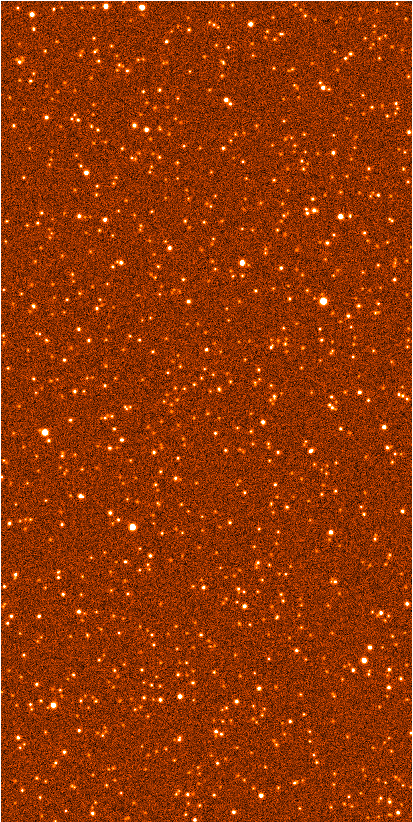
\includegraphics[width=5cm]{figures/synthetic_stars_gal_bkgd_1.png} 
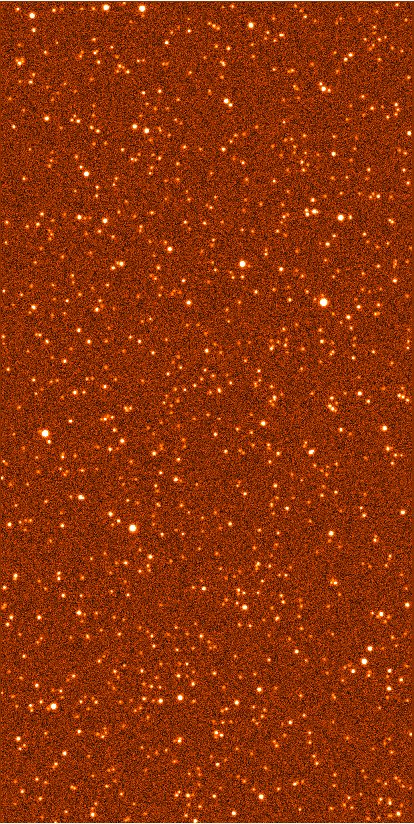
\includegraphics[width=5cm]{figures/hdrldemo_resample_DRIZZLE_single_3.png} 
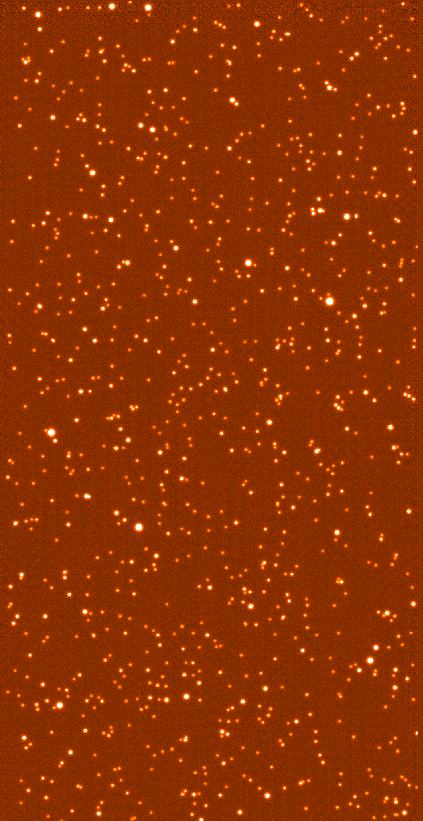
\includegraphics[width=5.115cm]{figures/hdrldemo_resample_DRIZZLE_coadd_3.png} 
\caption[]
	{\footnotesize  {\bf Left Panel:}  An input synthetic image with 1000 stellar sources.\\
	{\bf Centre Panel:}  The resampled single synthetic frame using \hdrlresample\ with {\tt --method=DRIZZLE} and {\tt --method.loop-distance=3}.\\
	{\bf Right Panel:}  The resampled tile of 10 synthetic frame using \hdrlresample\ with {\tt --method=DRIZZLE} and {\tt --method.loop-distance=3}.
	}
	\label{fig:synthetic_image}
\end{figure}


The comparison of the data products is done using a python script ({\tt compare\_image\_sex.py}).  This script runs SExtractor (\cite{bertin})
on both images with a {\tt -DETECT\_THRESH} and {\tt -ANALYSIS\_THRESH} of 5.0\,$\sigma$ and a {\tt -DETECT\_MINAREA} of 10 pixels.
A spherical, nearest-neighbour match within 1 arcsec is then done between the sources of the two resultant SExtractor catalogues.
This allows us to compare the attributes (position ($\alpha, \delta$), magnitude, FWHM, and ellipticity) of the ensemble of extracted sources
from the input synthetic images to the same sources once they have been resampled by each of the six interpolation methods.

In all five methods of image resampling, the astrometric quality of the sources is retained following interpolation.  An example of this is shown in 
Figure \ref{fig:radec_synthetic}.  Here, the absolute positions of the sources in the 10 synthetic images are compared to the absolute positions
of the sources in the image resample using the lanczos method.   Here, the median $\Delta\alpha*\cos(\delta)=0.007\pm0.03\ arcsec$ and 
$\Delta\delta=-0.001\pm0.04\ arcsec$ with the cloud of offsets spread symmetrically about the origin.  
Considering that the synthetic image pixel size is 0.20 pixels/arcsec, the astrometric accuracy is retained to better than a $\frac{1}{5}$ of one pixel (0.04 pixels).

\begin{figure}[H]
\centering
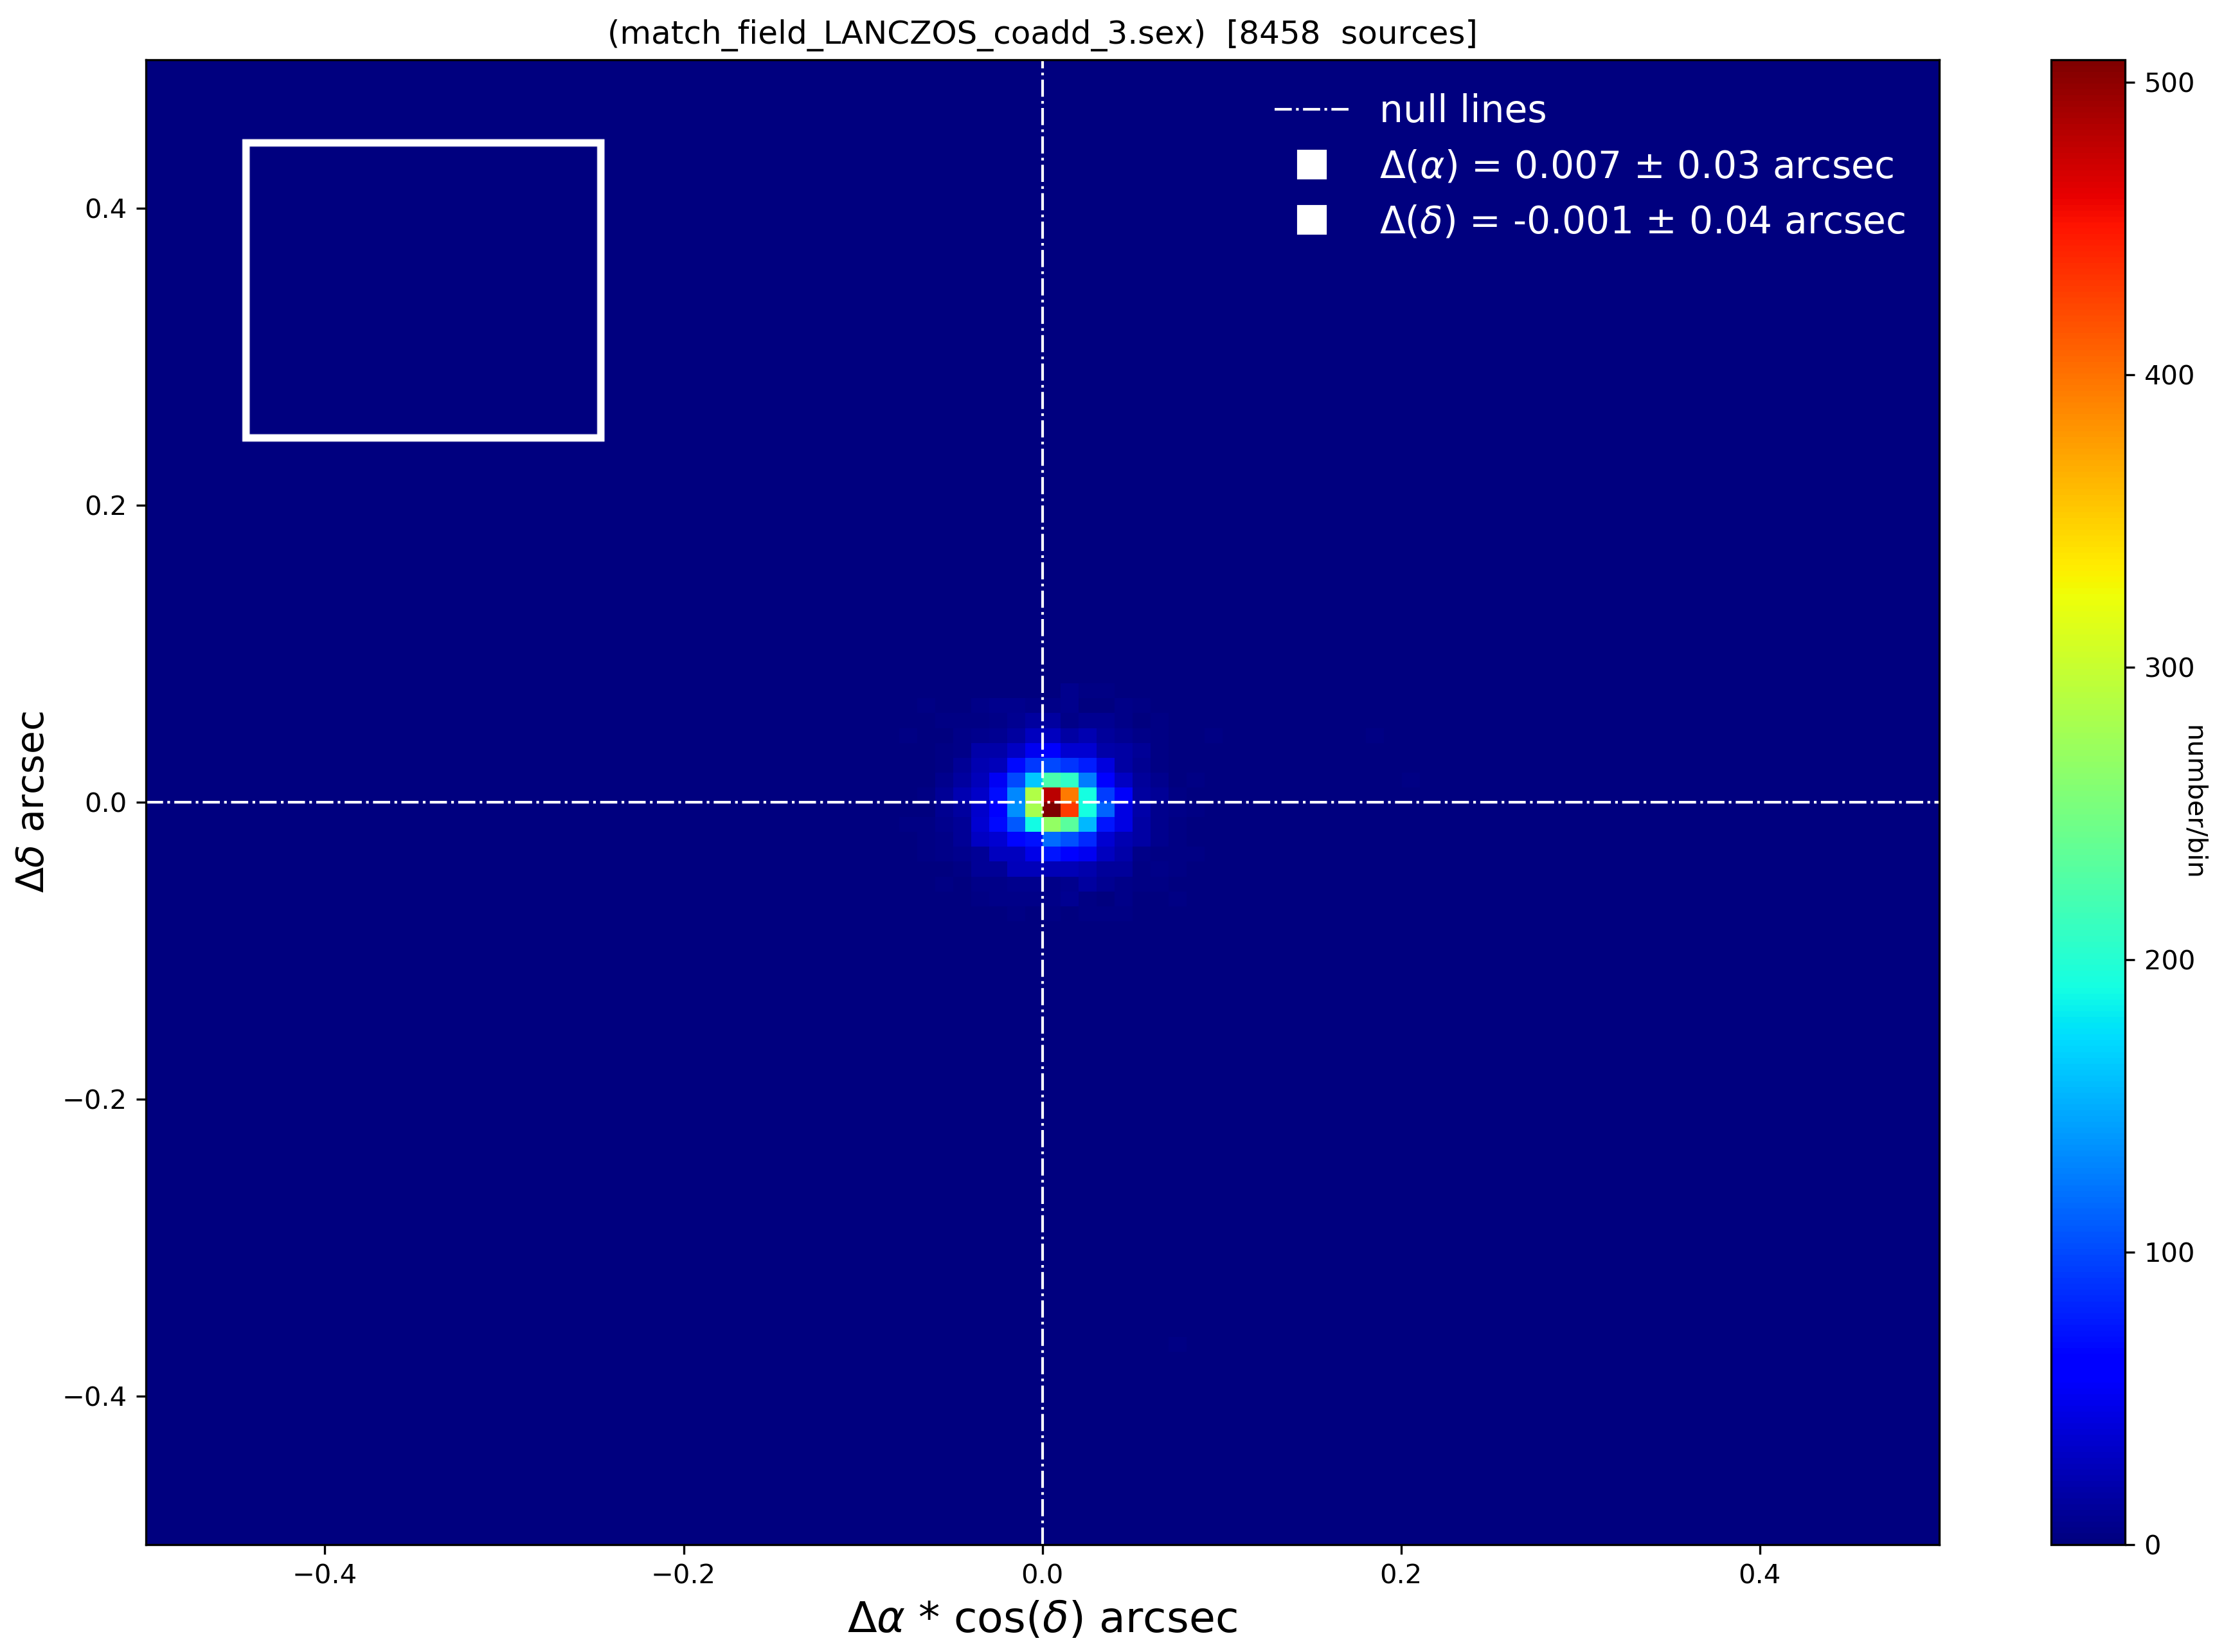
\includegraphics[width=11cm]{figures/match_field_LANCZOS_coadd_3_RA_DEC_scatter_plot.png}
\caption[]
	{\footnotesize  the astrometric quality of the \hdrlresample\ routines as measured by comparing the more than 8,000 sources in the synthetic input images,
	with those in the resampled ({\tt LANCZOS}) image tile.
	The standard deviation of the $\Delta\alpha*\cos(\delta)$ and $\Delta\delta$ distributions is 0.04 arcsec. This is significantly less than one
	pixel (0.20 pixels/arcsec).  The pixel size is indicated by the white square in the top left corner.
	}
	\label{fig:radec_synthetic}
\end{figure}

Similarly, the photometric quality is also retained following interpolation.   Figure \ref{fig:mag_synthetic} is typical of the synthetic interpolated frames, with a source magnitude match 
between the individual images and the resampled (lanczos) image tile of $\Delta(mag)=0.006\pm0.05$ magnitudes.

\begin{figure}[H]
\centering
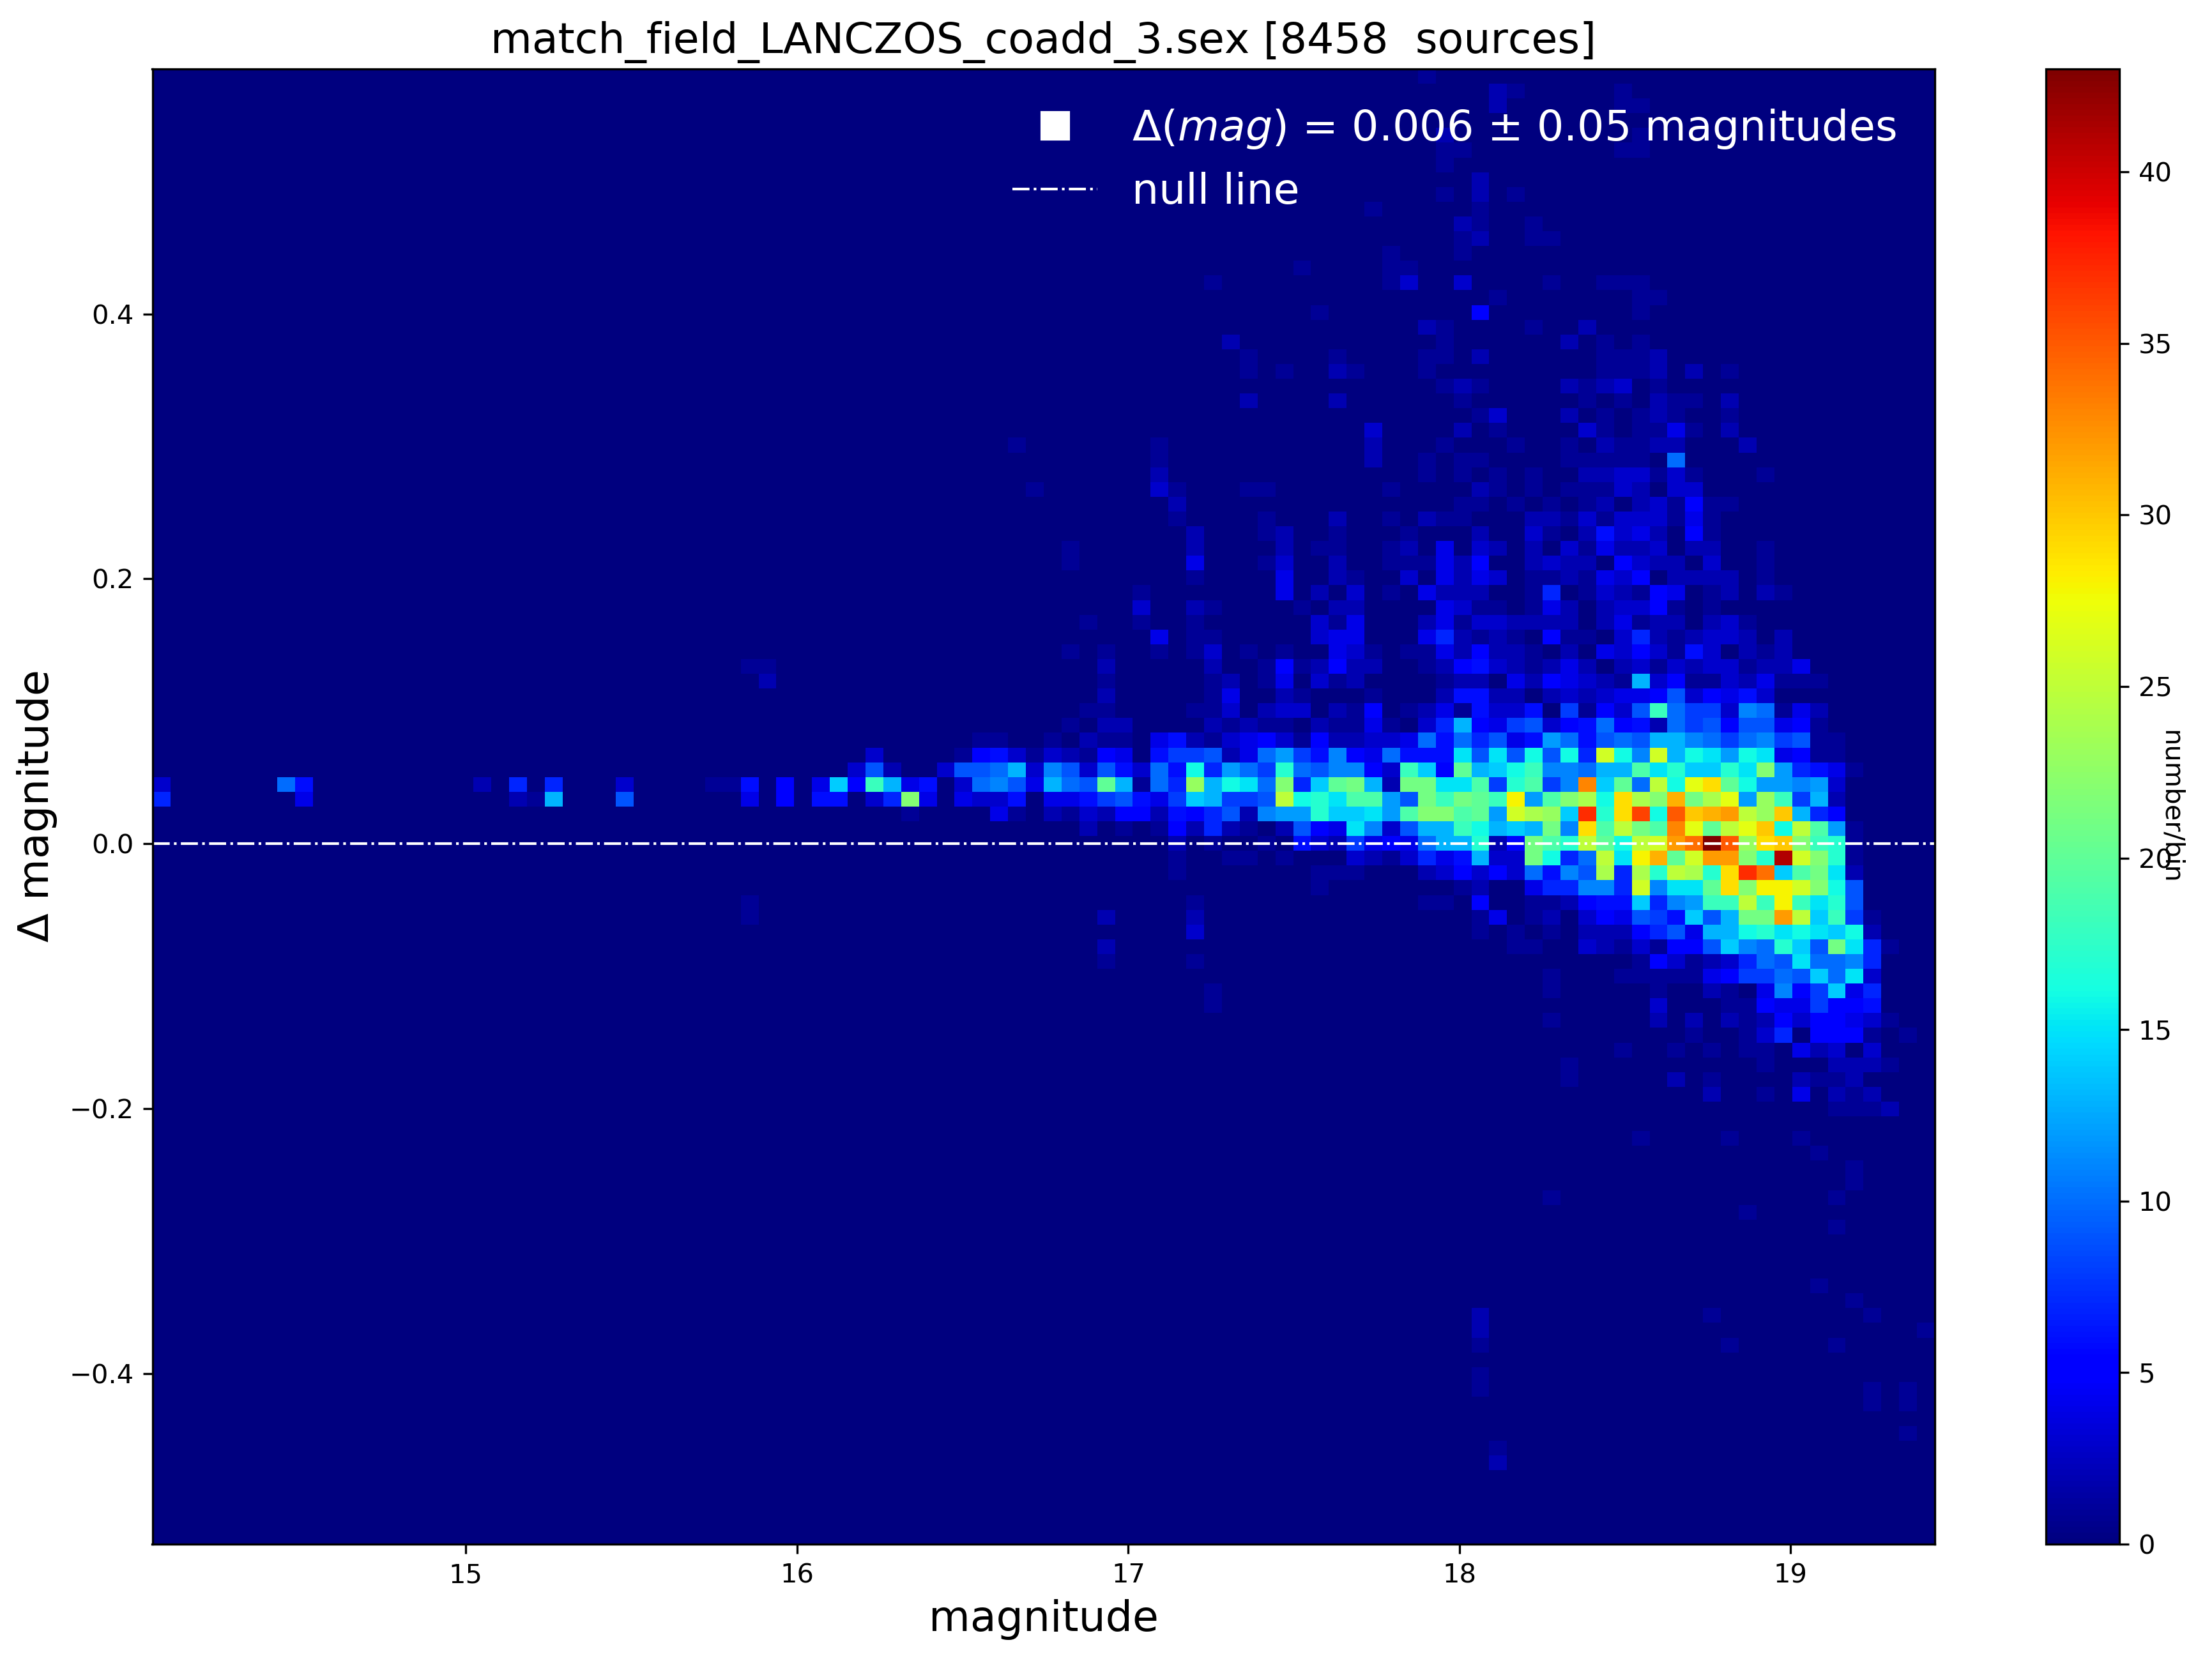
\includegraphics[width=11cm]{figures/match_field_LANCZOS_coadd_3_mag_scatter_plot.png}
\caption[]
	{\footnotesize  the photometric quality of the \hdrlresample\ routines as measured by comparing the more than 8,000 sources in the original input synthetic images
	with those in the resampled (lanczos) image tile.
	The standard deviation of the $\Delta(mag)$  distribution is 0.05 magnitudes. 	
	}
	\label{fig:mag_synthetic}
\end{figure}

As can be seen in figure \ref{fig:fwhm_ellip_synthetic}, the resampling (in this case using {\tt --method=LINEAR}) causes a slight increase in the FWHM of the sources.
This is expected for any interpolation method.   As can be seen in the left panel of Figure \ref{fig:fwhm_ellip_synthetic}, the resampling tightens the distribution of FWHM and
slightly increases it.   This is true for all resampling methods tested.   


\begin{figure}[H]
\centering
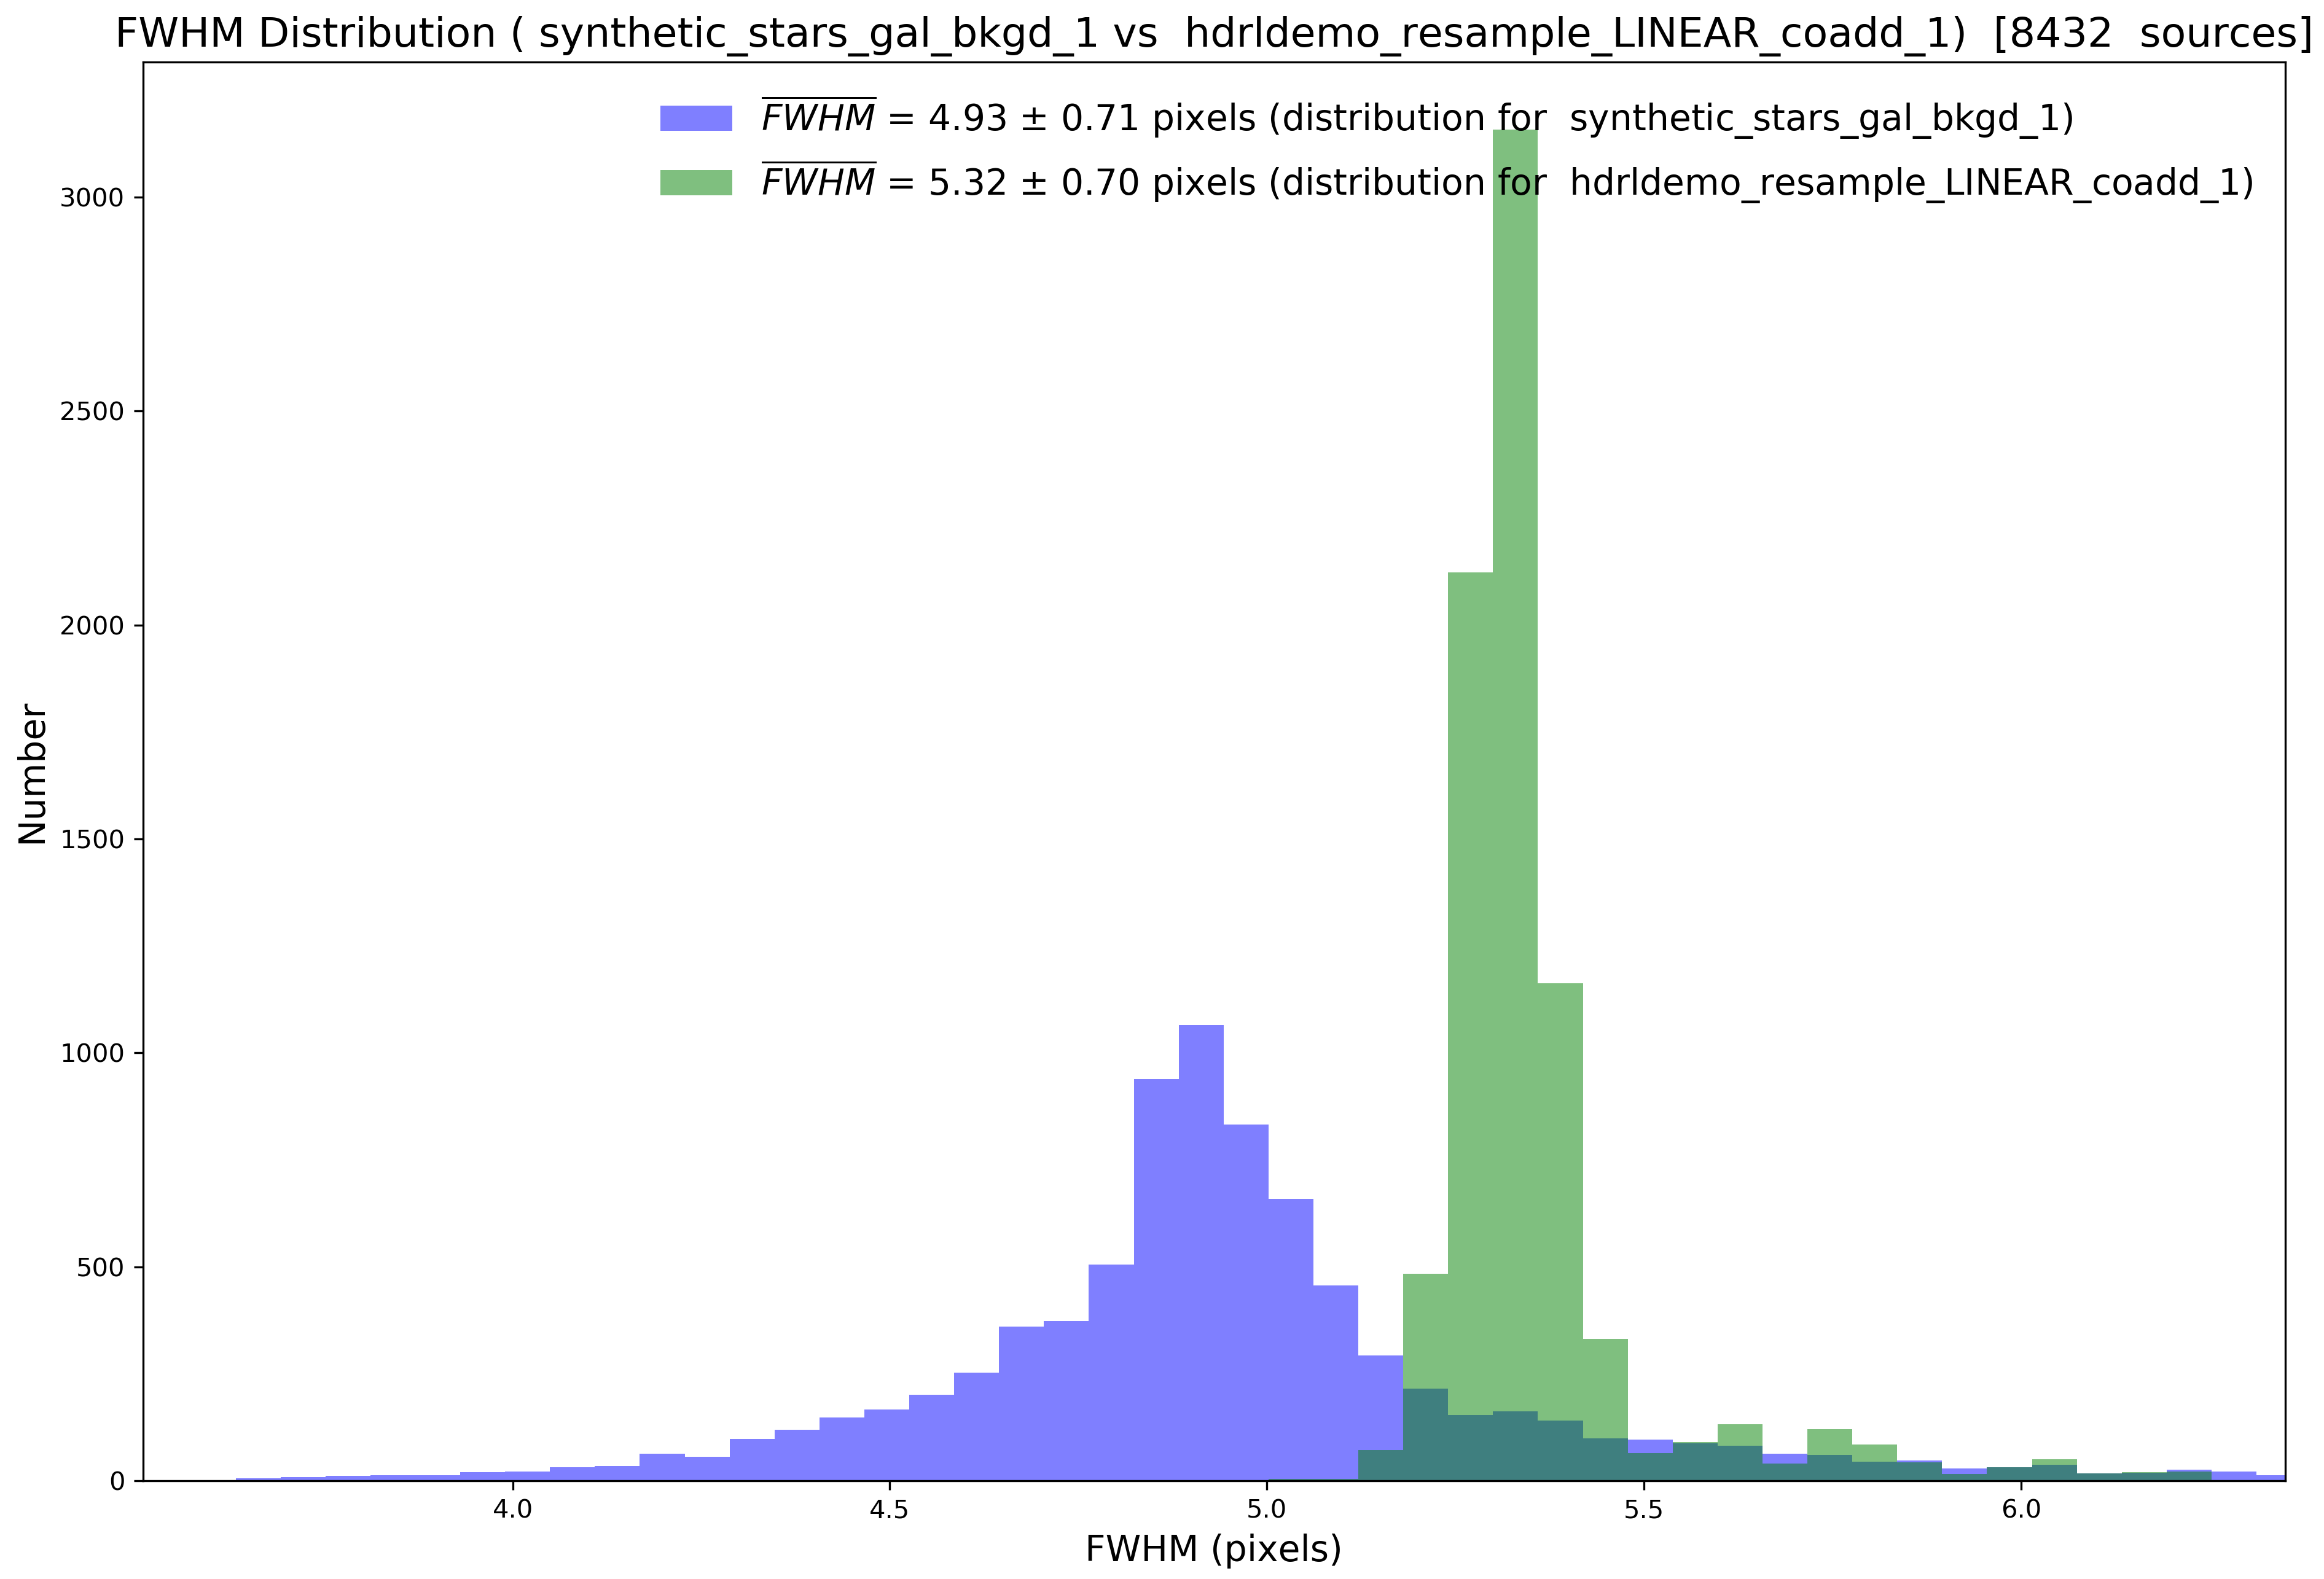
\includegraphics[width=8.4cm]{figures/match_field_LINEAR_coadd_1_FWHM_histogram.png}
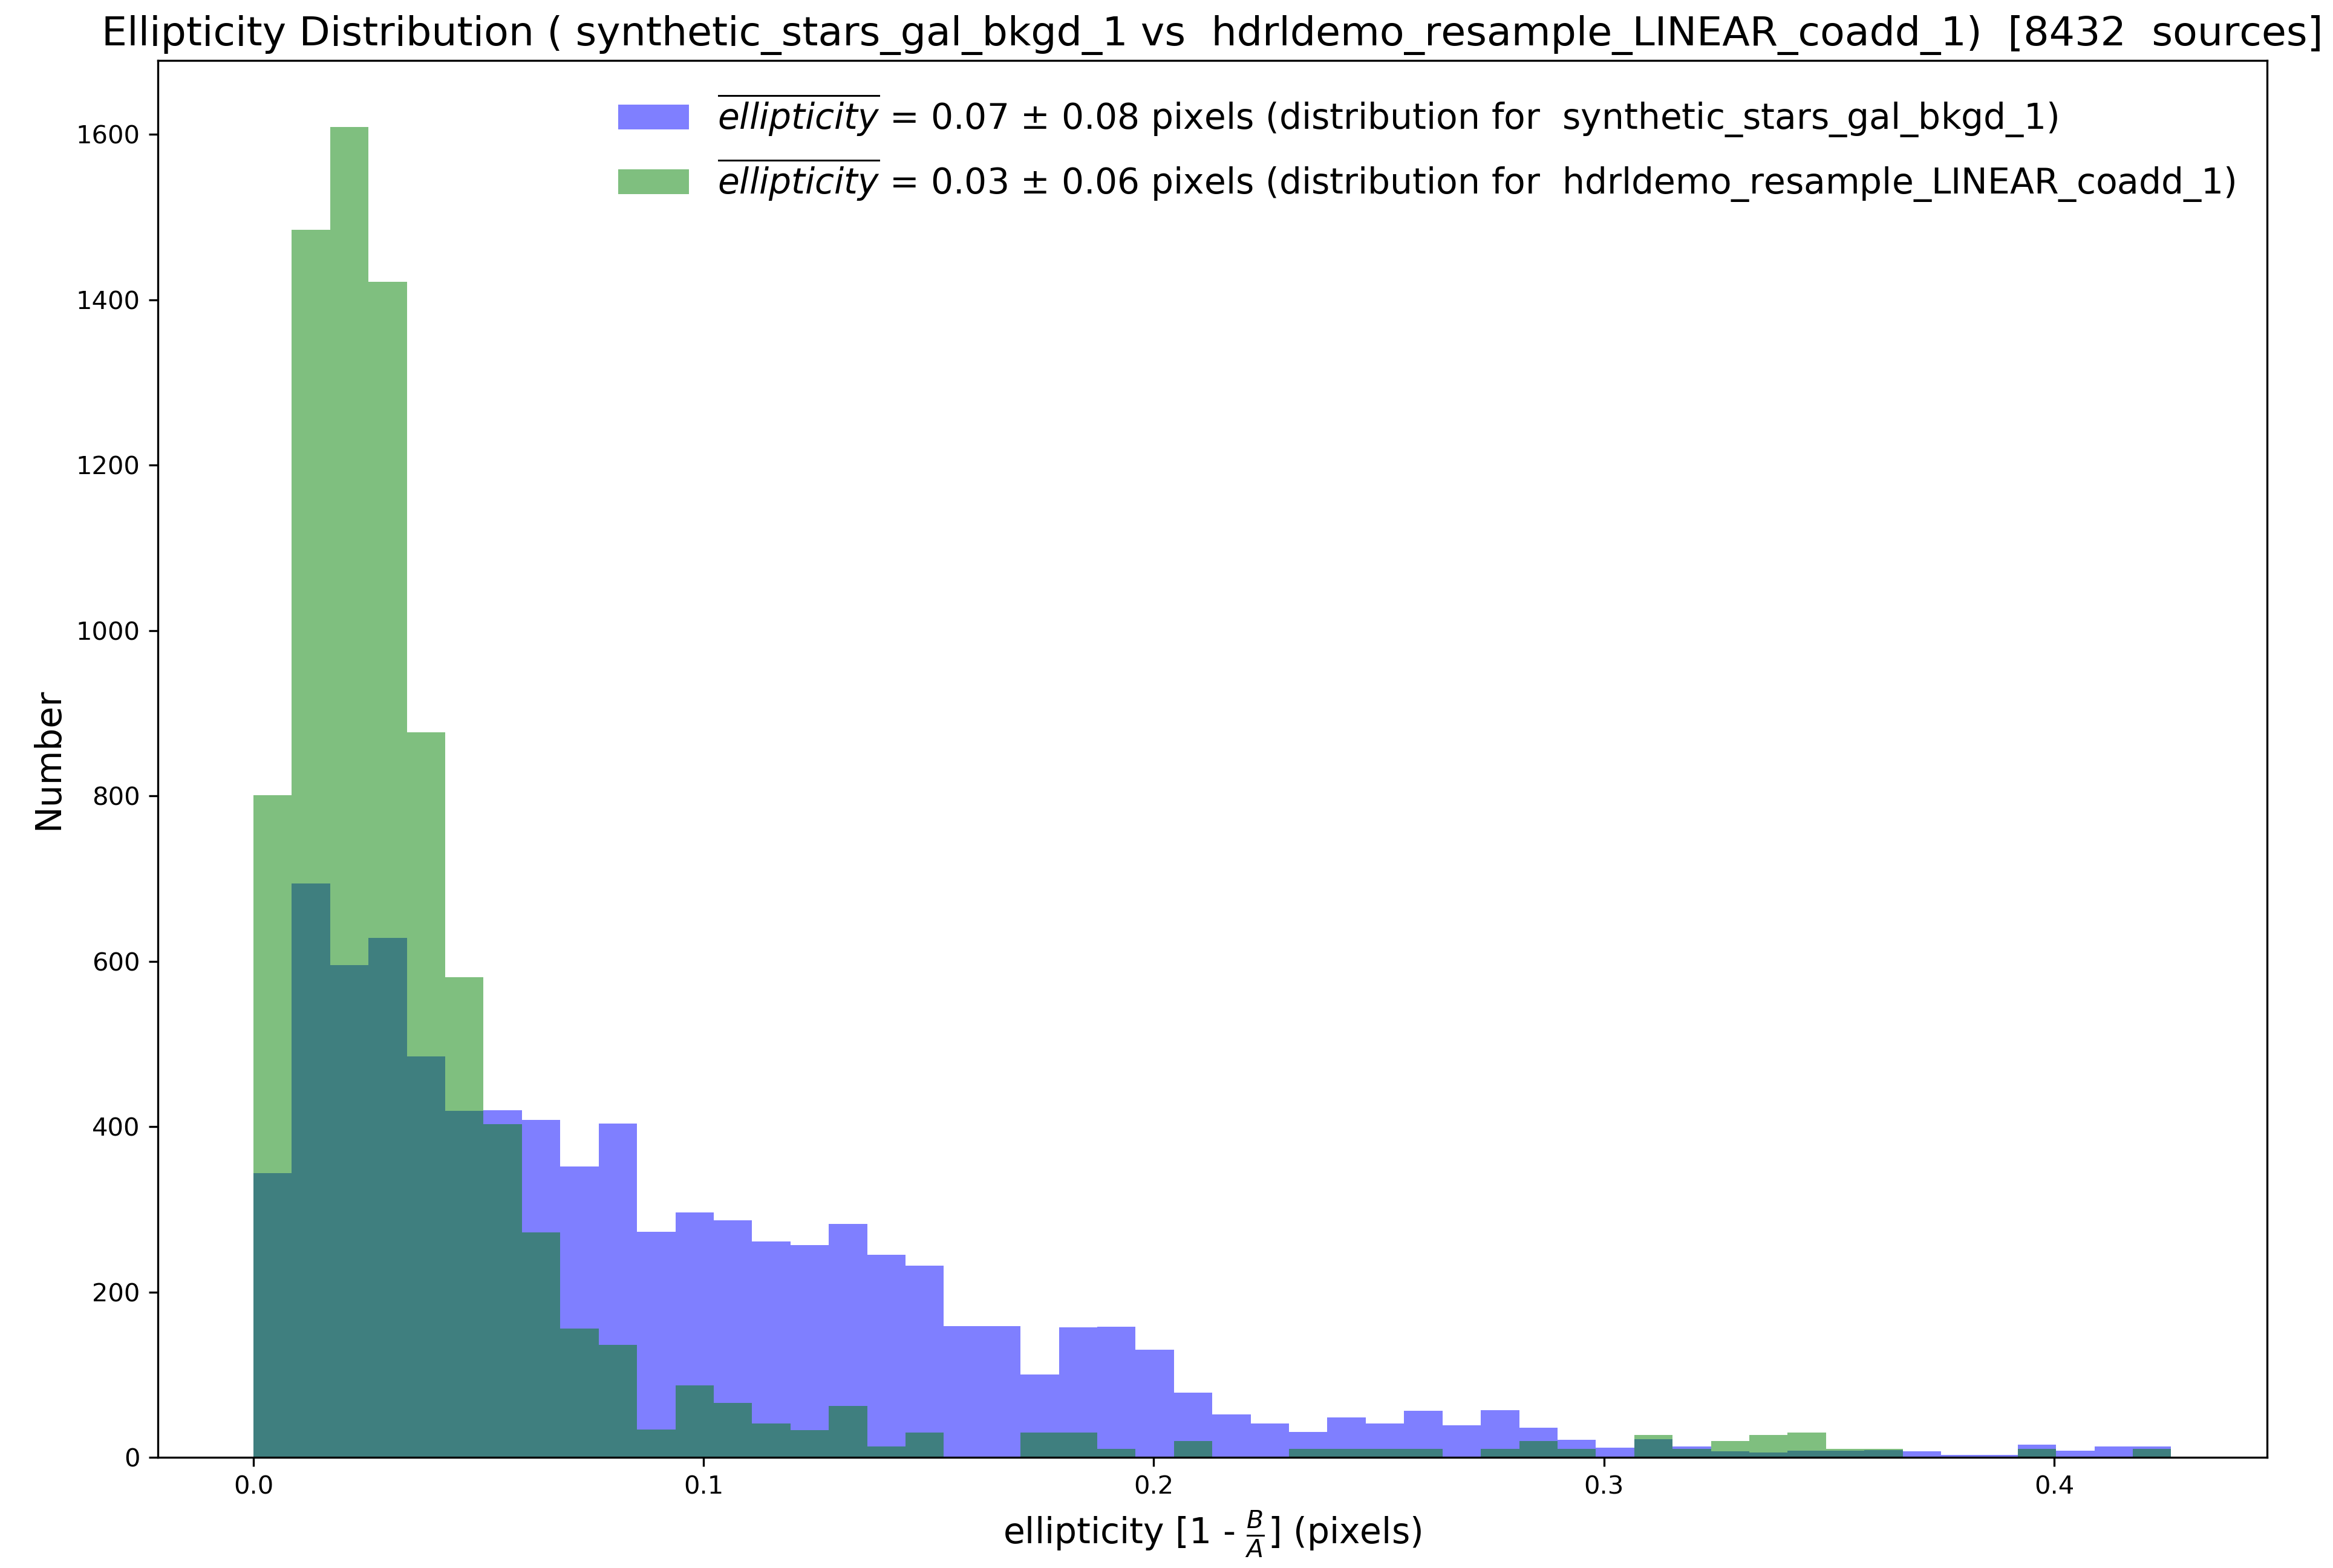
\includegraphics[width=8.4cm]{figures/match_field_LINEAR_coadd_1_ellipticity_histogram.png} 
\caption[]
	{\footnotesize  A comparison of FWHM and ellipticity for the sources in the synthetic input images (blue histograms) and those
	after resampling (green histograms).  The resampling was done with {\tt --method=LINEAR} and {\tt --method.loop-distance=1}.\\
	{\bf left panel:}    The FWHM distribution of the 8,000 sources in the synthetic field. As expected, the median FWHM, after resampling, increases slightly.  
	                          The increase in FWHM is less than 8\%.\\
	{\bf right panel:} The distribution of ellipticities.   Here, the resampling has circularised the sources.   This, too, is as expected. 
	}
	\label{fig:fwhm_ellip_synthetic}
\end{figure}




A summary of the source attributes between the input frames and the resampled images is given in Table \ref{tab:compare_synthetic}, in which the source
attributes of all six resampling methods are compared for both a single synthetic image input and a resampling of 10 synthetic images.

The largest change in the average position of the sources is $\Delta\alpha$=0.1 arcsec and $\Delta\delta$=-0.008 arcsec for the resampling {\tt method=NEAREST}.
Since this is still only one half of a pixel, this is still acceptable.  The largest change in the average magnitude  can be found in the {\tt LINEAR} resampling and
corresponds to a small shift of $\Delta$mag. = 0.06 magnitudes.
The largest change in FWHM is seen for {\tt method=LINEAR}, in which the FWHM of the synthetic
stars increase by 1.8 pixels (37\%).    A measure of the source ellipticities shows a congruent feature.   In all resampling methods the ellipticities are decreased and the distribution is
tightened, as the interpolation has the general effect of circularising the source images.  



\begin{sidewaystable}

\caption{A Summary of Comparisons Between Input Synthetic Data Images and Resultant Interpolation Images}
\footnotesize
\begin{center}
\begin{tabular}{|l|l|c|c|c|c|c|c|c|c|c|c|}                      
\toprule
synthetic\_image         				     & Interpolation	 & N$_{frames}^2$   & Nmatch & $\Delta\alpha$  & $\Delta\delta$ &  $\Delta(mag)$ & $\sigma\Delta(mag)$ & FWHM1$^3$  & FWHM2$^4$  & ellip1$^3$  & ellip2$^4$  \\
                                     & method (LD)$^1$ &                         &               & (arcsec)            & (arcsec)          &                          &                                   & (pixels)    & (pixels)   &            & \\
\midrule
synthetic\_stars\_gal\_bkgd\_single                 & DRIZZLE (1)        & single   	& 893 	& 0.000       & -0.007  	& -0.005 & 0.014          & 4.92  & 4.92  		& 0.07  & 0.07  \\
synthetic\_stars\_gal\_bkgd\_single 	   	       & DRIZZLE (3)        & single  	& 893 	& 0.000       & -0.007  	& -0.005 & 0.014 	   & 4.92  & 4.92  		& 0.07  & 0.07  \\
synthetic\_stars\_gal\_bkgd\_single 	               & LANCZOS (1)      & single  	& 892 	& 0.000       & -0.003  	& -0.005 & 0.016          & 4.92  & 4.92  		& 0.07  & 0.07    \\
synthetic\_stars\_gal\_bkgd\_single 	   	      & LANCZOS (3)      & single  	& 892 	& 0.000       & -0.004  	& -0.005 & 0.015          & 4.92  & 4.92 		& 0.07  & 0.07    \\
synthetic\_stars\_gal\_bkgd\_single 	              & LINEAR (1)          & single    	& 895 	& 0.000       & -0.007  	&  0.003 & 0.026          & 4.92  & 5.03  		& 0.07  & 0.07    \\
synthetic\_stars\_gal\_bkgd\_single 	              & LINEAR (3)          & single    	& 892 	& 0.000       & -0.006  	&  0.020 & 0.041          & 4.92  & 5.64  		& 0.07  & 0.06    \\
synthetic\_stars\_gal\_bkgd\_single 	              & NEAREST (1)      & single   	& 893 	& 0.000       & -0.007  	& -0.005 & 0.014          & 4.92  & 4.92  		& 0.07  & 0.07    \\
synthetic\_stars\_gal\_bkgd\_single 	              & NEAREST (3)      & single   	& 893 	& 0.000       & -0.007  	& -0.005 & 0.014          & 4.92  & 4.92  		& 0.07  & 0.07    \\
synthetic\_stars\_gal\_bkgd\_single 	              & QUADRATIC (1)  & single 	& 890 	& 0.000       & -0.007  	& -0.004 & 0.015          & 4.92  & 4.92  		& 0.07  & 0.07    \\
synthetic\_stars\_gal\_bkgd\_single 	              & QUADRATIC (3)  & single 	& 889 	& 0.000       & -0.007  	& -0.004 & 0.015          & 4.92  & 4.93   		& 0.07  & 0.07    \\
synthetic\_stars\_gal\_bkgd\_single 	              & RENKA (1)           & single 	& 892 	& 0.000       & -0.007  	& -0.005 & 0.015          & 4.92  & 4.92 		& 0.07  & 0.07   \\
synthetic\_stars\_gal\_bkgd\_single                & RENKA (3)           & single  	& 892 	& 0.000       & -0.007  	& -0.004 & 0.014          & 4.92  & 4.92  		& 0.07  & 0.07    \\
\midrule
synthetic\_stars\_gal\_bkgd\_1$\to$10   	& DRIZZLE (1)        &10    		&  8,587 	& 0.001       & -0.008  	& 0.024  & 0.06 	& 4.93  & 5.01  			& 0.07    & 0.03  \\
synthetic\_stars\_gal\_bkgd\_1$\to$10   	& DRIZZLE (3)        &10    		&  8,587 	& 0.001       & -0.008  	& 0.024  & 0.06 	& 4.93  & 5.01 			& 0.07    & 0.03  \\
synthetic\_stars\_gal\_bkgd\_1$\to$10   	& LANCZOS (1)      &10    		&  8,619 	& -0.017      & 0.003   	& 0.024  & 0.06		& 4.93  & 4.97  			& 0.07    & 0.03  \\
synthetic\_stars\_gal\_bkgd\_1$\to$10   	& LANCZOS (3)     &10    			&  8,629 	& 0.007       & -0.001  	& 0.020  & 0.06 	& 4.93  & 4.88  			& 0.07    & 0.03  \\
synthetic\_stars\_gal\_bkgd\_1$\to$10   	& LINEAR (1)         &10 	   		&  8,603 	& 0.056       & -0.006  	& 0.040  & 0.07 	& 4.93  & 5.32  			& 0.07    & 0.03  \\
synthetic\_stars\_gal\_bkgd\_1$\to$10   	& LINEAR (3)         &10 	   		&  8,508 	& 0.051       & -0.005  	& 0.064  & 0.07  	& 4.93  & 6.76   		& 0.07    & 0.03  \\
synthetic\_stars\_gal\_bkgd\_1$\to$10   	& NEAREST (1)     &10    			&  8,390 	& 0.099       & -0.008  	&-0.007  & 0.01 	& 4.93  & 4.91 			& 0.07    & 0.07  \\
synthetic\_stars\_gal\_bkgd\_1$\to$10   	& NEAREST (3)     &10    			&  8,390 	& 0.099       & -0.008  	&-0.007  & 0.01 	& 4.93  & 4.91  			& 0.07    & 0.07  \\
synthetic\_stars\_gal\_bkgd\_1$\to$10   	& QUADRATIC (1) &10  			&  8,589 	& 0.027       & -0.005  	& 0.031  & 0.07 	& 4.93  & 5.18  			& 0.07   & 0.03  \\
synthetic\_stars\_gal\_bkgd\_1$\to$10   	& QUADRATIC (3) &10  			&  8,569	& 0.018       & -0.003  	& 0.042  & 0.06 	& 4.93  & 5.74  			& 0.07   & 0.03  \\
synthetic\_stars\_gal\_bkgd\_1$\to$10   	& RENKA (1)          &10 	   		&  8,581 	& 0.006       & -0.005  	& 0.029  & 0.07 	& 4.93  & 5.07  			& 0.07   & 0.03  \\
synthetic\_stars\_gal\_bkgd\_1$\to$10   	& RENKA (3)          &10	   		&  8,581 	& 0.003       & -0.004  	& 0.029  & 0.07 	& 4.93  & 5.08  			& 0.07   & 0.03  \\
\bottomrule


\end{tabular}	
\end{center}																											

\label{tab:compare_synthetic}
\noindent{
		$^1$ The interpolation method and loop-distance used ({\tt --method.loop-distance}).\\
		$^2$ The total number of synthetic input images combined during the resampling.\\
		$^3$ FWHM1 and ellip1 refer to the synthetic input images.\\
		$^4$ FWHM2 and ellip2 refer to the resampled images.}
\end{sidewaystable}

\normalsize

\subsection{Results from HAWK-I Globular Cluster Images}
\label{sect:hawki1}


To test the \hdrlresample\ routines a series of large-field HAWK-I exposures were processed.  
This data includes the globular cluster fields mapping M30 and NGC288.
The data for M30 is from 2015-10-31 with OBS.ID=200203309, while the data for NGC288 is from 2016-11-22 with OBS.ID=200203307.
Both data sets have PROG.ID=60.A-9800(L).

All data has been processed using the HAWK-I pipeline version 2.4.6, with the intermediate pipeline science products 
({\tt BASIC\_CALIBRATED\_SCI} and {\tt BASIC\_VAR\_MAP}) acting as input for the \hdrlint\  and image combination routines.
Each data set consisted of 25, calibrated science frames (dark-corrected, gain-corrected, flat-fielded, and astrometrically and photometrically calibrated), with each being a MEF
of four detectors for a total of 100 individual exposures.
These 100 images were resampled using each of the methods available in \hdrlresample, {\tt NEAREST, LINEAR, QUADRATIC, RENKA, LANCZOS,
and DRIZZLE}, and each was executed with both a loop distance of 1 and 3 pixels ({\tt --method.loop-distance}).
The resulting image tiles are then compared to the original input images.

The comparison of the data products is done using a python script ({\tt compare\_image\_sex.py}).  This script runs SExtractor (\cite{bertin})
on both images with a {\tt -DETECT\_THRESH} and {\tt -ANALYSIS\_THRESH} of 5.0\,$\sigma$ and a {\tt -DETECT\_MINAREA} of 10 pixels.
A spherical, nearest-neighbour match within 1 arcsec is then done between the sources of the two resultant SExtractor catalogues.
This allows us to compare the attributes (position ($\alpha, \delta$), magnitude, FWHM, and ellipticity) of the ensemble of extracted sources
from the original input images to the same sources once they have been resampled by each of the six interpolation methods.


% NGC288:
\subsubsection{NGC288}

An example of the \hdrlresample\ product is shown in figure \ref{fig:hawki_ngc288}.  A comparison with the combined frames from the
HAWK-I pipeline (combined with {\tt hawki\_science\_postprocess} show qualitatively very similar results.


\begin{figure}[H]
\centering
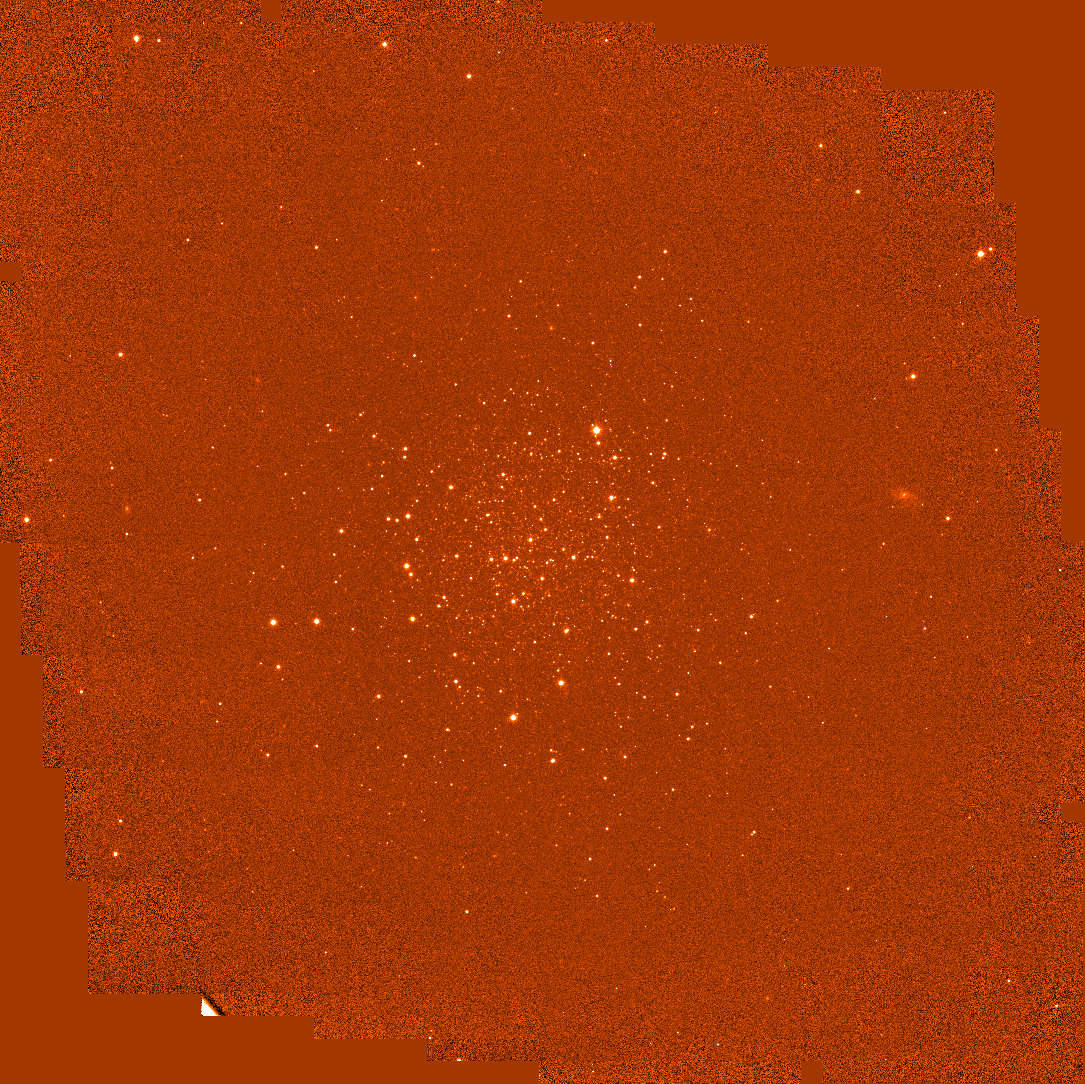
\includegraphics[width=8.4cm]{figures/Distortion_NGC288_TILED_IMAGE.png}
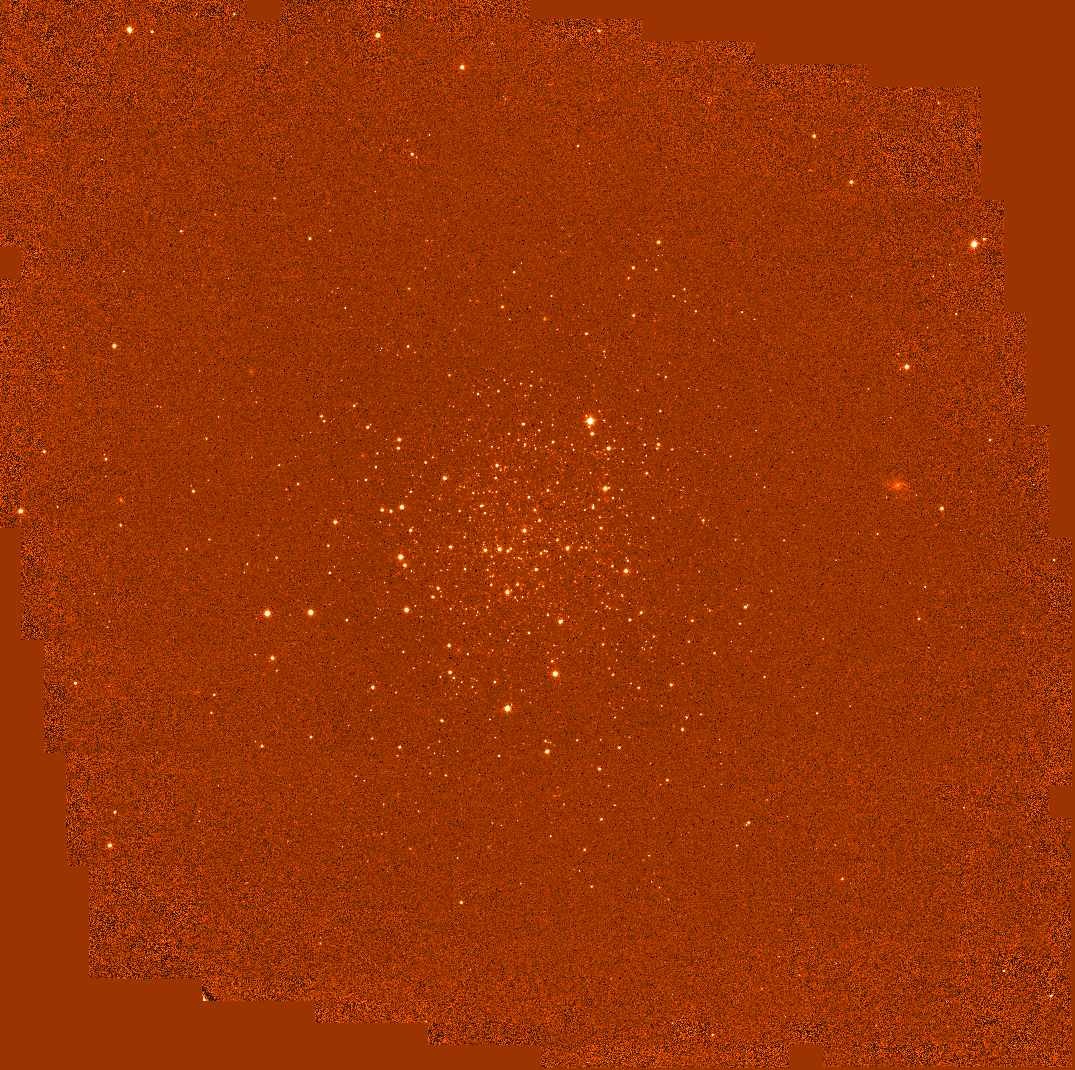
\includegraphics[width=8.4cm]{figures/hdrldemo_resample_DRIZZLE_HAWKI_NGC288_1.png} 
\caption[]
	{\footnotesize  The final tile image made from 100 HAWK-I images of the NGC\,288 field:\\
	{\bf left panel:}    as creating by the HAWK-I pipeline v. 2.4.6 routine {\tt hawki\_science\_postprocess}\\
	{\bf right panel:} as resampled and combined using \hdrlresample\ with {\tt --method=DRIZZLE} and {\tt --method.loop-distance=1}.\\
	}
	\label{fig:hawki_ngc288}
\end{figure}

In all five methods of image resampling, the astrometric quality of the sources is retained following interpolation.  An example of this is shown in 
figure \ref{fig:radec_NGC288}.  Here, the absolute positions of the sources in the 100 input HAWK-I images is compared to the absolute positions
of the sources in the image resample using the drizzle method.   Here, the median $\Delta\alpha*\cos(\delta)=0.001\pm0.07\ arcsec$ and 
$\Delta\delta=0.003\pm0.07\ arcsec$ with the cloud of offsets spread symmetrically about the origin.  
Considering that the HAWK-I pixel size is 0.106 pixels/arcsec, the astrometric accuracy is retained to better than a fraction of one pixel (0.66 pixels).

\begin{figure}[H]
\centering
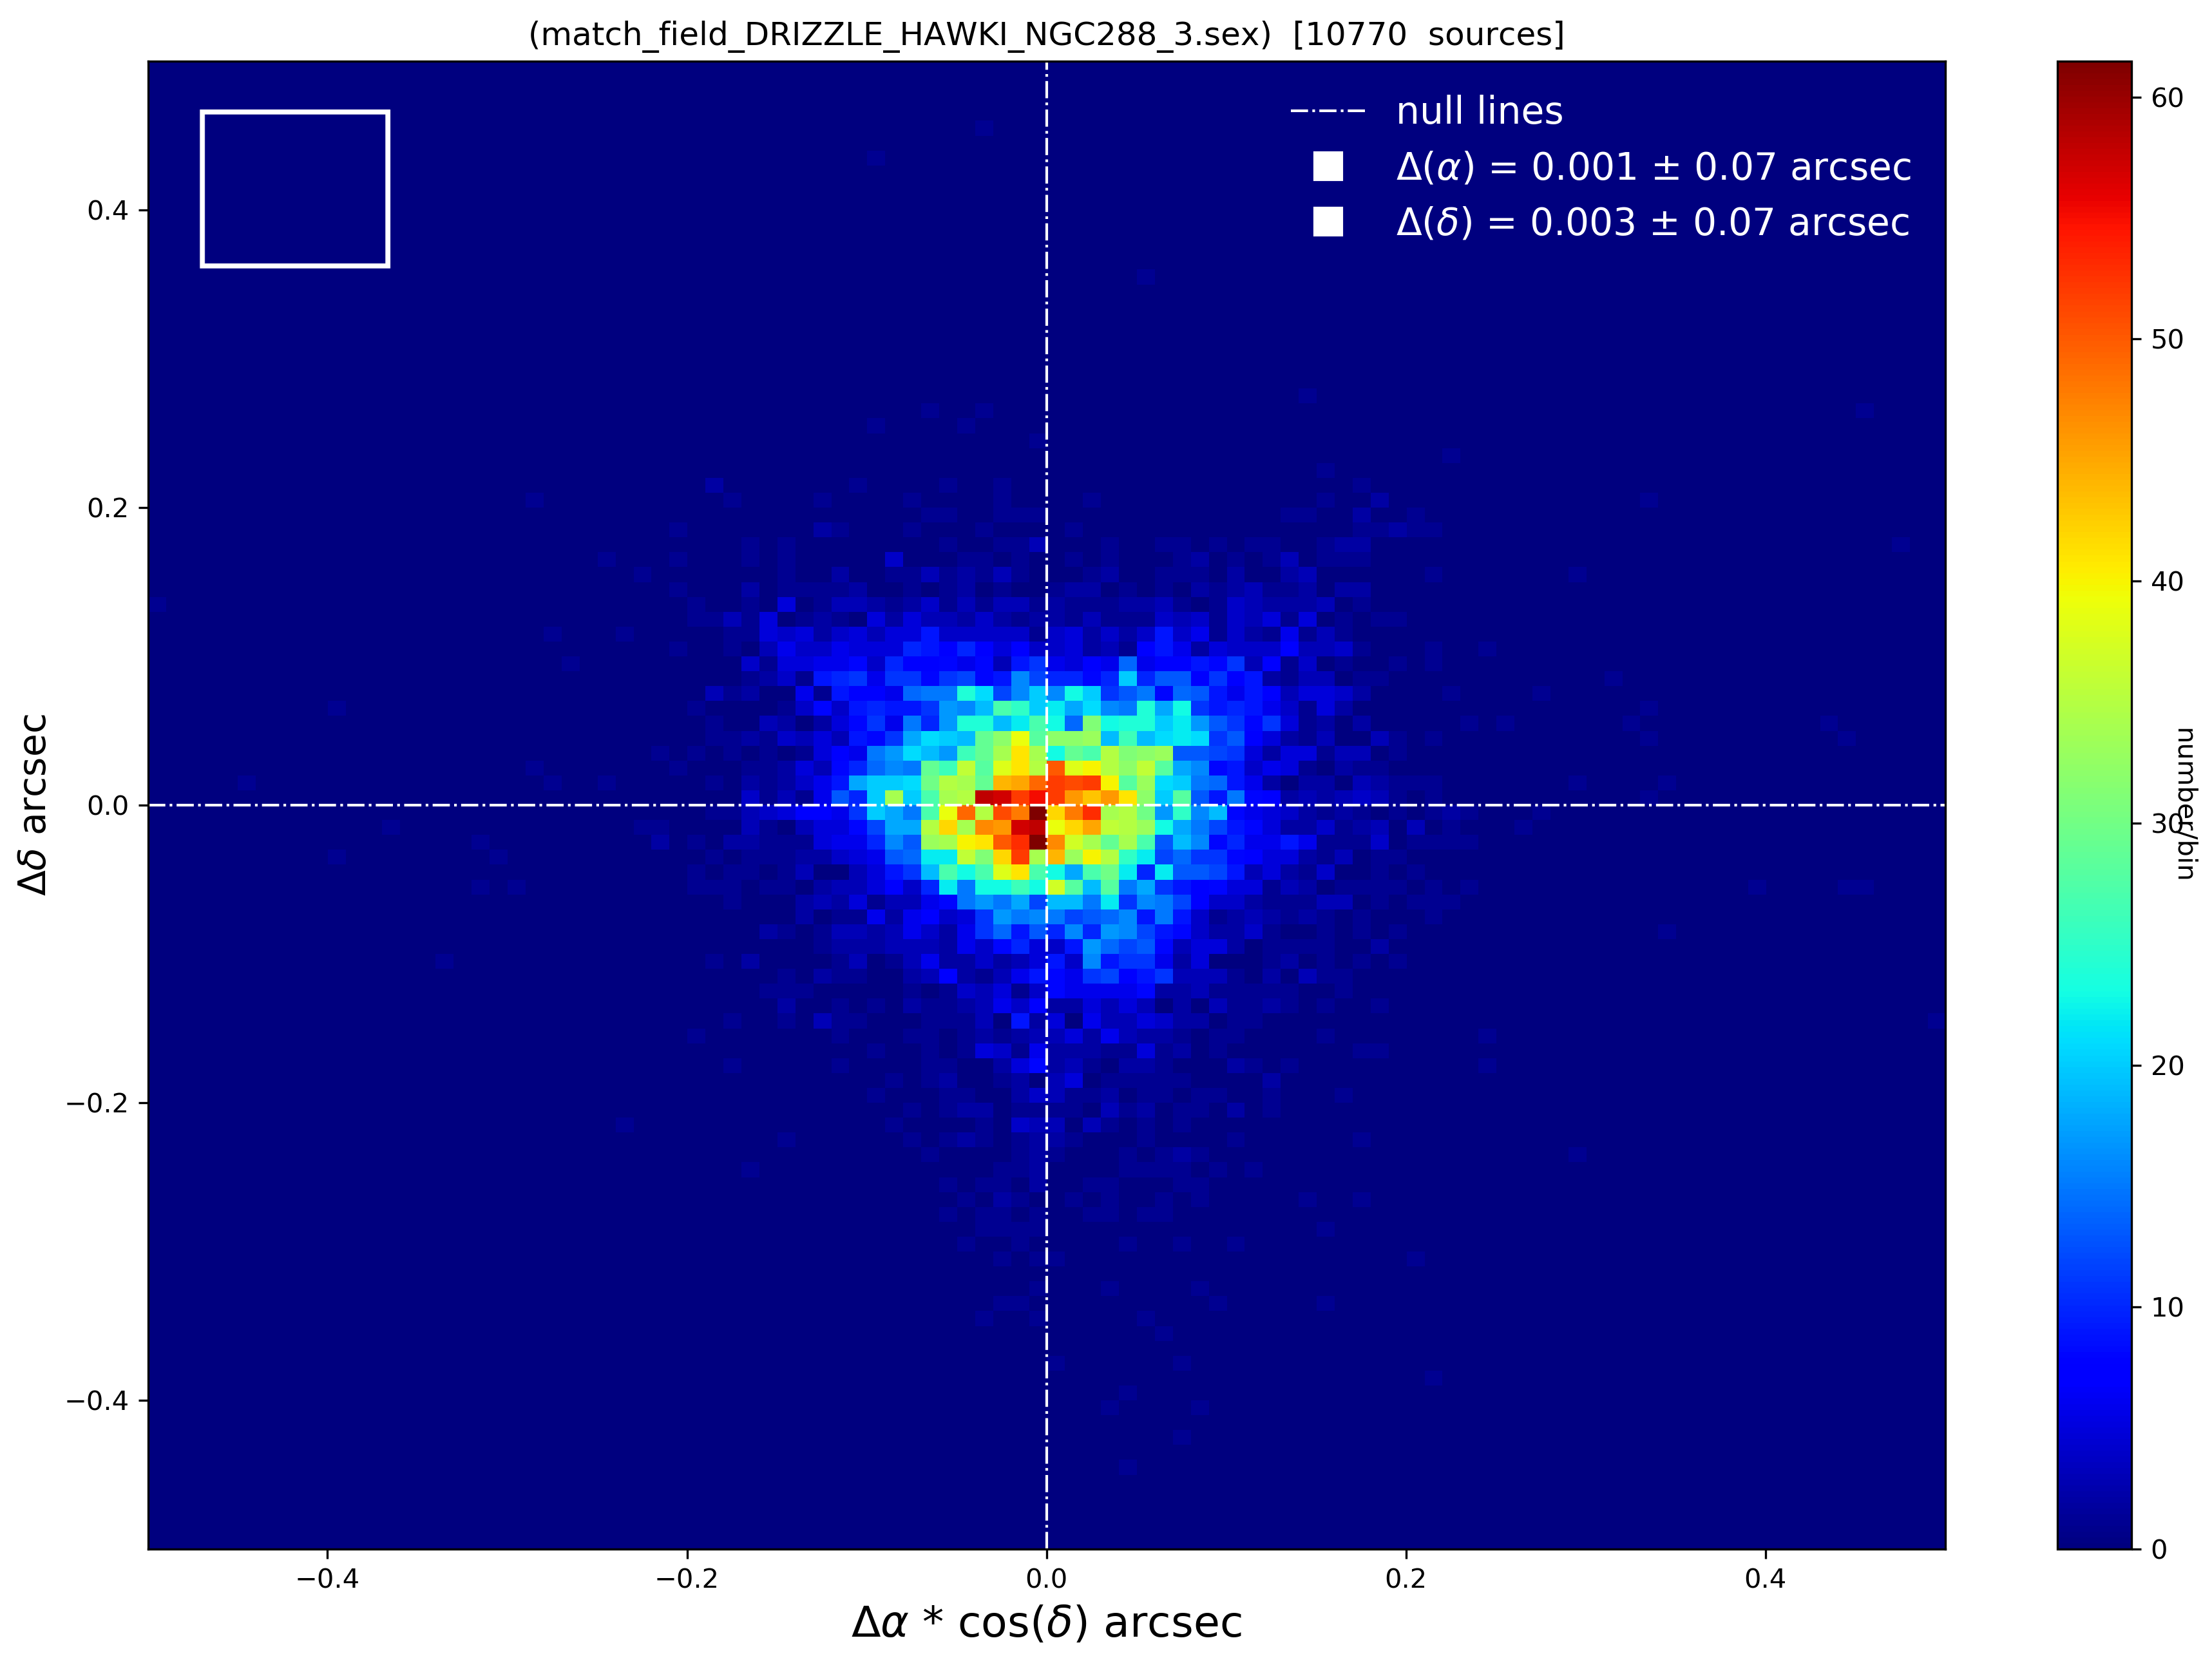
\includegraphics[width=11cm]{figures/match_field_DRIZZLE_HAWKI_NGC288_3_RA_DEC_scatter_plot.png}
\caption[]
	{\footnotesize  the astrometric quality of the \hdrlresample\ routines as measured by comparing the more than 10,000 sources in original input HAWK-I images
	with those in the resampled (drizzle) image tile of Figure \ref{fig:hawki_ngc288}.
	The standard deviation of the $\Delta\alpha*\cos(\delta)$ and $\Delta\delta$ distributions is 0.07 arcsec. This is significantly less than one HAWK-I
	pixel (0.106 pixels/arcsec).  The pixel size is indicated by the white square in the top left corner.
	}
	\label{fig:radec_NGC288}
\end{figure}


\begin{figure}[H]
\centering
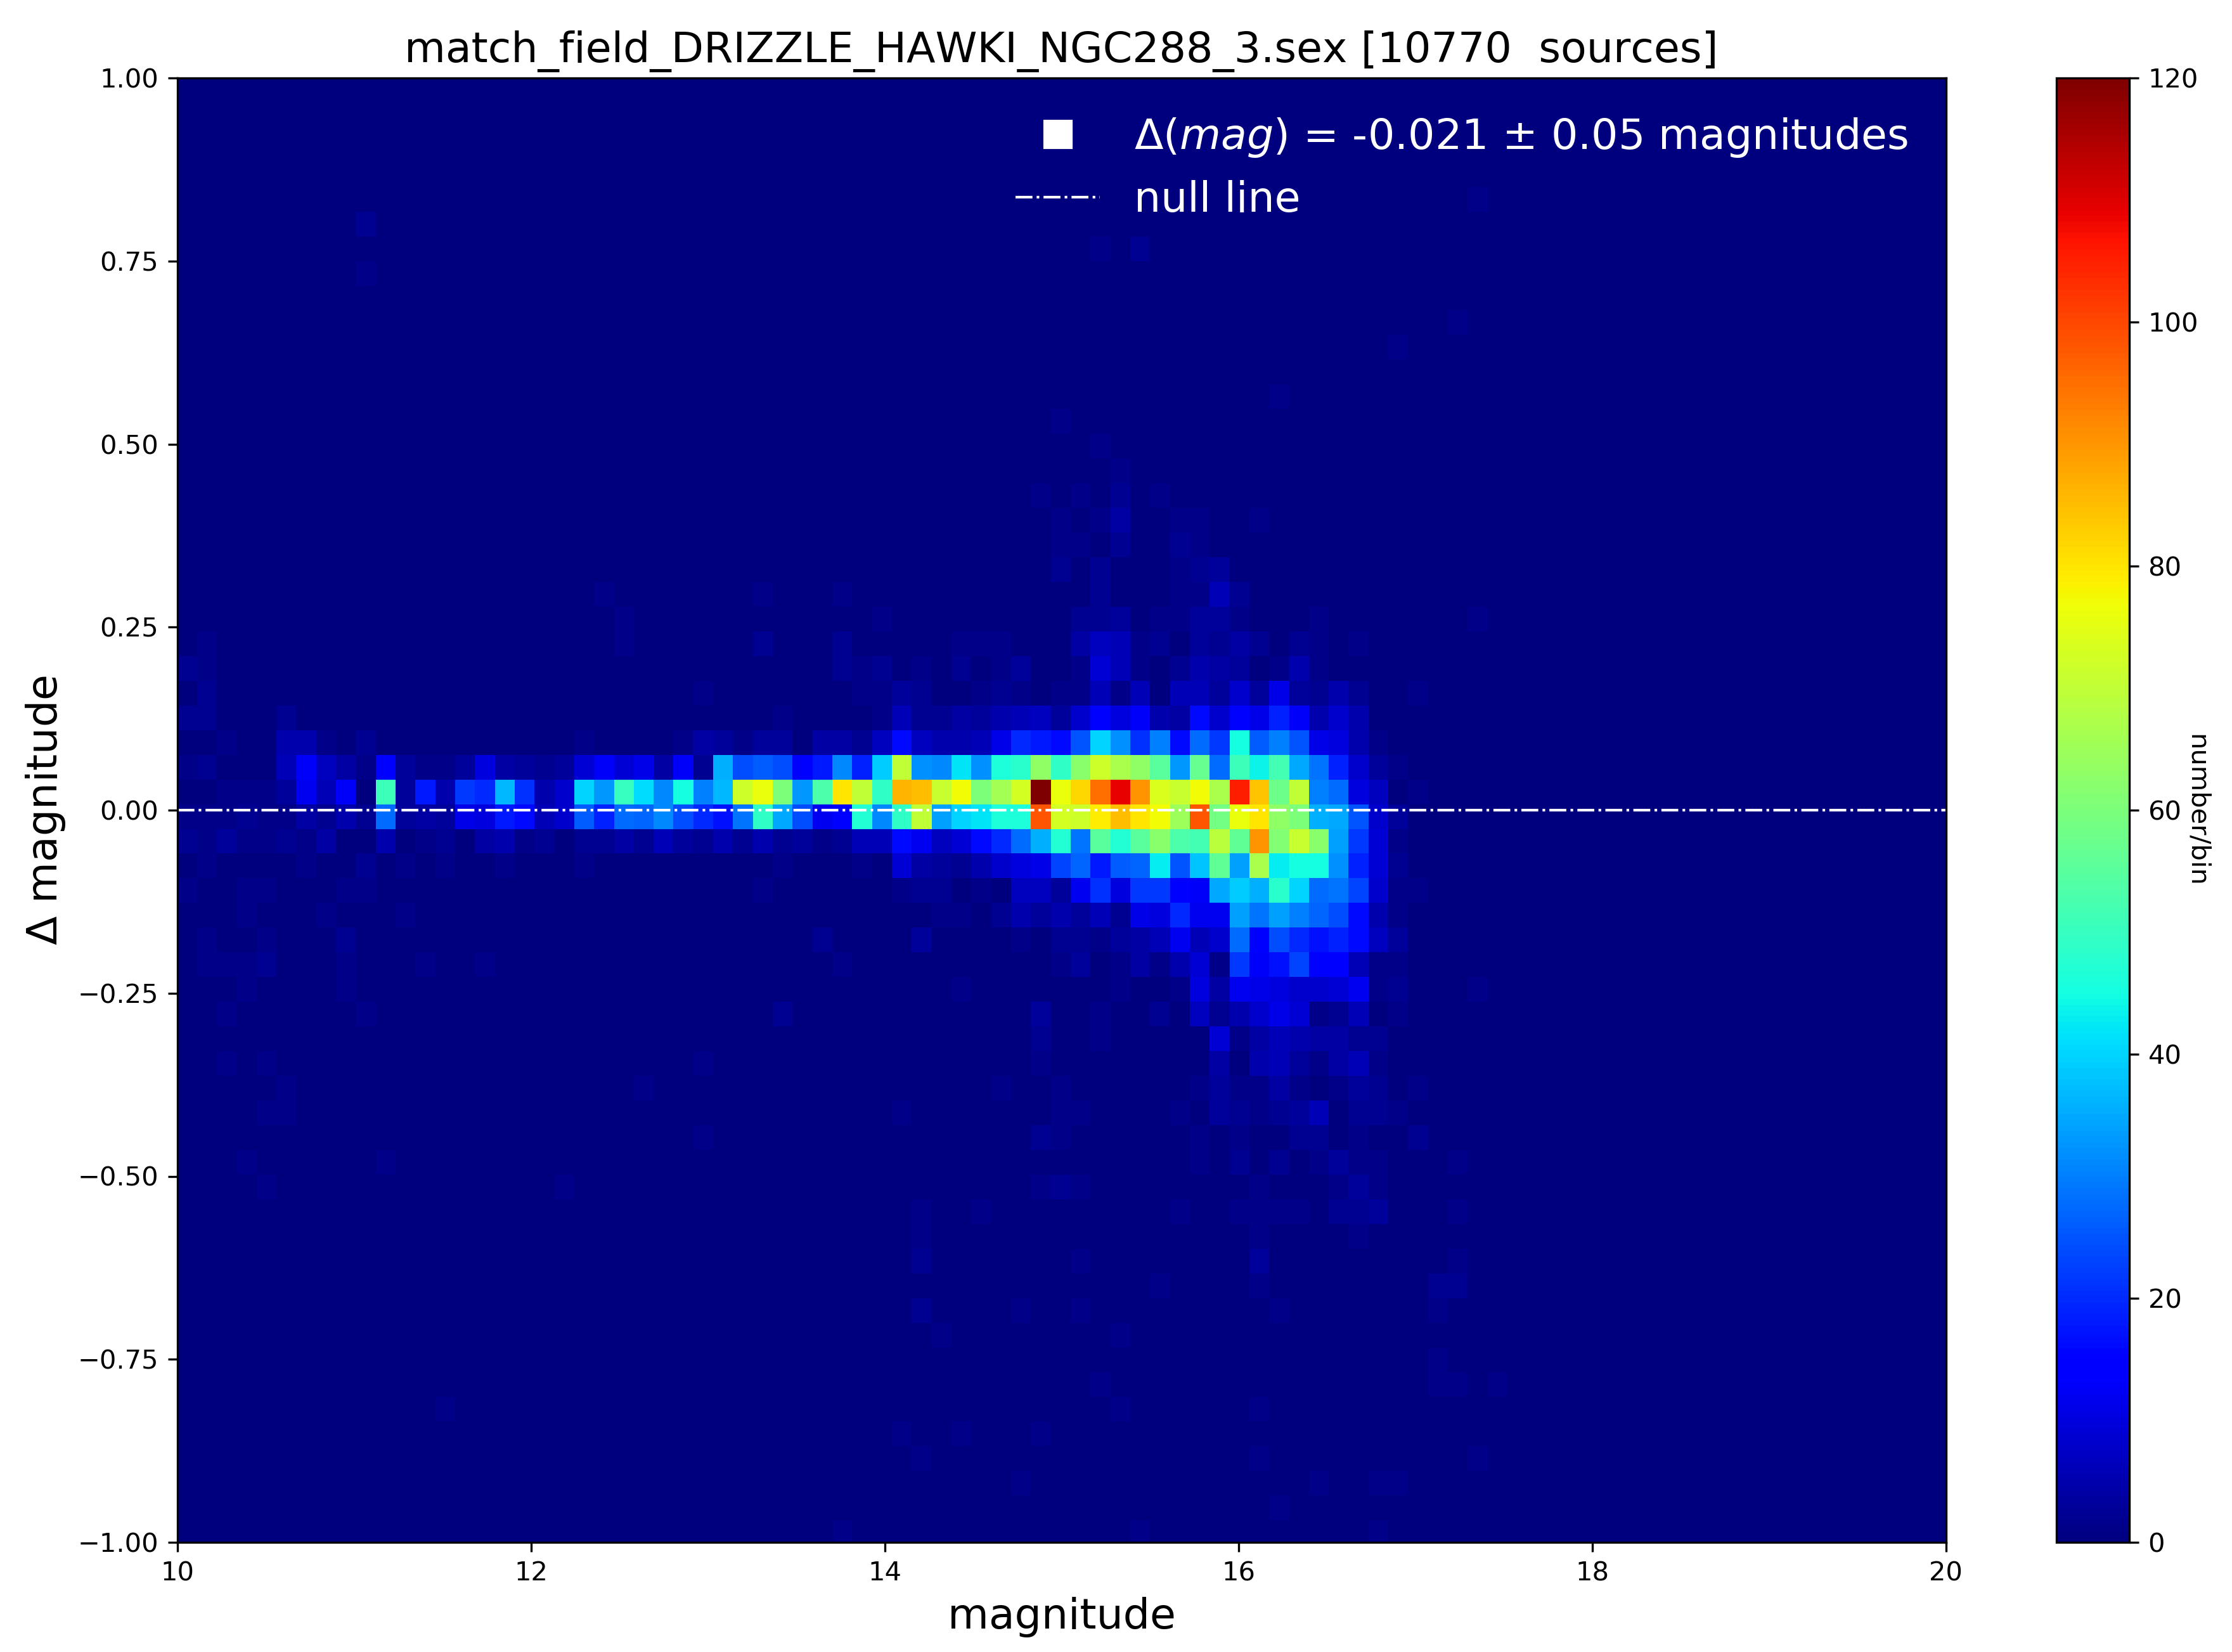
\includegraphics[width=11cm]{figures/match_field_DRIZZLE_HAWKI_NGC288_3_mag_scatter_plot.png}
\caption[]
	{\footnotesize  the photometric quality of the \hdrlresample\ routines as measured by comparing the more than 10,000 sources in original input HAWK-I images
	with those in the resampled (drizzle) image tile of Figure \ref{fig:hawki_ngc288} (right panel).
	The standard deviation of the $\Delta(mag)$  distribution is 0.05 magnitudes. 	
	}
	\label{fig:mag_NGC288}
\end{figure}

Similarly, the photometric quality is also retained following interpolation.   Figure \ref{fig:mag_NGC288} is typical of all interpolated frames, with a source magnitude match 
between the individual HAWK-I images and the resampled (drizzle) image tile of $\Delta(mag)=-0.02\pm0.05$ magnitudes.

As can be seen in figure \ref{fig:fwhm_ellip_NGC288}, the resampling causes a slight increase in the FWHM of the sources and a decrease in the source ellipticities.
This is expected, since the resampling will cause a circularisation and homogenisation of the source shapes.


\begin{figure}[H]
\centering
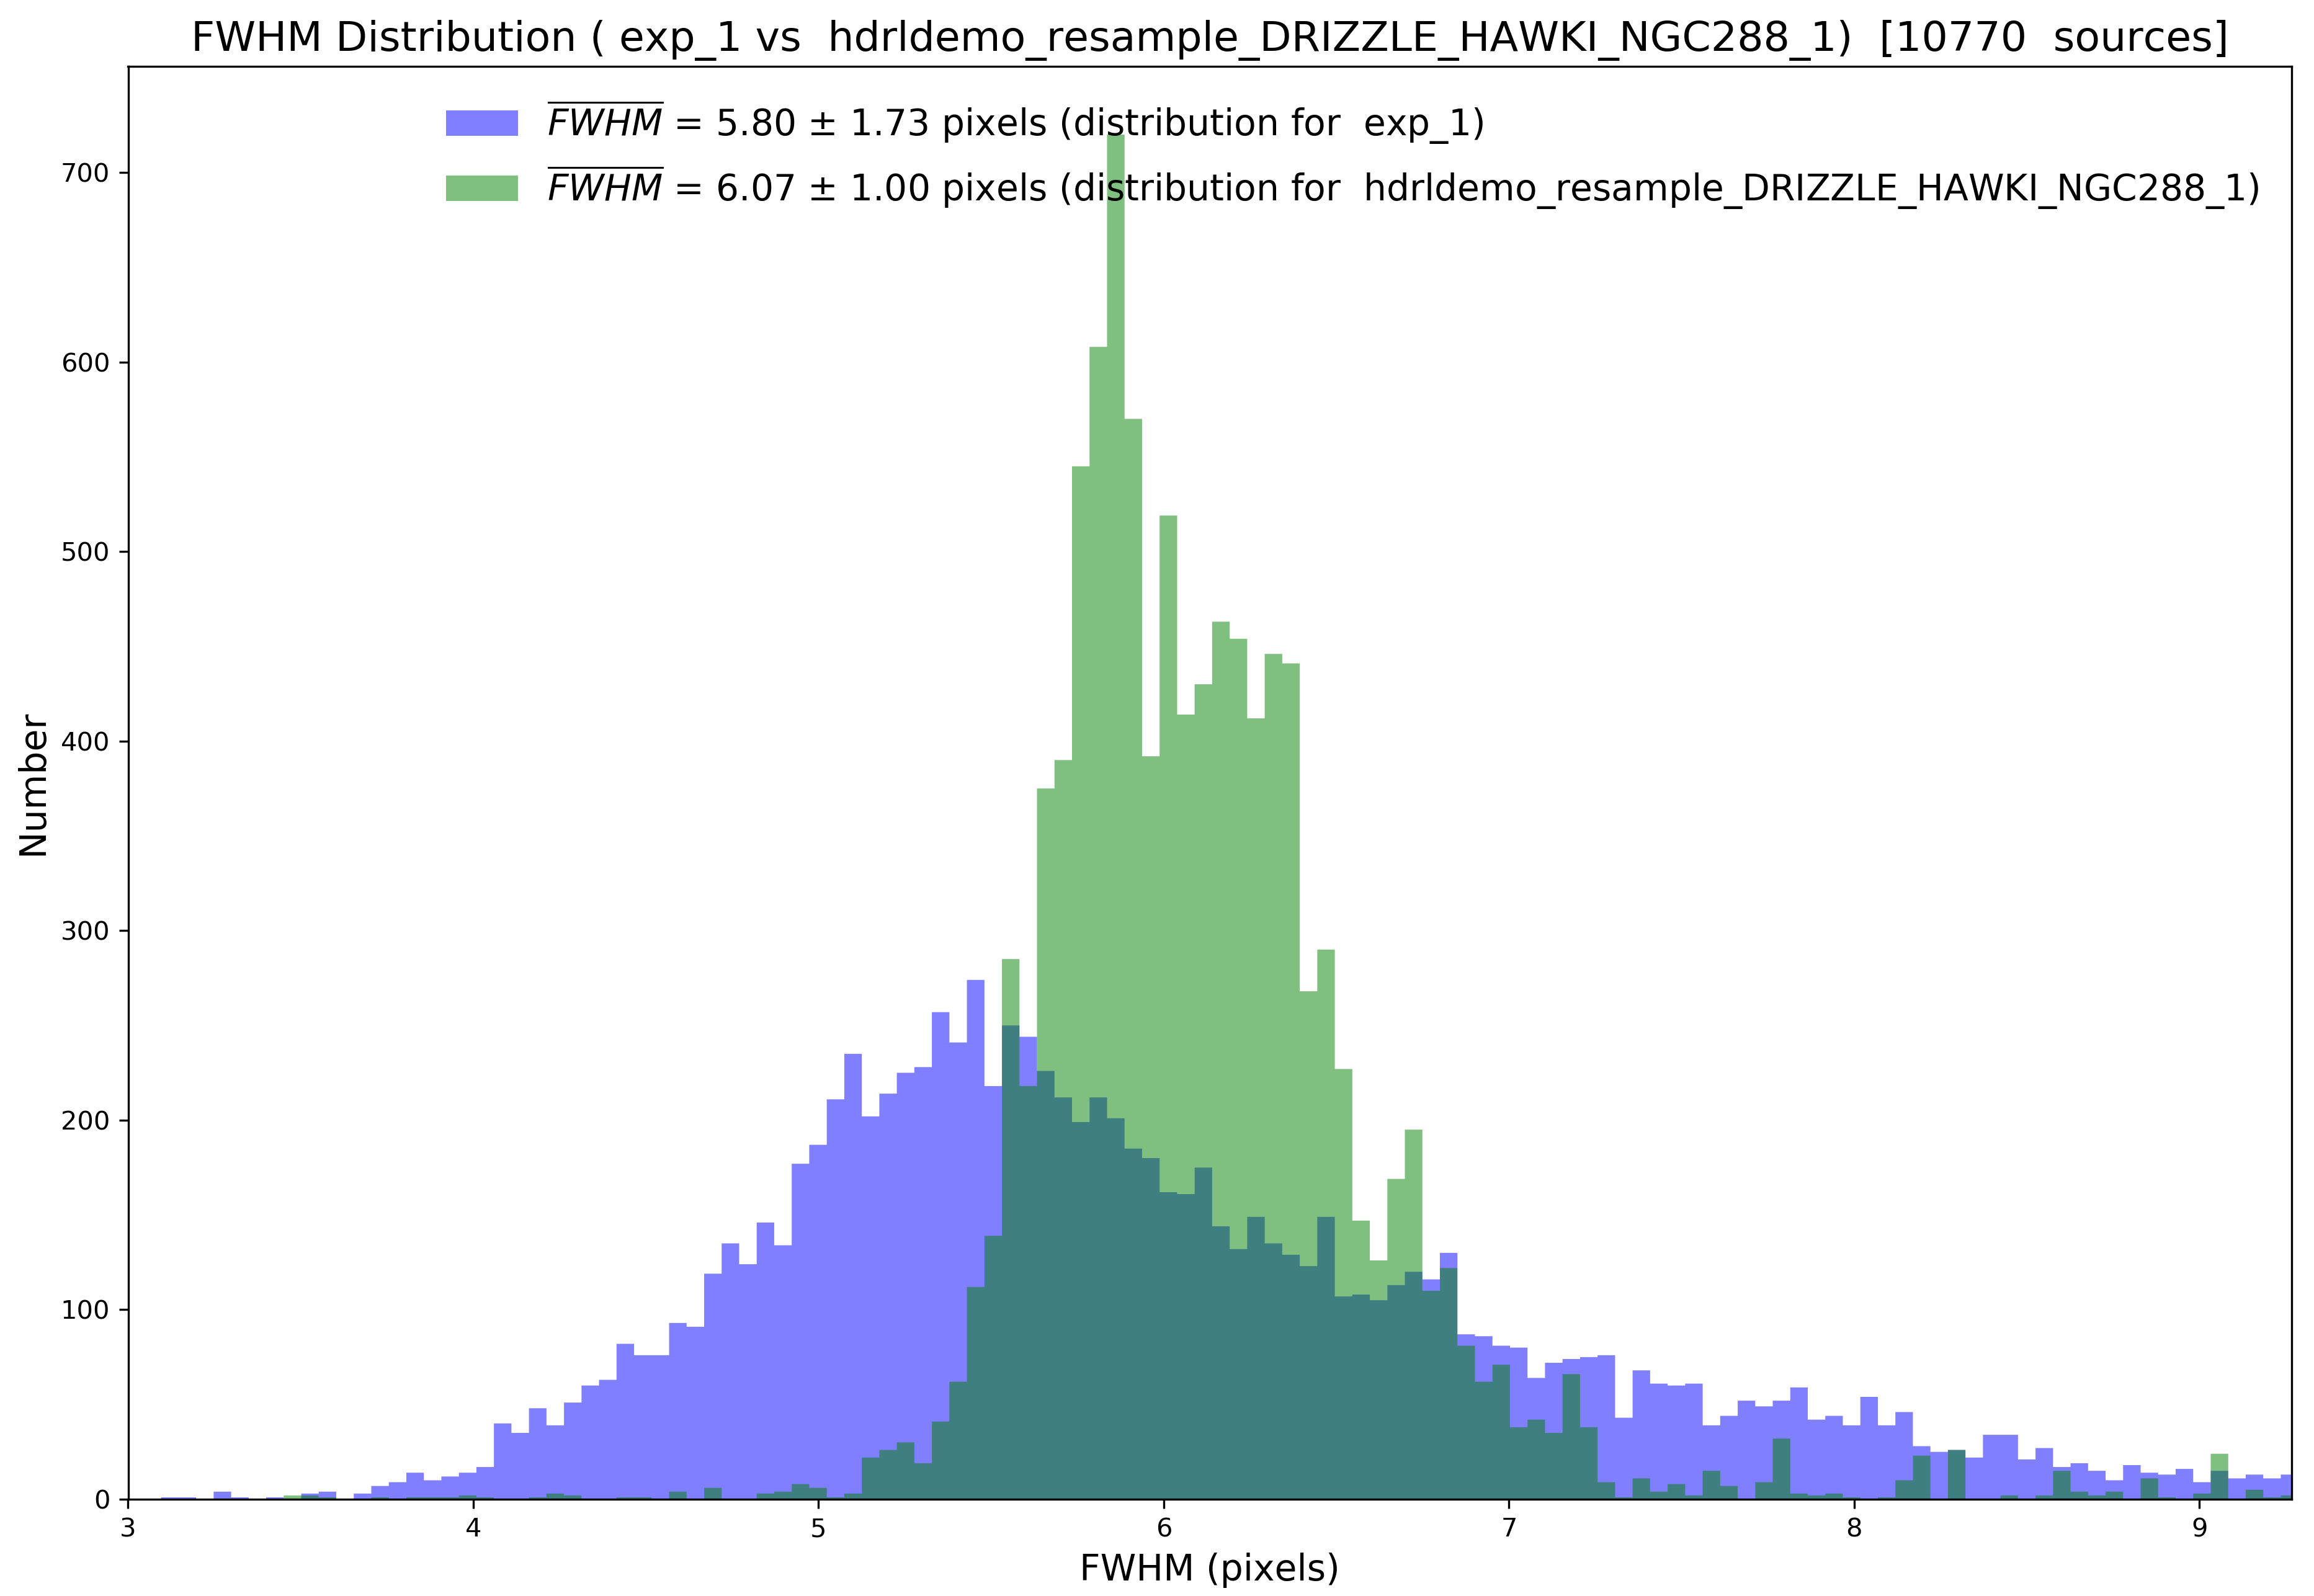
\includegraphics[width=8.4cm]{figures/match_field_DRIZZLE_HAWKI_NGC288_1_FWHM_histogram.png}
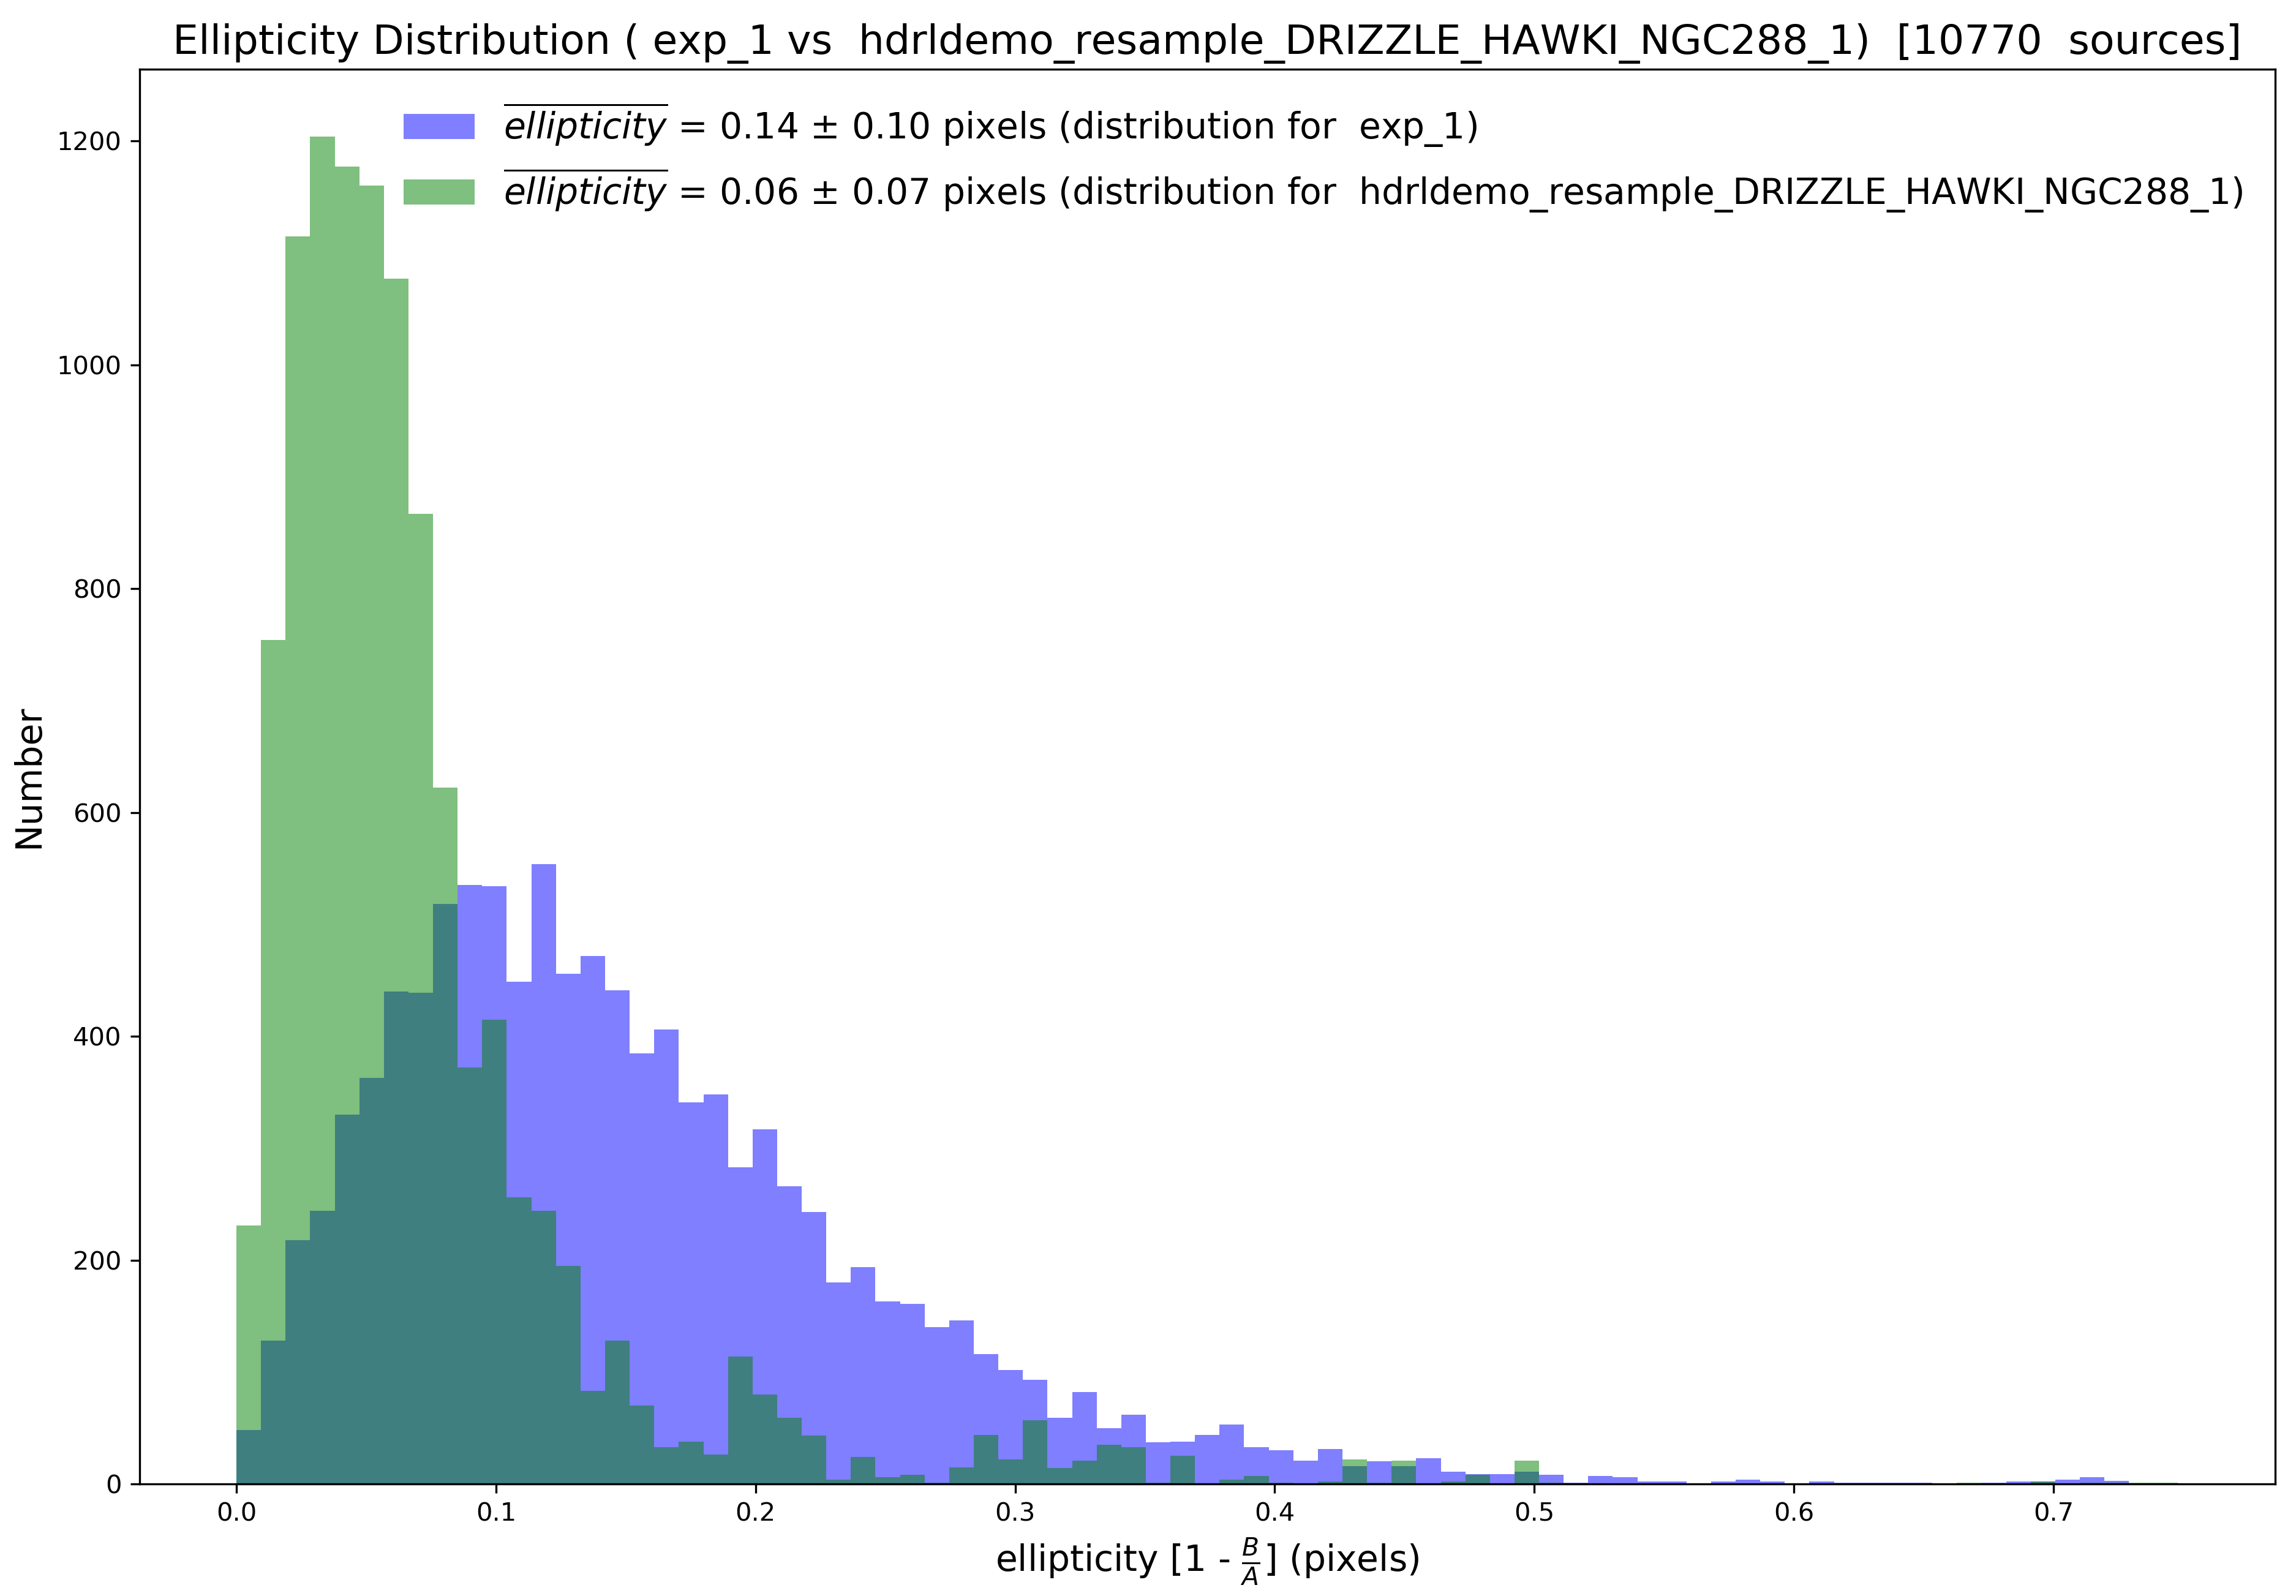
\includegraphics[width=8.4cm]{figures/match_field_DRIZZLE_HAWKI_NGC288_1_ellipticity_histogram.png} 
\caption[]
	{\footnotesize  A comparison of FWHM and ellipticity for the sources in the HAWK-I input images (blue histograms) and those
	after resampling (green histograms).  The resampling was done with {\tt --method=DRIZZLE} and {\tt --method.loop-distance=1}.\\
	{\bf left panel:}    The FWHM distribution of the 10,000 sources in the NGC288 field. As expected, the median FWHM, after resampling, increases slightly.  
	                           Since the increase in FWHM is less than 5\%, this is acceptable.\\
	{\bf right panel:} The distribution of ellipticities.   Here, the resampling has circularised the sources.   This, too, is as expected. 
	}
	\label{fig:fwhm_ellip_NGC288}
\end{figure}



%  
%  M30:
\subsubsection{M30}

The analysis of the denser globular cluster M30 shows similar good results when the individual input HAWK-I images are compared to the
resampled results.   An example of the \hdrlresample\ product ({\tt --method=DRIZZLE} and {\tt --method.loop-distance=1})
is shown in figure \ref{fig:hawki_M30}.  

\begin{figure}[H]
\centering
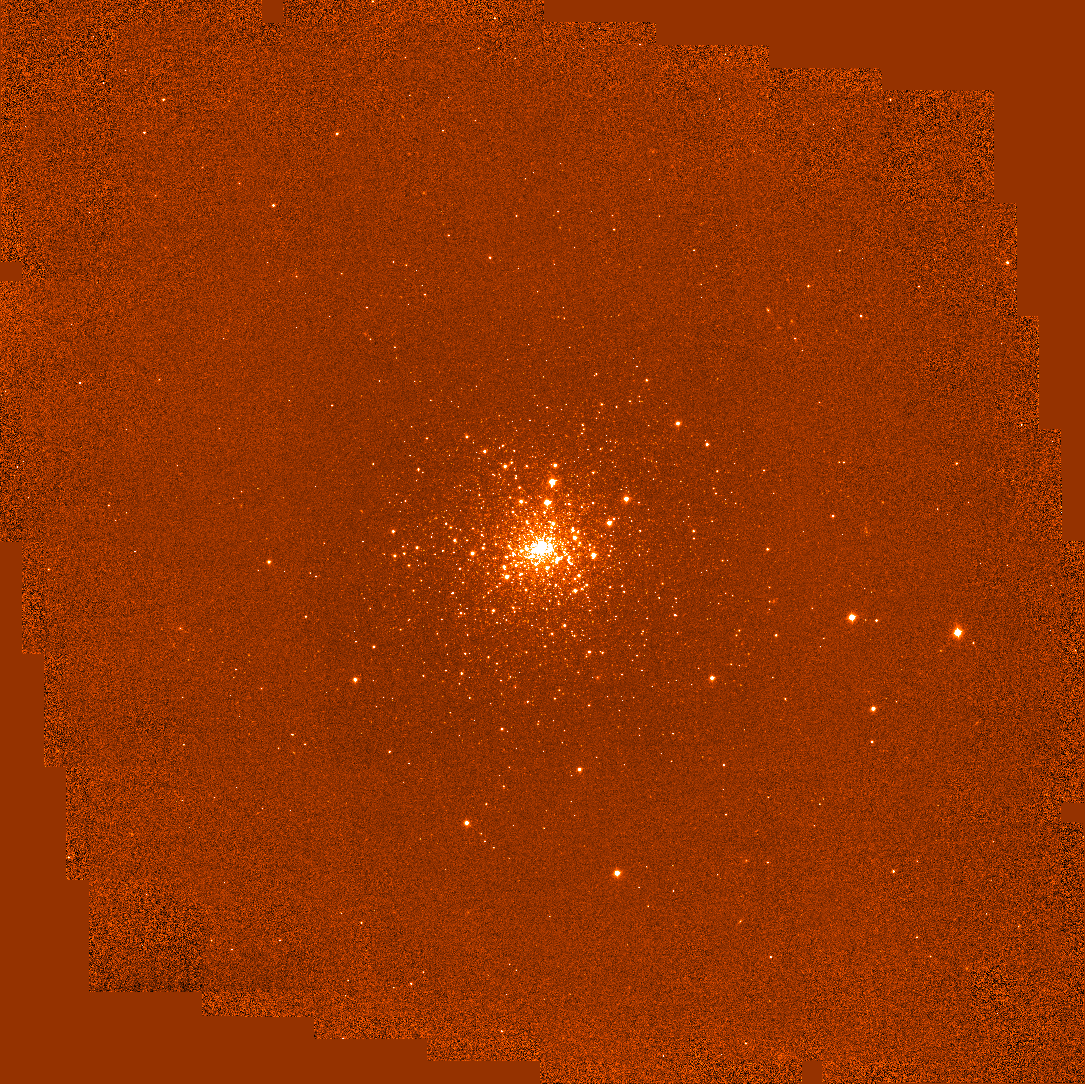
\includegraphics[width=8.4cm]{figures/Distortion_M30_TILED_IMAGE.png}
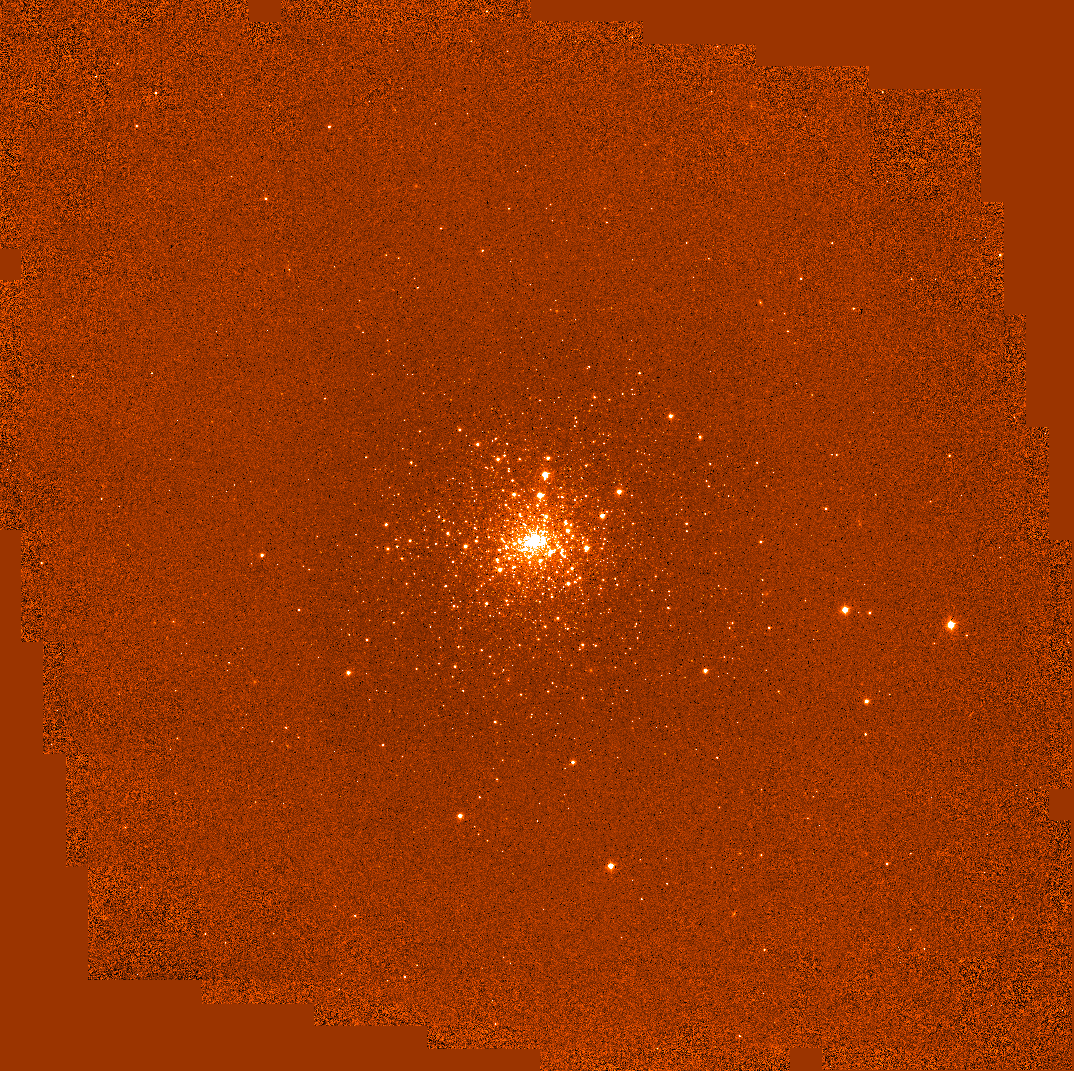
\includegraphics[width=8.4cm]{figures/hdrldemo_resample_DRIZZLE_HAWKI_M30_1.png} 
\caption[]
	{\footnotesize  The final tile image made from 100 HAWK-I images of the M30 field:\\
	{\bf left panel:}    as creating by the HAWK-I pipeline v. 2.4.6 routine {\tt hawki\_science\_postprocess}\\
	{\bf right panel:} as resampled and combined using \hdrlresample\ with {\tt --method=DRIZZLE} and {\tt --method.loop-distance=1}.\\
	}
	\label{fig:hawki_M30}
\end{figure}


As in the previous HAWK-I example, all five methods of image resampling retained the astrometric quality following interpolation.  This is evident in 
figure \ref{fig:radec_M30}.  Here, the absolute positions of the sources in the 100 input HAWK-I images is compared to the absolute positions
of the sources in the image resample using the {\tt QUADRATIC} method.   Here, the median $\Delta\alpha*\cos(\delta)=-0.002\pm0.11\ arcsec$ and 
$\Delta\delta=-0.007\pm0.12\ arcsec$ with the cloud of offsets spread symmetrically about the origin.  
Considering that the HAWK-I pixel size is 0.106 pixels/arcsec, the standard deviation of the astrometric accuracy approximately one pixel.

\begin{figure}[H]
\centering
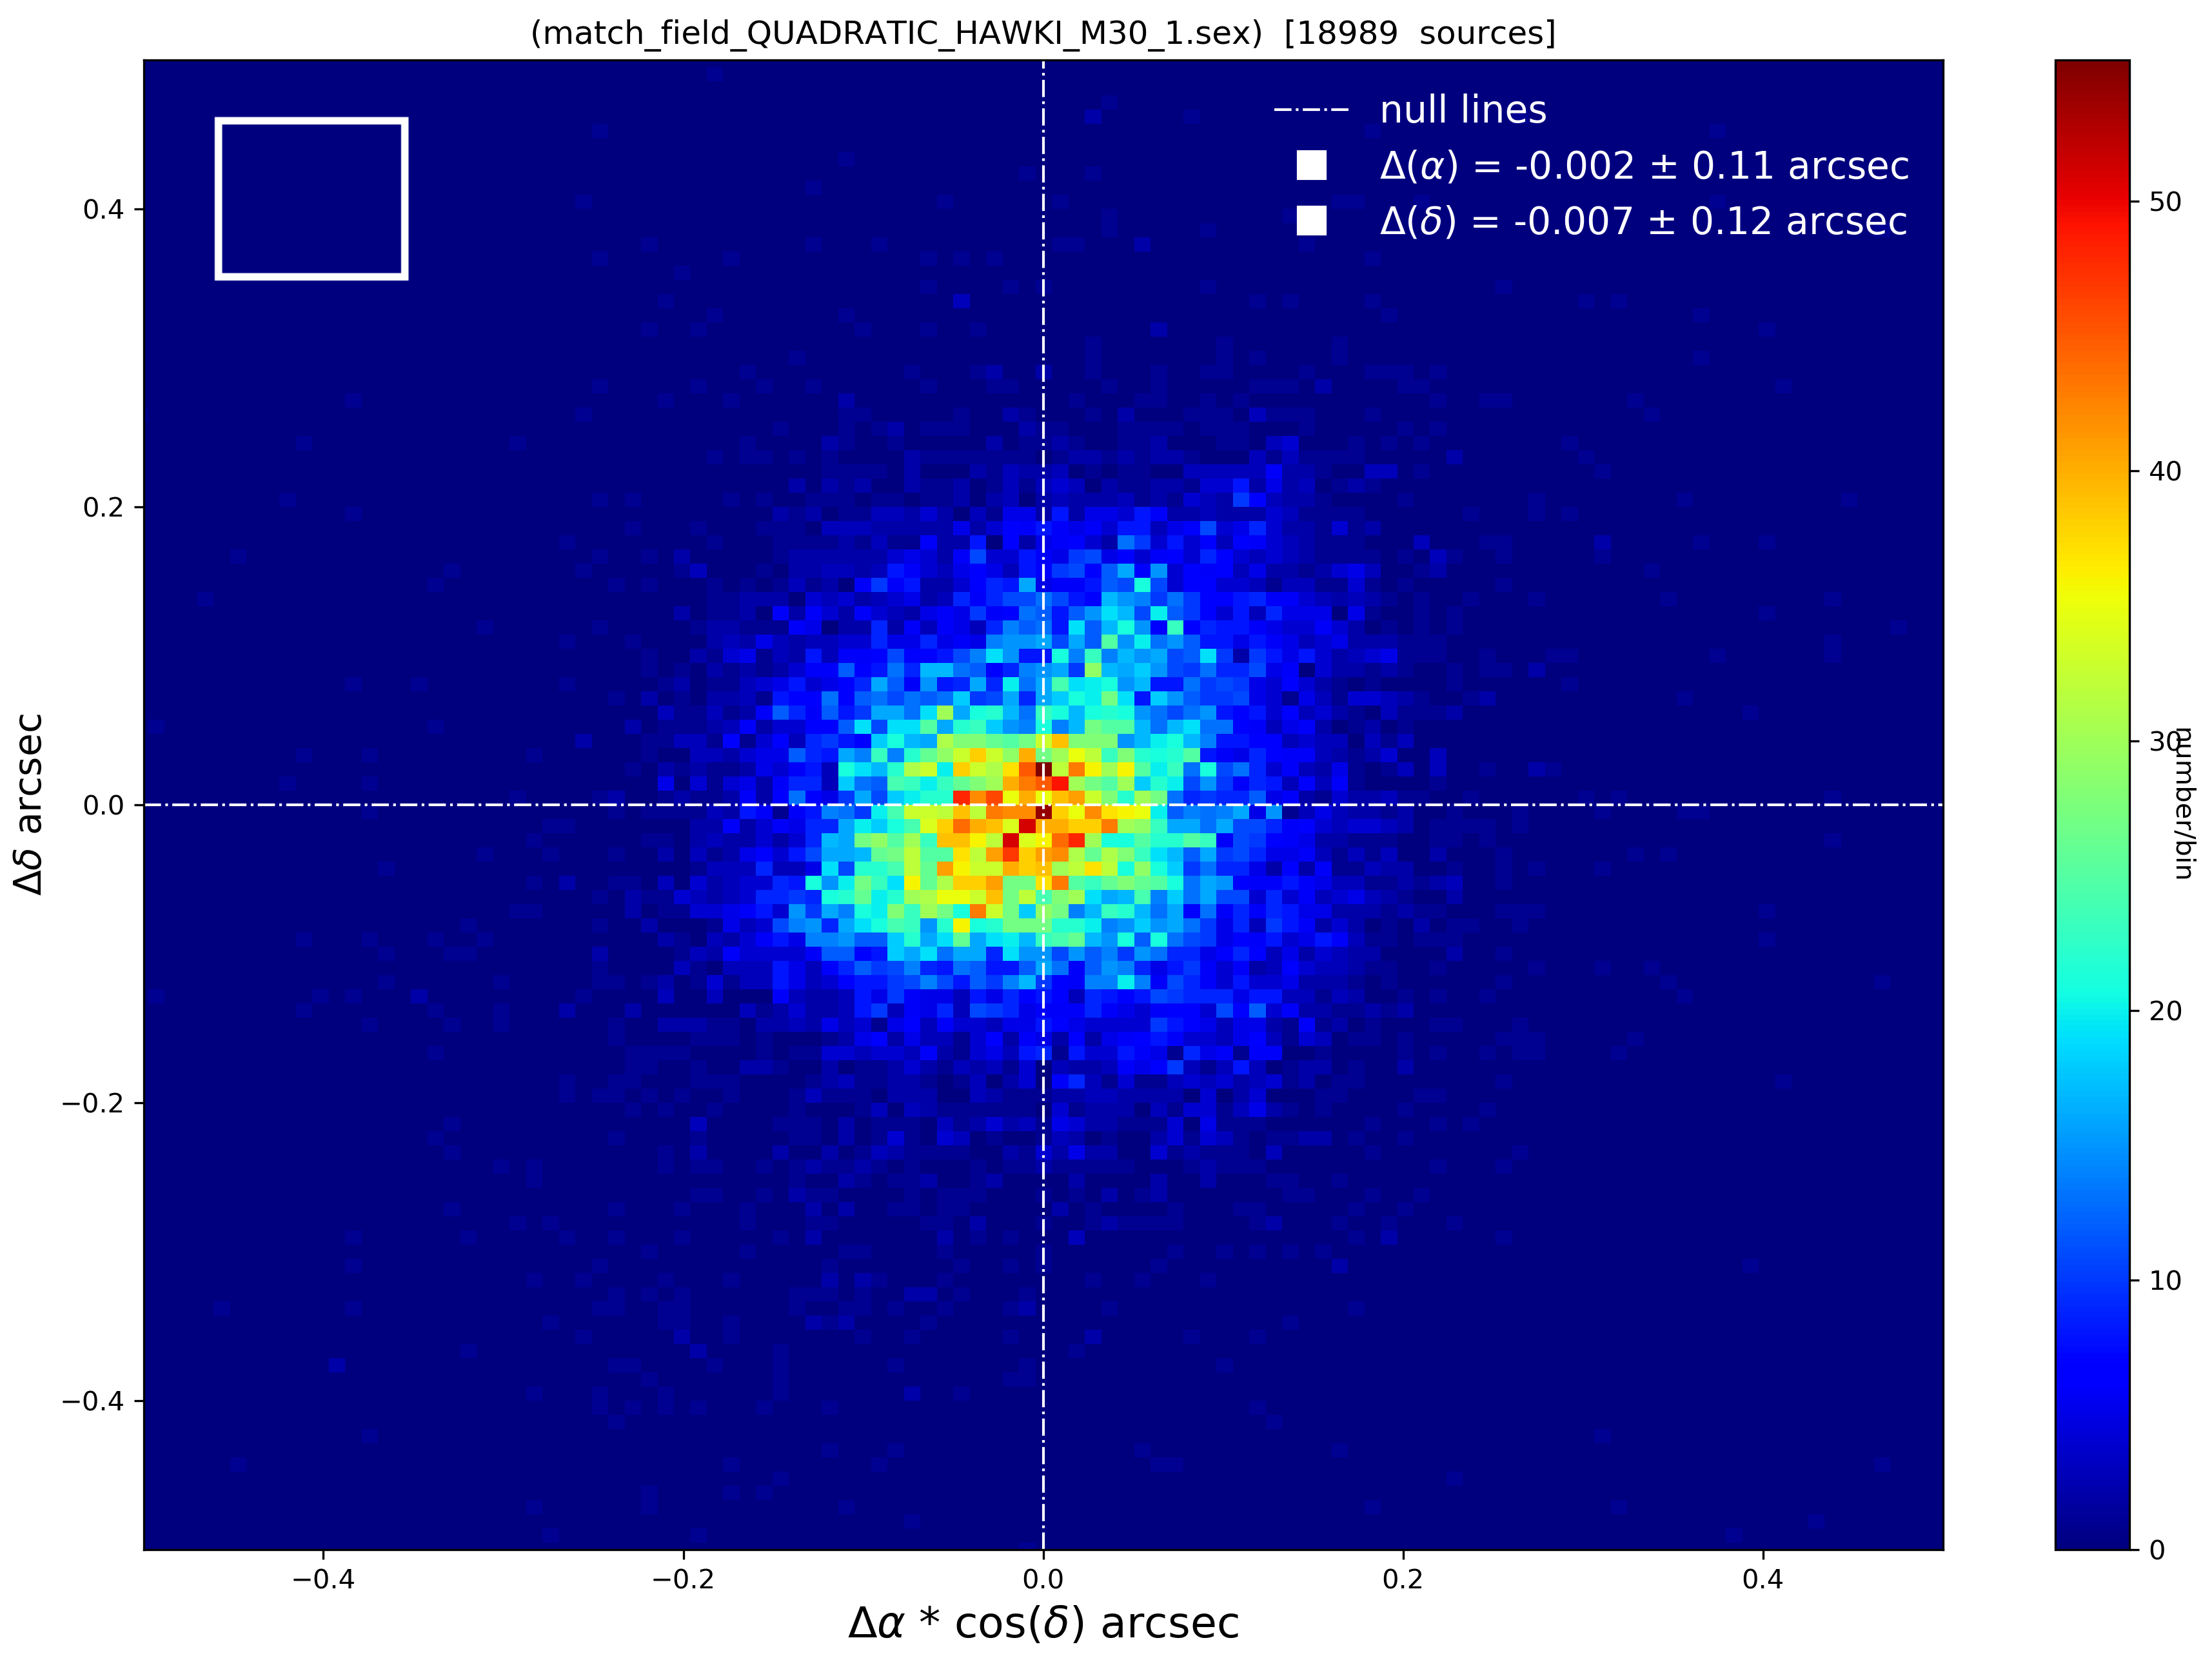
\includegraphics[width=11cm]{figures/match_field_QUADRATIC_HAWKI_M30_1_RA_DEC_scatter_plot.png}
\caption[]
	{\footnotesize  the astrometric quality of the \hdrlresample\ routines as measured by comparing almost 19,000 sources in the original input HAWK-I images
	with those in the resampled ({\tt QUADRATIC}) image tile of Figure \ref{fig:hawki_M30}.
	The standard deviation of the $\Delta\alpha*\cos(\delta)$ and $\Delta\delta$ distributions is 0.12 arcsec. This is approximately the size of one HAWK-I
	pixel (0.106 pixels/arcsec).  The pixel size is indicated by the white square in the top left corner.
	}
	\label{fig:radec_M30}
\end{figure}

Similarly, the photometric quality is also retained following interpolation.   Figure \ref{fig:mag_M30} is typical of all interpolated frames, with a source magnitude match 
between the individual HAWK-I images and the resampled ({\tt LANCZOS}) image tile of $\Delta(mag)=-0.023\pm0.08$ magnitudes.

\begin{figure}[H]
\centering
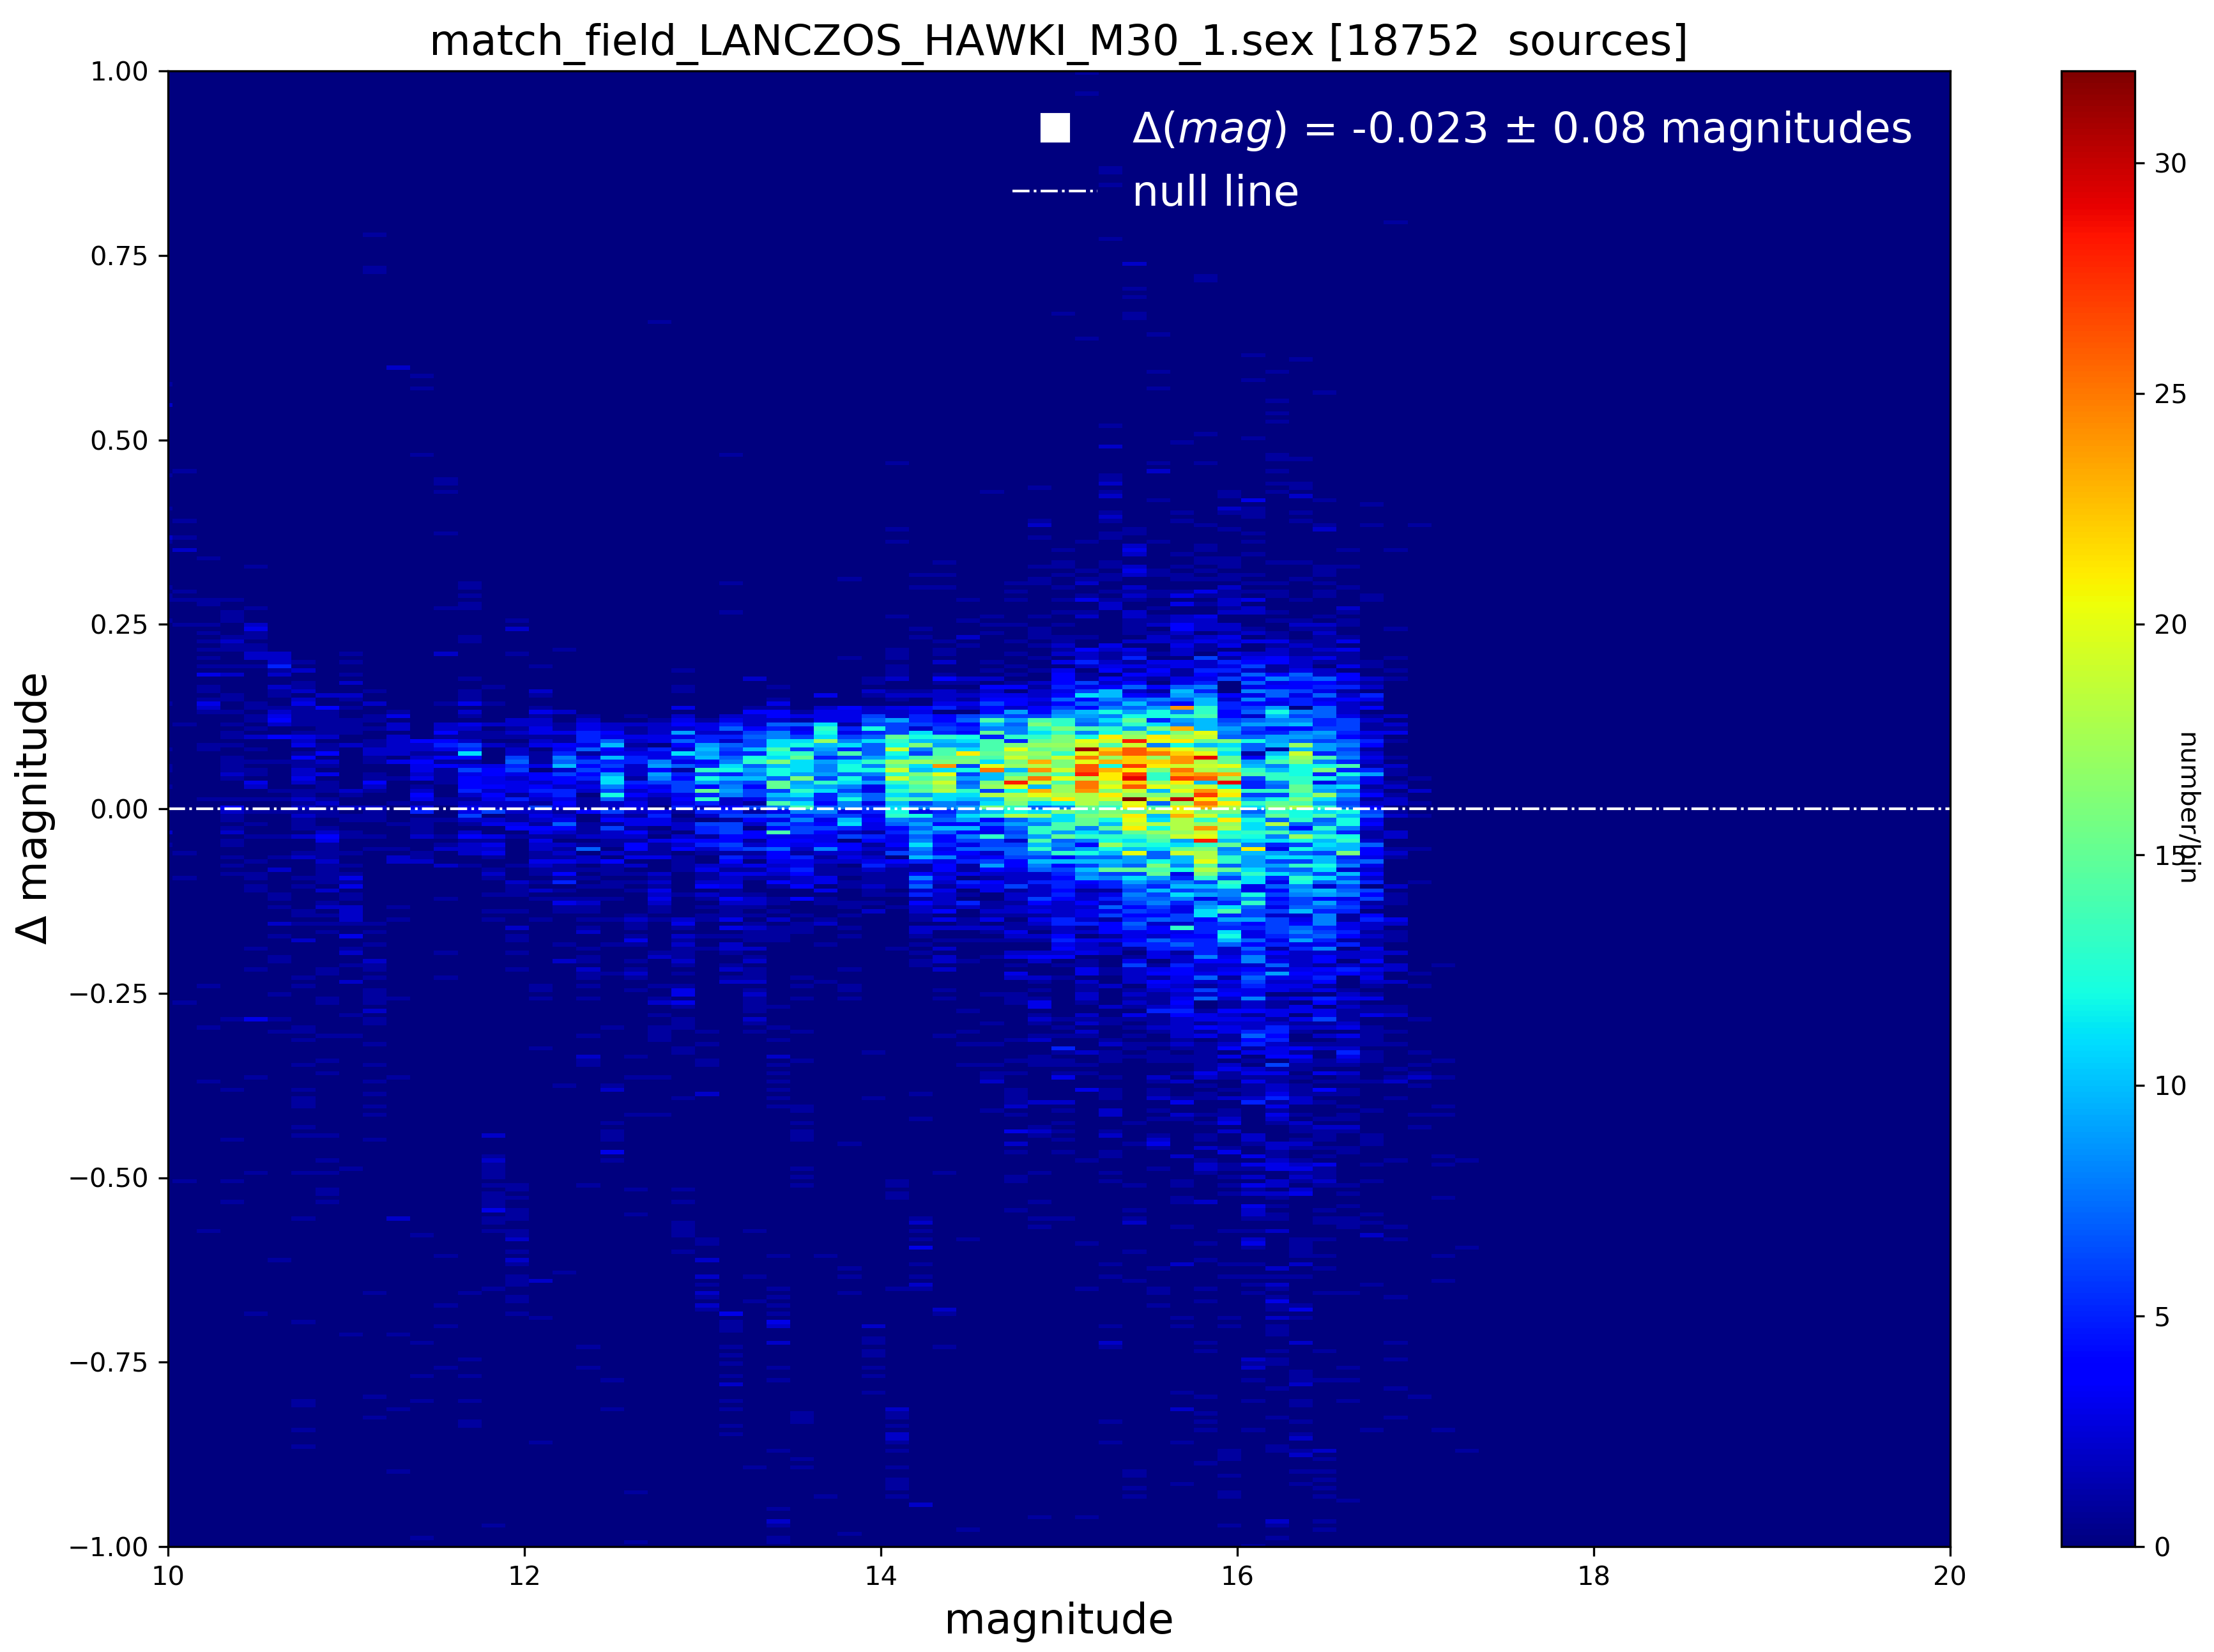
\includegraphics[width=11cm]{figures/match_field_LANCZOS_HAWKI_M30_1_mag_scatter_plot.png}
\caption[]
	{\footnotesize  the photometric quality of the \hdrlresample\ routines as measured by comparing the more than 18,000 sources in the original input HAWK-I images
	with those in the resampled ({\tt LANCZOS}) image tile of Figure \ref{fig:hawki_M30} (right panel).
	The standard deviation of the $\Delta(mag)$  distribution is 0.08 magnitudes. 	
	}
	\label{fig:mag_M30}
\end{figure}

As can be seen in figure \ref{fig:fwhm_ellip_M30}, the resampling causes a slight increase in the FWHM of the sources and a decrease in the source ellipticities.
This is expected, since the resampling will cause a circularisation and homogenisation of the source shapes.


\begin{figure}[H]
\centering
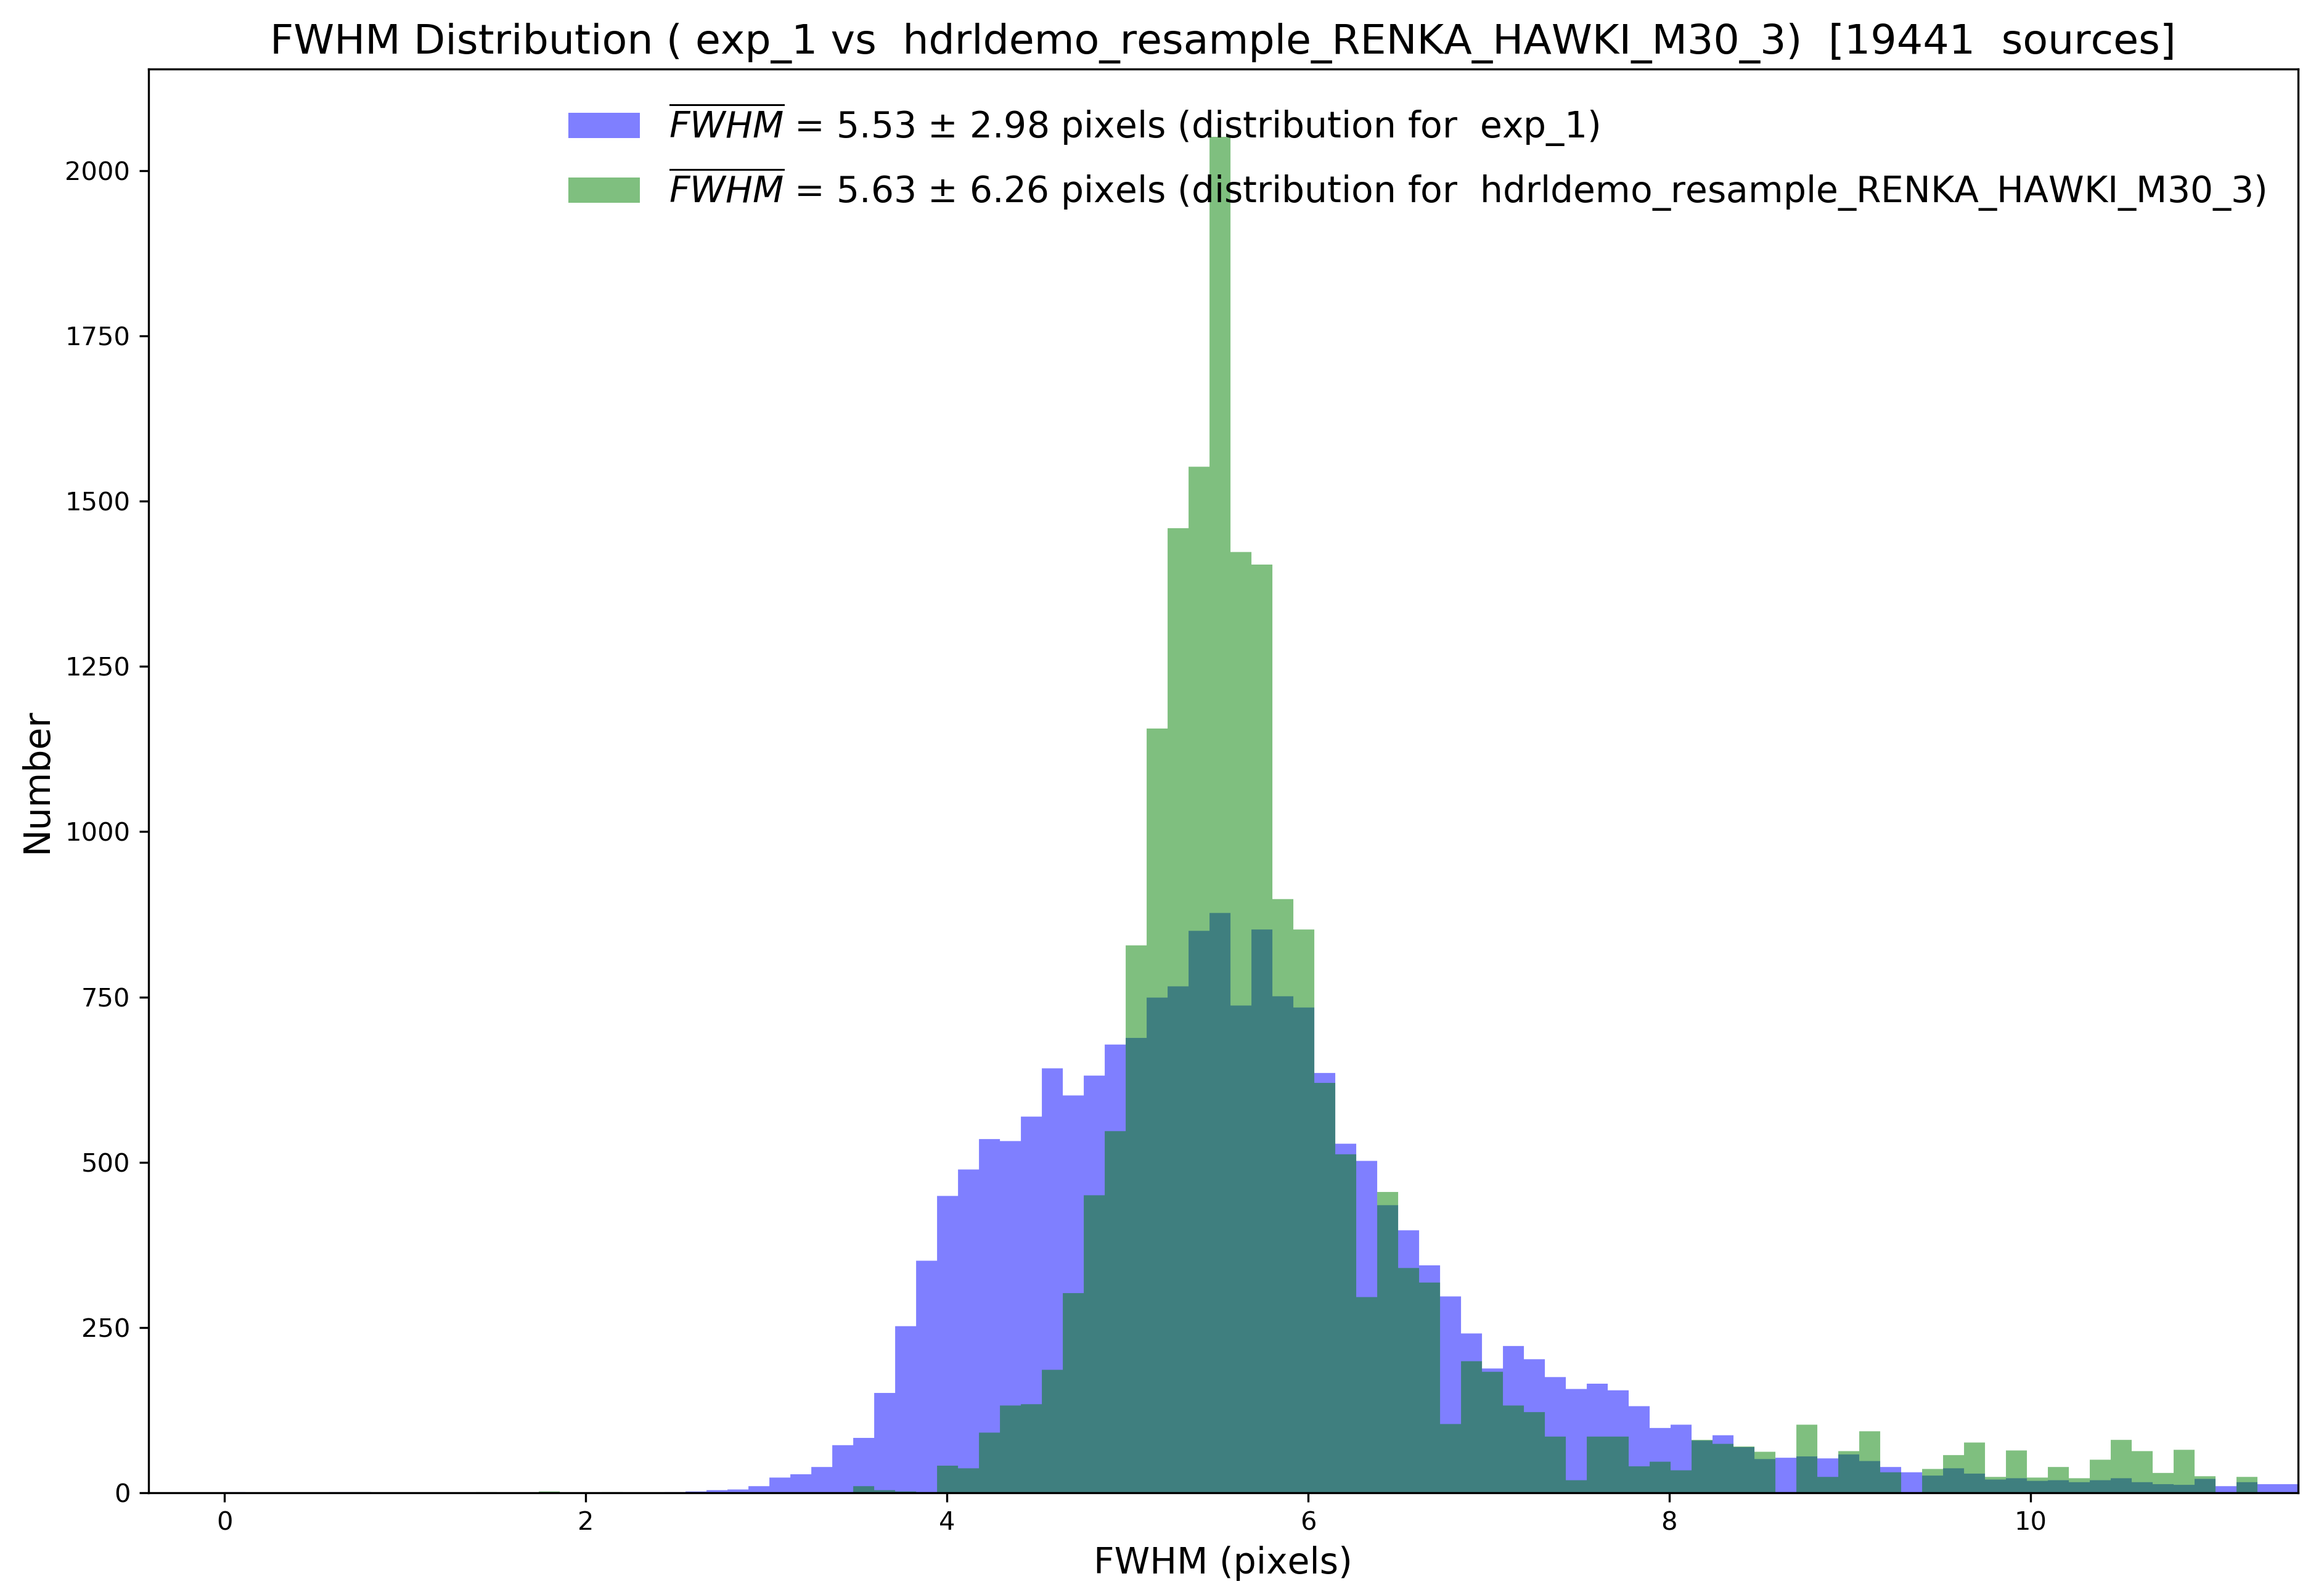
\includegraphics[width=8.4cm]{figures/match_field_RENKA_HAWKI_M30_3_FWHM_histogram.png}
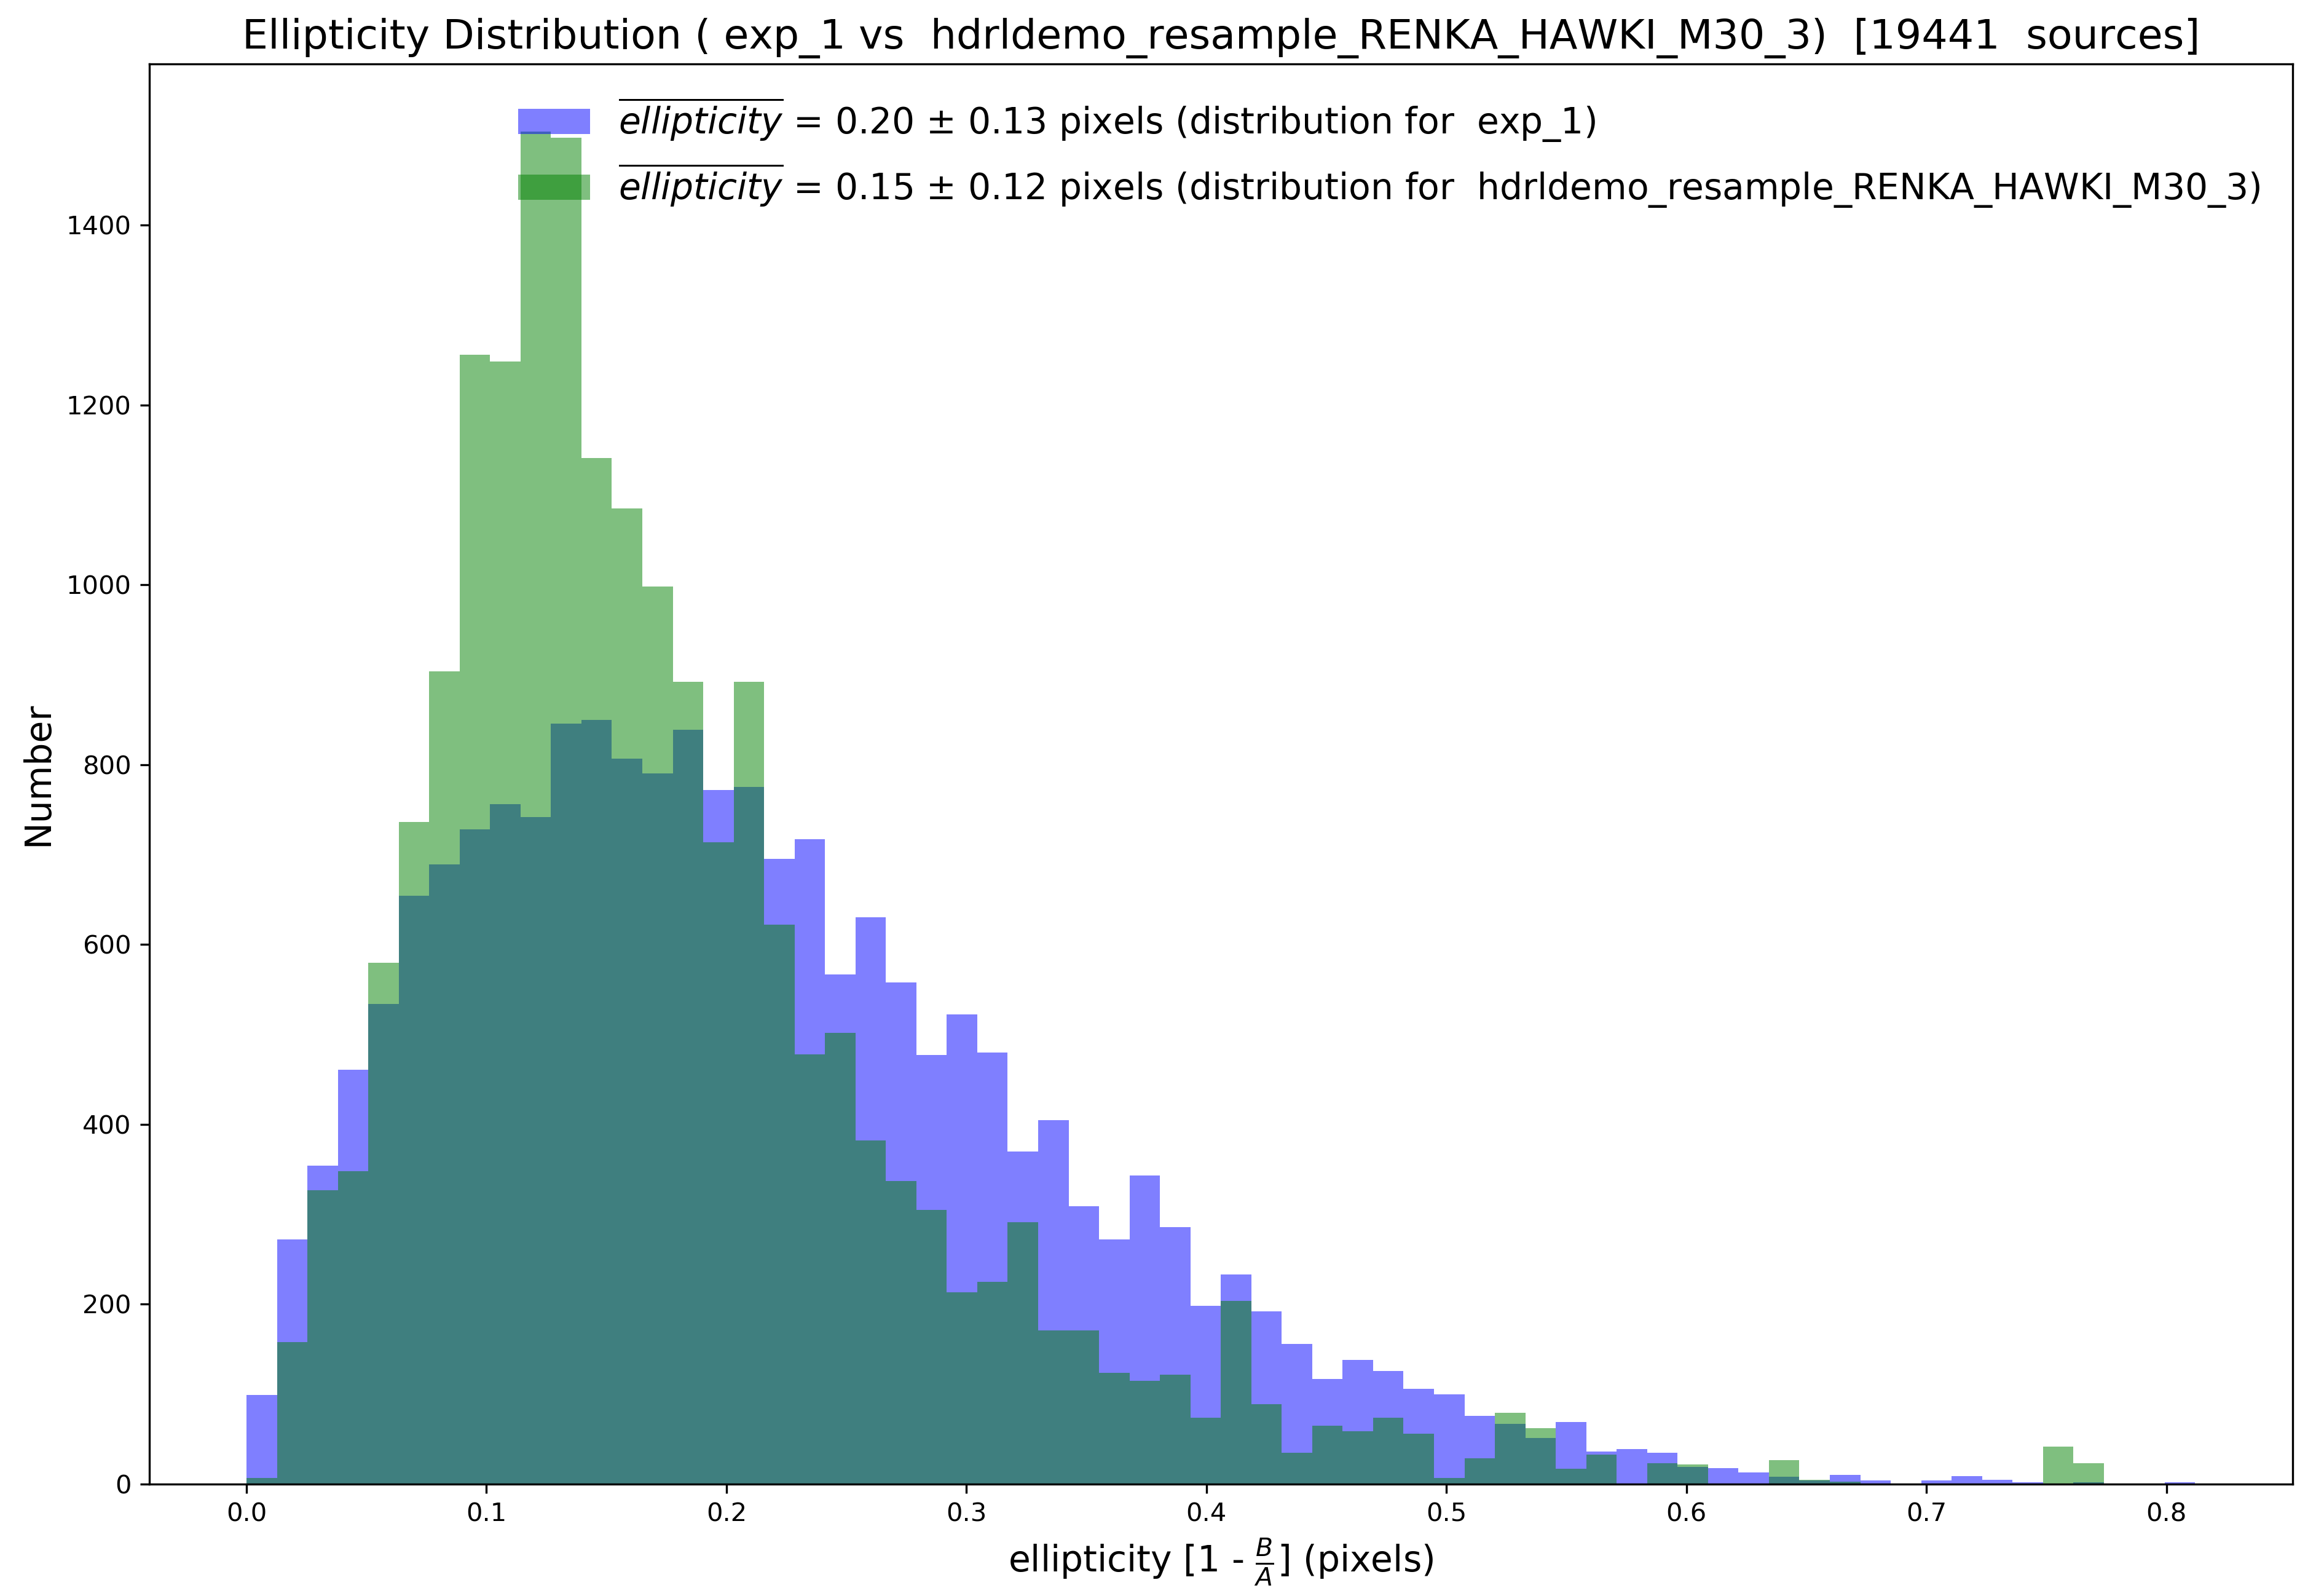
\includegraphics[width=8.4cm]{figures/match_field_RENKA_HAWKI_M30_3_ellipticity_histogram.png} 
\caption[]
	{\footnotesize  A comparison of FWHM and ellipticity for the sources in the HAWK-I input images (blue histograms) and those
	after resampling (green histograms).  The resampling was done with {\tt --method=RENKA} and {\tt --method.loop-distance=3}.\\
	{\bf left panel:}    The FWHM distribution of the 19,441 sources in the M30 field. As expected, the median FWHM, after resampling, increases slightly.  
	                           Since the increase in FWHM is less than 5\%, this is acceptable.\\
	{\bf right panel:} The distribution of ellipticities.   Here, the resampling has circularised the sources.   This, too, is as expected. 
	}
	\label{fig:fwhm_ellip_M30}
\end{figure}



A summary of the source attributes between the input frames and the resampled images is given in Table \ref{tab:compare_NGC288}.


\begin{sidewaystable}

\caption{A Summary of Comparisons Between Input HAWK-I Cluster Data Images and Resultant Interpolation Images}

\begin{center}
\begin{tabular}{|l|l|c|c|c|c|c|c|c|c|c|c|}                      
\toprule

Image         				     		     & Interpolation	 & N$_{frames}^2$   & Nmatch & $\Delta\alpha$  & $\Delta\delta$ &  $\Delta(mag)$ & $\sigma\Delta(mag)$ & FWHM1$^3$  & FWHM2$^4$  & ellip1$^3$  & ellip2$^4$  \\
                                     & method (LD)$^1$ &                         &               & (arcsec)            & (arcsec)          &                          &                                   & (pixels)    & (pixels)   &            & \\
\midrule
NGC\,288         & DRIZZLE (1)        & 100   	& 10,770 	& 0.001       &  0.003  	& -0.021 & 0.05          & 5.80  	& 6.07		& 0.14    & 0.06   \\
 	   	       	& DRIZZLE (3)        & 100  	& 10,770 	& 0.001       &  0.003  	& -0.021 & 0.05 	  & 5.80  	& 6.07  		& 0.14    & 0.06  \\
 	               	& LANCZOS (1)      & 100  	& 10,768 	& 0.001       &  0.003  	& -0.025 & 0.05          & 5.80  	& 6.01  		& 0.14    & 0.05    \\
 	   	      	& LANCZOS (3)      & 100  	& 10,760 	& 0.000       &  0.003  	& -0.029 & 0.05          & 5.80  	& 5.93  		& 0.14    & 0.05    \\
 	              	& LINEAR (1)          & 100    	& 10,794 	& 0.002       &  0.003  	& -0.012 & 0.05          & 5.80  	& 6.33  		& 0.14    & 0.06    \\
 	              	& LINEAR (3)          & 100    	& 10,782 	& 0.003       &  0.004  	&  0.015 & 0.06          & 5.80  	& 7.56  		& 0.14    & 0.06    \\
 	              	& NEAREST (1)      & 100   	& 9,879 	& -0.001       & 0.002  	& -0.044 & 0.06          & 5.80  	& 5.82  		& 0.13    & 0.12    \\
 	              	& NEAREST (3)      & 100   	& 9,879 	& -0.001       & 0.002  	& -0.044 & 0.06          & 5.80  	& 5.82  		& 0.13    & 0.12    \\
 	              	& QUADRATIC (1)  & 100 	& 10,739 	& 0.001        & 0.004  	& -0.023 & 0.05          & 5.80  	& 6.14  		& 0.14    & 0.06    \\
 	              	& QUADRATIC (3)  & 100 	& 10,724 	& 0.002        & 0.004  	& -0.015 & 0.05          & 5.80  	& 6.52   		& 0.14    & 0.06    \\
 	              	& RENKA (1)           & 100 	& 10,718 	& 0.000        & 0.004  	& -0.030 & 0.05          & 5.80  	& 6.04 		& 0.14    & 0.07    \\
                		& RENKA (3)           & 100  	& 10,718 	& 0.000        & 0.004  	& -0.030 & 0.05          & 5.80  	& 6.04  		& 0.14    & 0.07    \\
\midrule
M\,30         	& DRIZZLE (1)        & 100   	& 18,678 	& -0.002       & -0.006  	& -0.020 & 0.08          & 5.51    & 5.53  		& 0.19    & 0.14    \\
 	   	       	& DRIZZLE (3)        & 100  	& 18,678 	& -0.002       & -0.006  	& -0.020 & 0.08 	 & 5.51    & 5.53  		& 0.19    & 0.14  \\
 	               	& LANCZOS (1)      & 100  	& 18,752 	& -0.002       & -0.007  	& -0.023 & 0.08          & 5.51    & 5.49  		& 0.19    & 0.14    \\
 	   	      	& LANCZOS (3)      & 100  	& 18,852 	& -0.002       & -0.006  	& -0.026 & 0.08          & 5.51    & 5.42  		& 0.19    & 0.14    \\
 	              	& LINEAR (1)          & 100    	& 18,187 	& -0.002       & -0.005  	& -0.008 & 0.09          & 5.50    & 5.77  		& 0.19    & 0.13    \\
 	              	& LINEAR (3)          & 100    	& 16,999 	& -0.001       & -0.004 	&  0.025 & 0.09          & 5.50    & 6.97 		& 0.19    & 0.13    \\
 	              	& NEAREST (1)      & 100   	& 19,189 	& -0.006       & -0.004 	& -0.052 & 0.11          & 5.59    & 5.75  		& 0.20    & 0.21    \\
 	              	& NEAREST (3)      & 100   	& 19,189 	& -0.006       & -0.004  	& -0.052 & 0.11          & 5.59    & 5.75  		& 0.20    & 0.21    \\
 	              	& QUADRATIC (1)  & 100 	& 18,989 	& -0.002       & -0.007  	& -0.026 & 0.09          & 5.52    & 5.66  		& 0.19    & 0.14    \\
 	              	& QUADRATIC (3)  & 100 	& 18,499 	& -0.003       & -0.005  	& -0.016 & 0.09          & 5.51    & 5.97   		& 0.19    & 0.13     \\
 	              	& RENKA (1)           & 100 	& 19,413 	& -0.003       & -0.007  	& -0.034 & 0.09          & 5.53    & 5.63 		& 0.20    & 0.15    \\
                		& RENKA (3)           & 100  	& 19,441 	& -0.003       & -0.007  	& -0.034 & 0.09          & 5.53    & 5.63  		& 0.20    & 0.15    \\
\bottomrule


\end{tabular}	
\end{center}																											

\label{tab:compare_NGC288}
\noindent{
		$^1$ The interpolation method and loop-distance used ({\tt --method.loop-distance}).\\
		$^2$ The total number of synthetic input images combined during the resampling.\\
		$^3$ FWHM1 and ellip1 refer to the individual, HAWK-I input images.\\
		$^4$ FWHM2 and ellip2 refer to the resampled images.}
	\end{sidewaystable}




  
\subsection{Results from Strongly Rotated HAWK-I Images}
\label{sect:hawki2}

In order to test for any flexure in the HAWK-I instrument, an observing block (OB) was designed that allows the camera co-rotator to
travel through 160$^\circ$ while pointing at the same field of view.   This data set was obtained on the night of 2015-08-28 and has
programme id {\tt 60.A-9283(A)} and the observing block id {\tt 200346422}.  It consists of 20 separate exposures of four detectors, with each
pair of images rotated by 20$^\circ$ for a total of 160$^\circ$.   Clearly, a complex data set consisting of 80 distinct detector frames with such
a large overall rotation is an ideal stress test in order to see how well the \hdrlresample\ routines perform.
 
 \begin{figure}[ht]
\centering
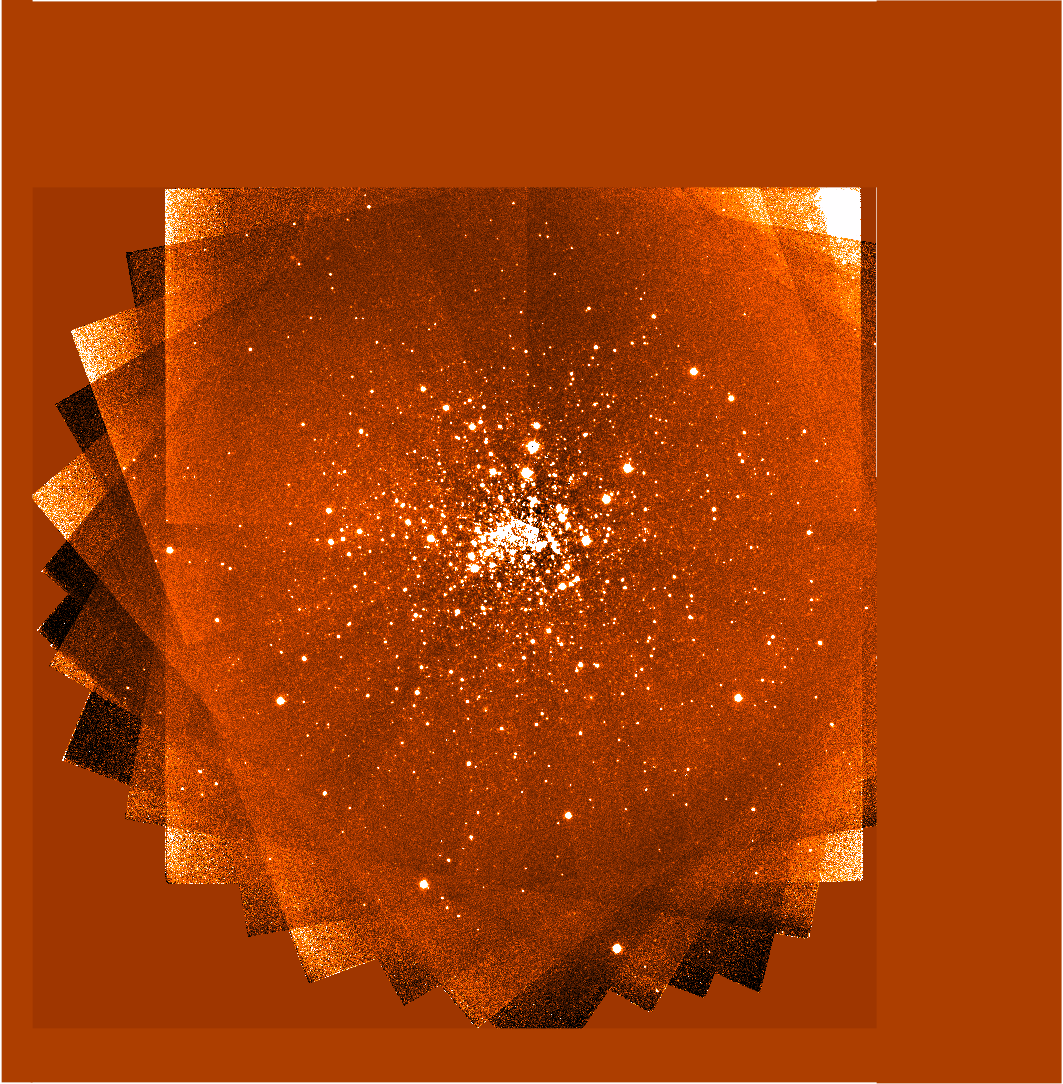
\includegraphics[width=8.4cm]{figures/Flexure_M30_TILED_IMAGE.png}
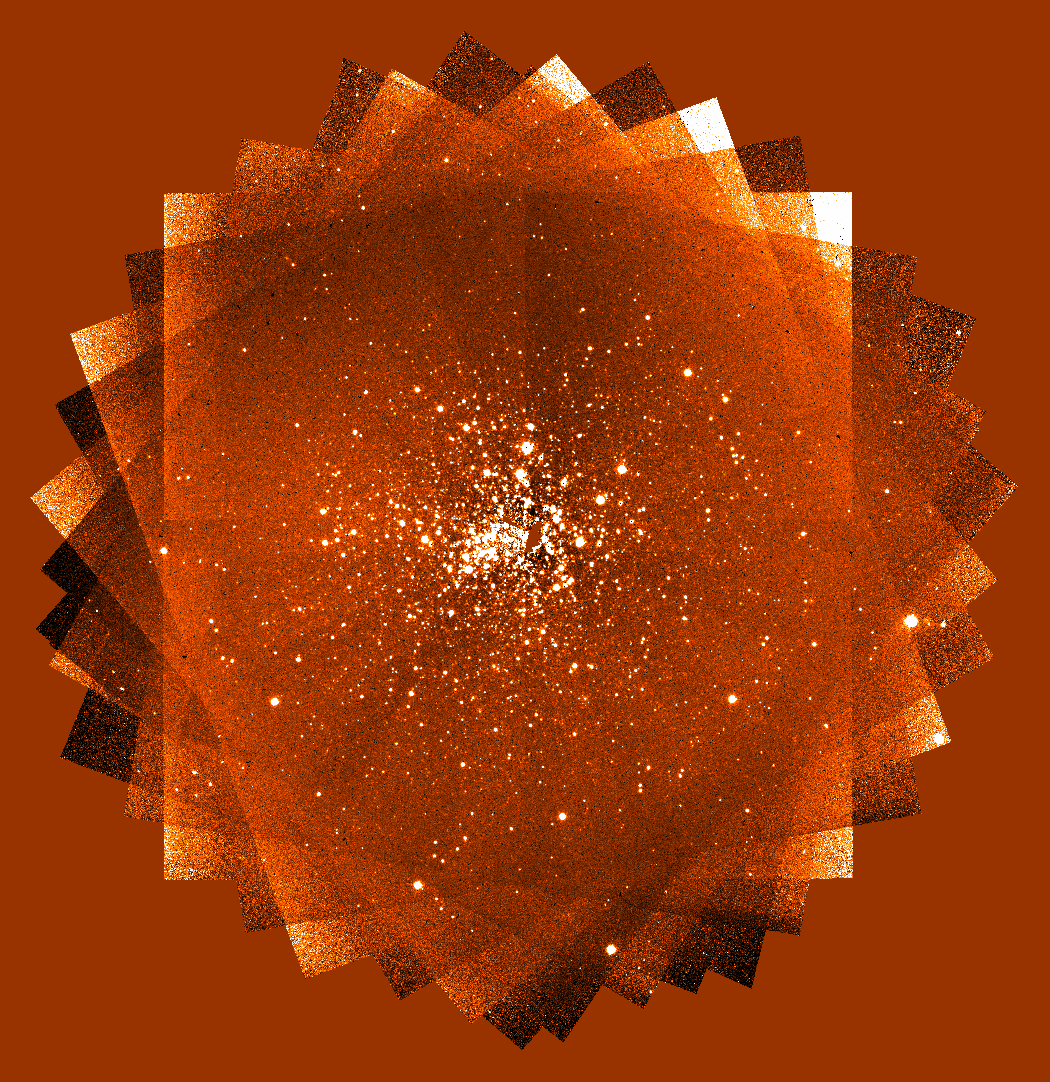
\includegraphics[width=8.4cm]{figures/hdrldemo_resample_DRIZZLE_HAWKI_rotation_1.png} 
\caption[]
	{\footnotesize  The final tile image made from 80 HAWK-I flexure frames:\\
	{\bf left panel:}    Creating by the HAWK-I pipeline v. 2.4.6 routine {\tt hawki\_science\_postprocess}\\
	{\bf right panel:} Resampled and combined using \hdrlresample\ with {\tt --method=DRIZZLE} and {\tt --method.loop-distance=1}.\\
	The only major difference between the two images is that the HAWK-I pipeline trims the tile, whereas \hdrlresample\ creates the a maximal
	area occupied by the WCS from all input images.
	}
	\label{fig:hawki_flexure}
\end{figure}

The 20 $\times$ 4 separate exposures were resampled using each of the methods available in \hdrlresample, {\tt NEAREST, LINEAR, QUADRATIC, RENKA, LANCZOS,
and DRIZZLE}, each with a loop distance of 1 and 3 pixels.   The resulting image tiles were then compared to the tile resulting from processing the identical
data with the HAWK-I pipeline version 2.4.6.

As in the previous HAWK-I example, all five methods of image resampling retained the astrometric quality following interpolation.  This is evident in 
figure \ref{fig:radec_flexure}.  Here, the absolute positions of the sources in the 80 input HAWK-I images is compared to the absolute positions
of the sources in the image resample using the {\tt LINEAR} method.   Here, the median $\Delta\alpha*\cos(\delta)=-0.004\pm0.13\ arcsec$ and 
$\Delta\delta=-0.011\pm0.14\ arcsec$ with the cloud of offsets spread symmetrically about the origin.  
Considering that the HAWK-I pixel size is 0.106 pixels/arcsec, the standard deviation of the astrometric accuracy approximately one pixel.

\begin{figure}[H]
\centering
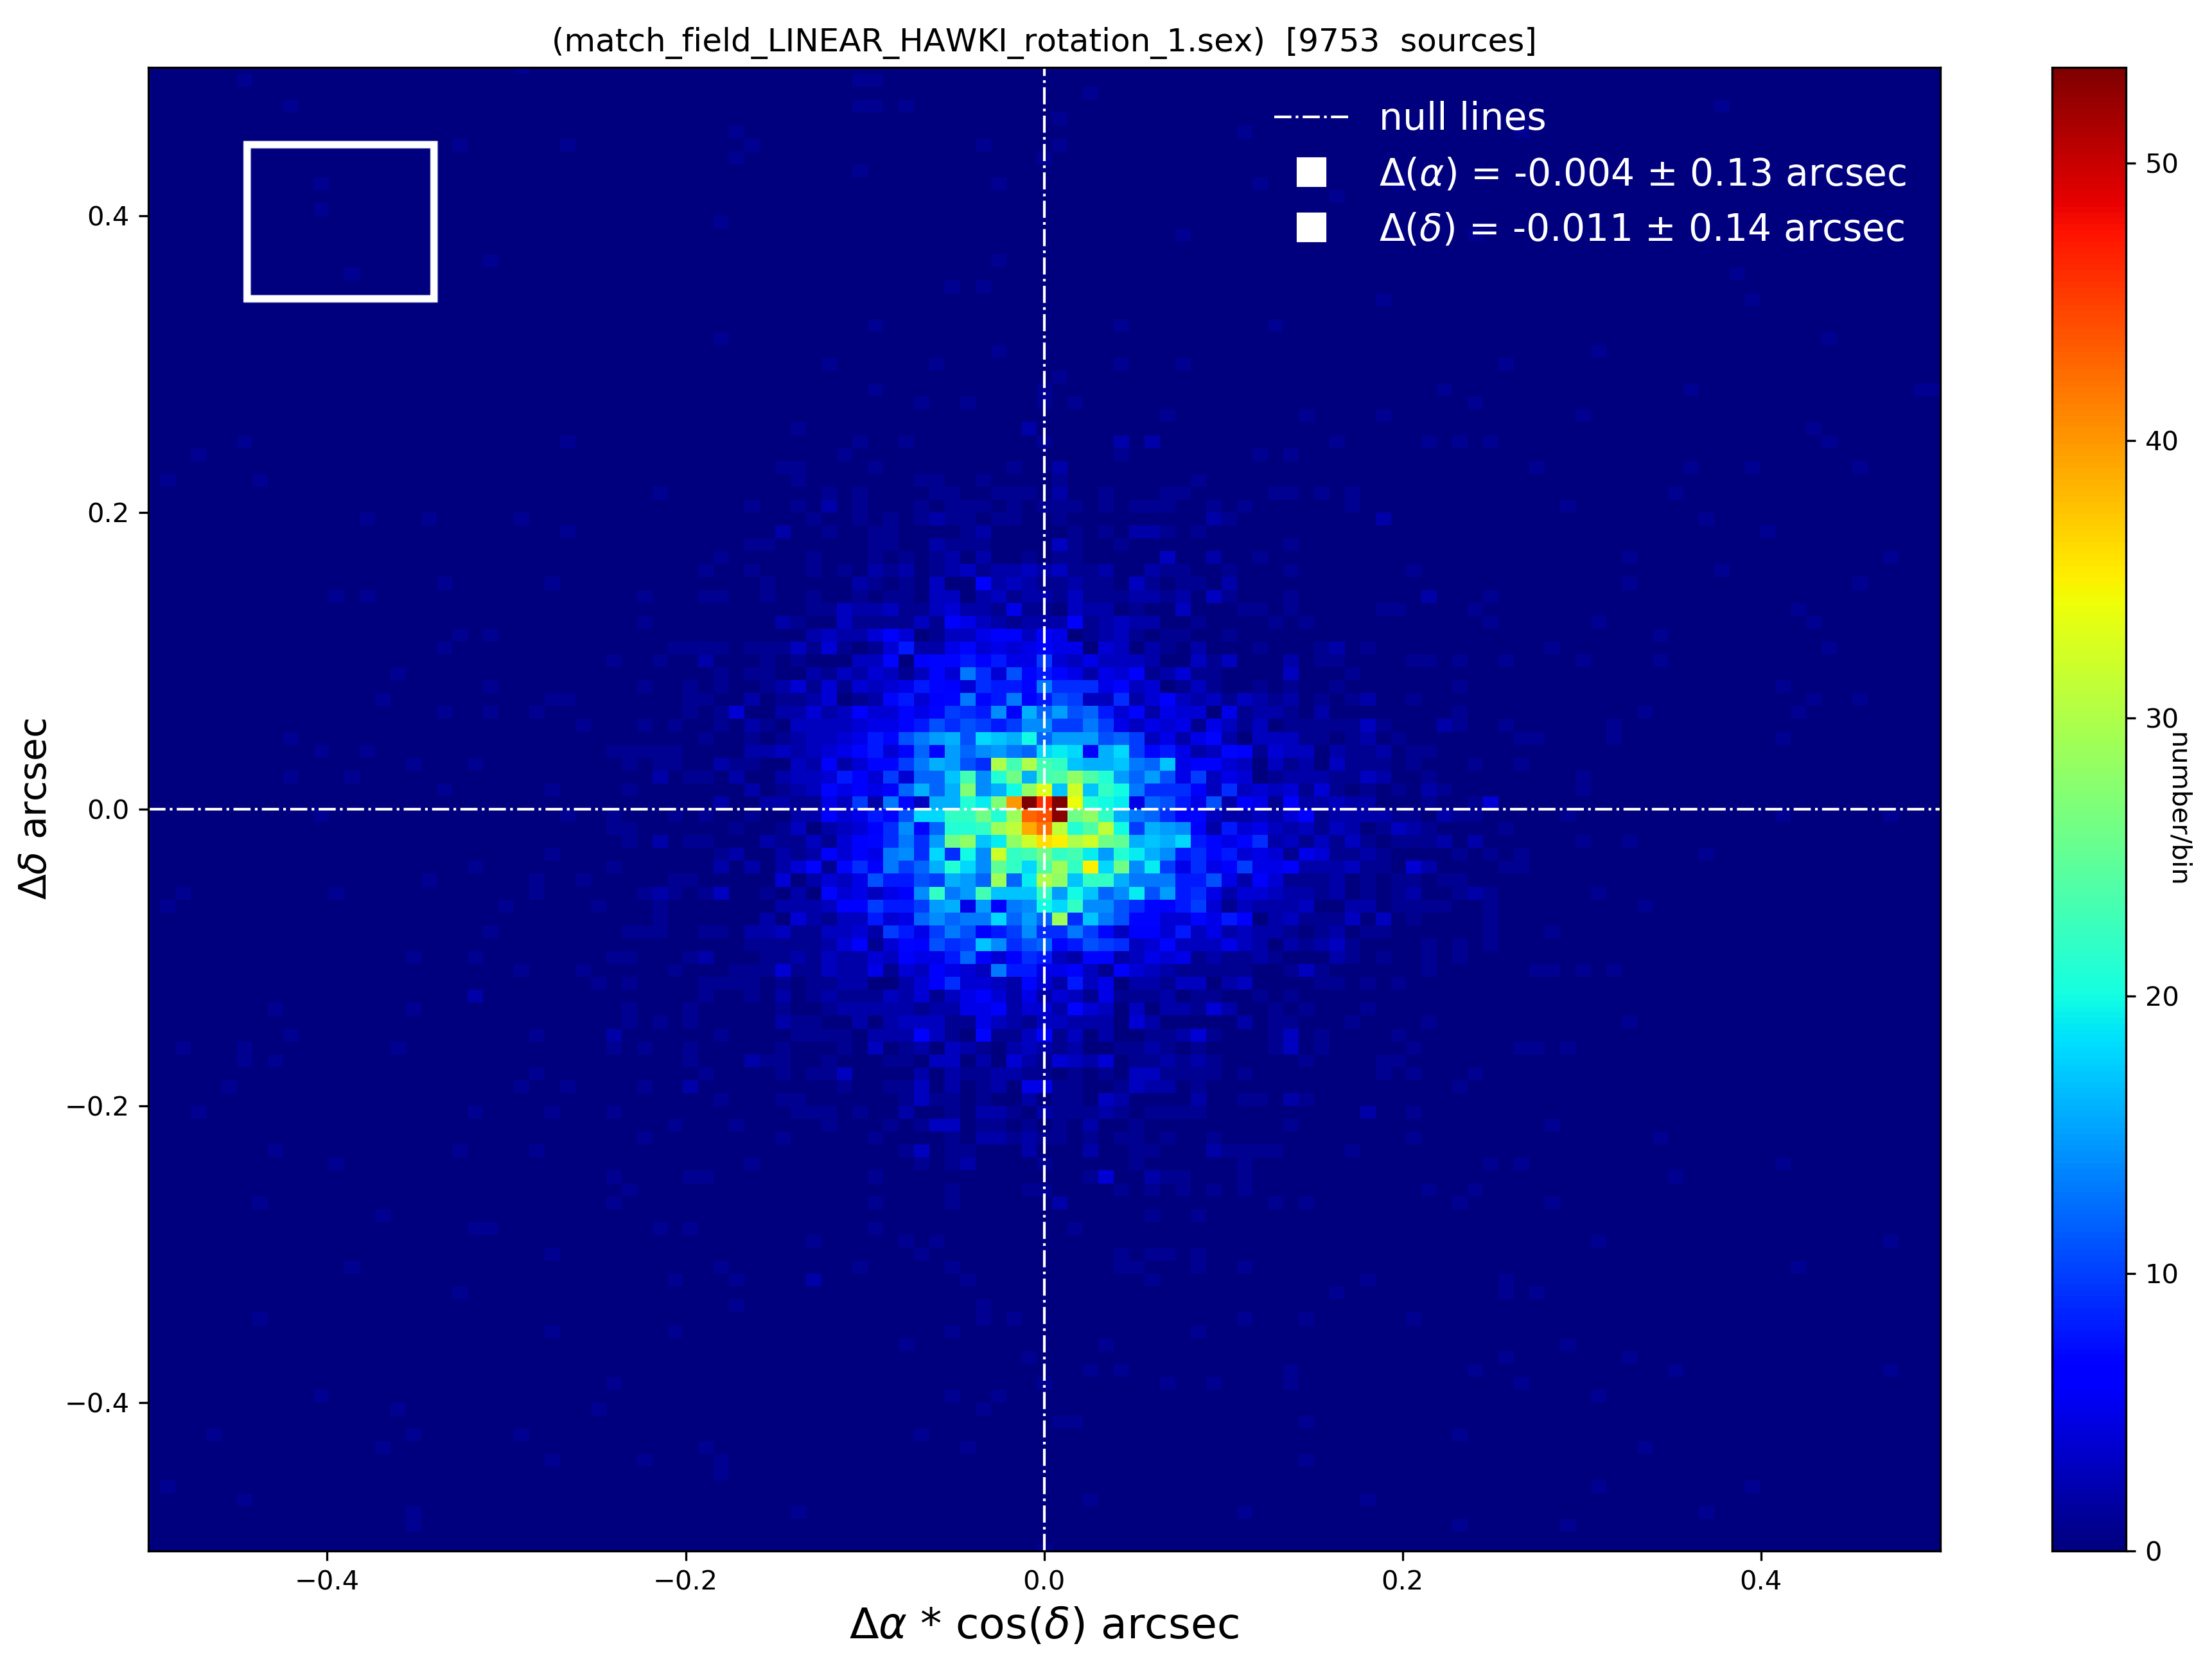
\includegraphics[width=11cm]{figures/match_field_LINEAR_HAWKI_rotation_1_RA_DEC_scatter_plot.png}
\caption[]
	{\footnotesize  the astrometric quality of the \hdrlresample\ routines as measured by comparing 9,753 sources in the original input HAWK-I images
	with those in the resampled ({\tt LINEAR}) image tile of Figure \ref{fig:hawki_flexure}.
	The standard deviation of the $\Delta\alpha*\cos(\delta)$ and $\Delta\delta$ distributions is 0.14 arcsec. This is approximately the size of one HAWK-I
	pixel (0.106 pixels/arcsec).  The pixel size is indicated by the white square in the top left corner.
	}
	\label{fig:radec_flexure}
\end{figure}

Similarly, the photometric quality is also retained following interpolation.   Figure \ref{fig:mag_flexure} is typical of all interpolated frames, with a source magnitude match 
between the individual HAWK-I images and the resampled ({\tt LINEAR}) image tile of $\Delta(mag)=-0.18\pm0.13$ magnitudes.

\begin{figure}[H]
\centering
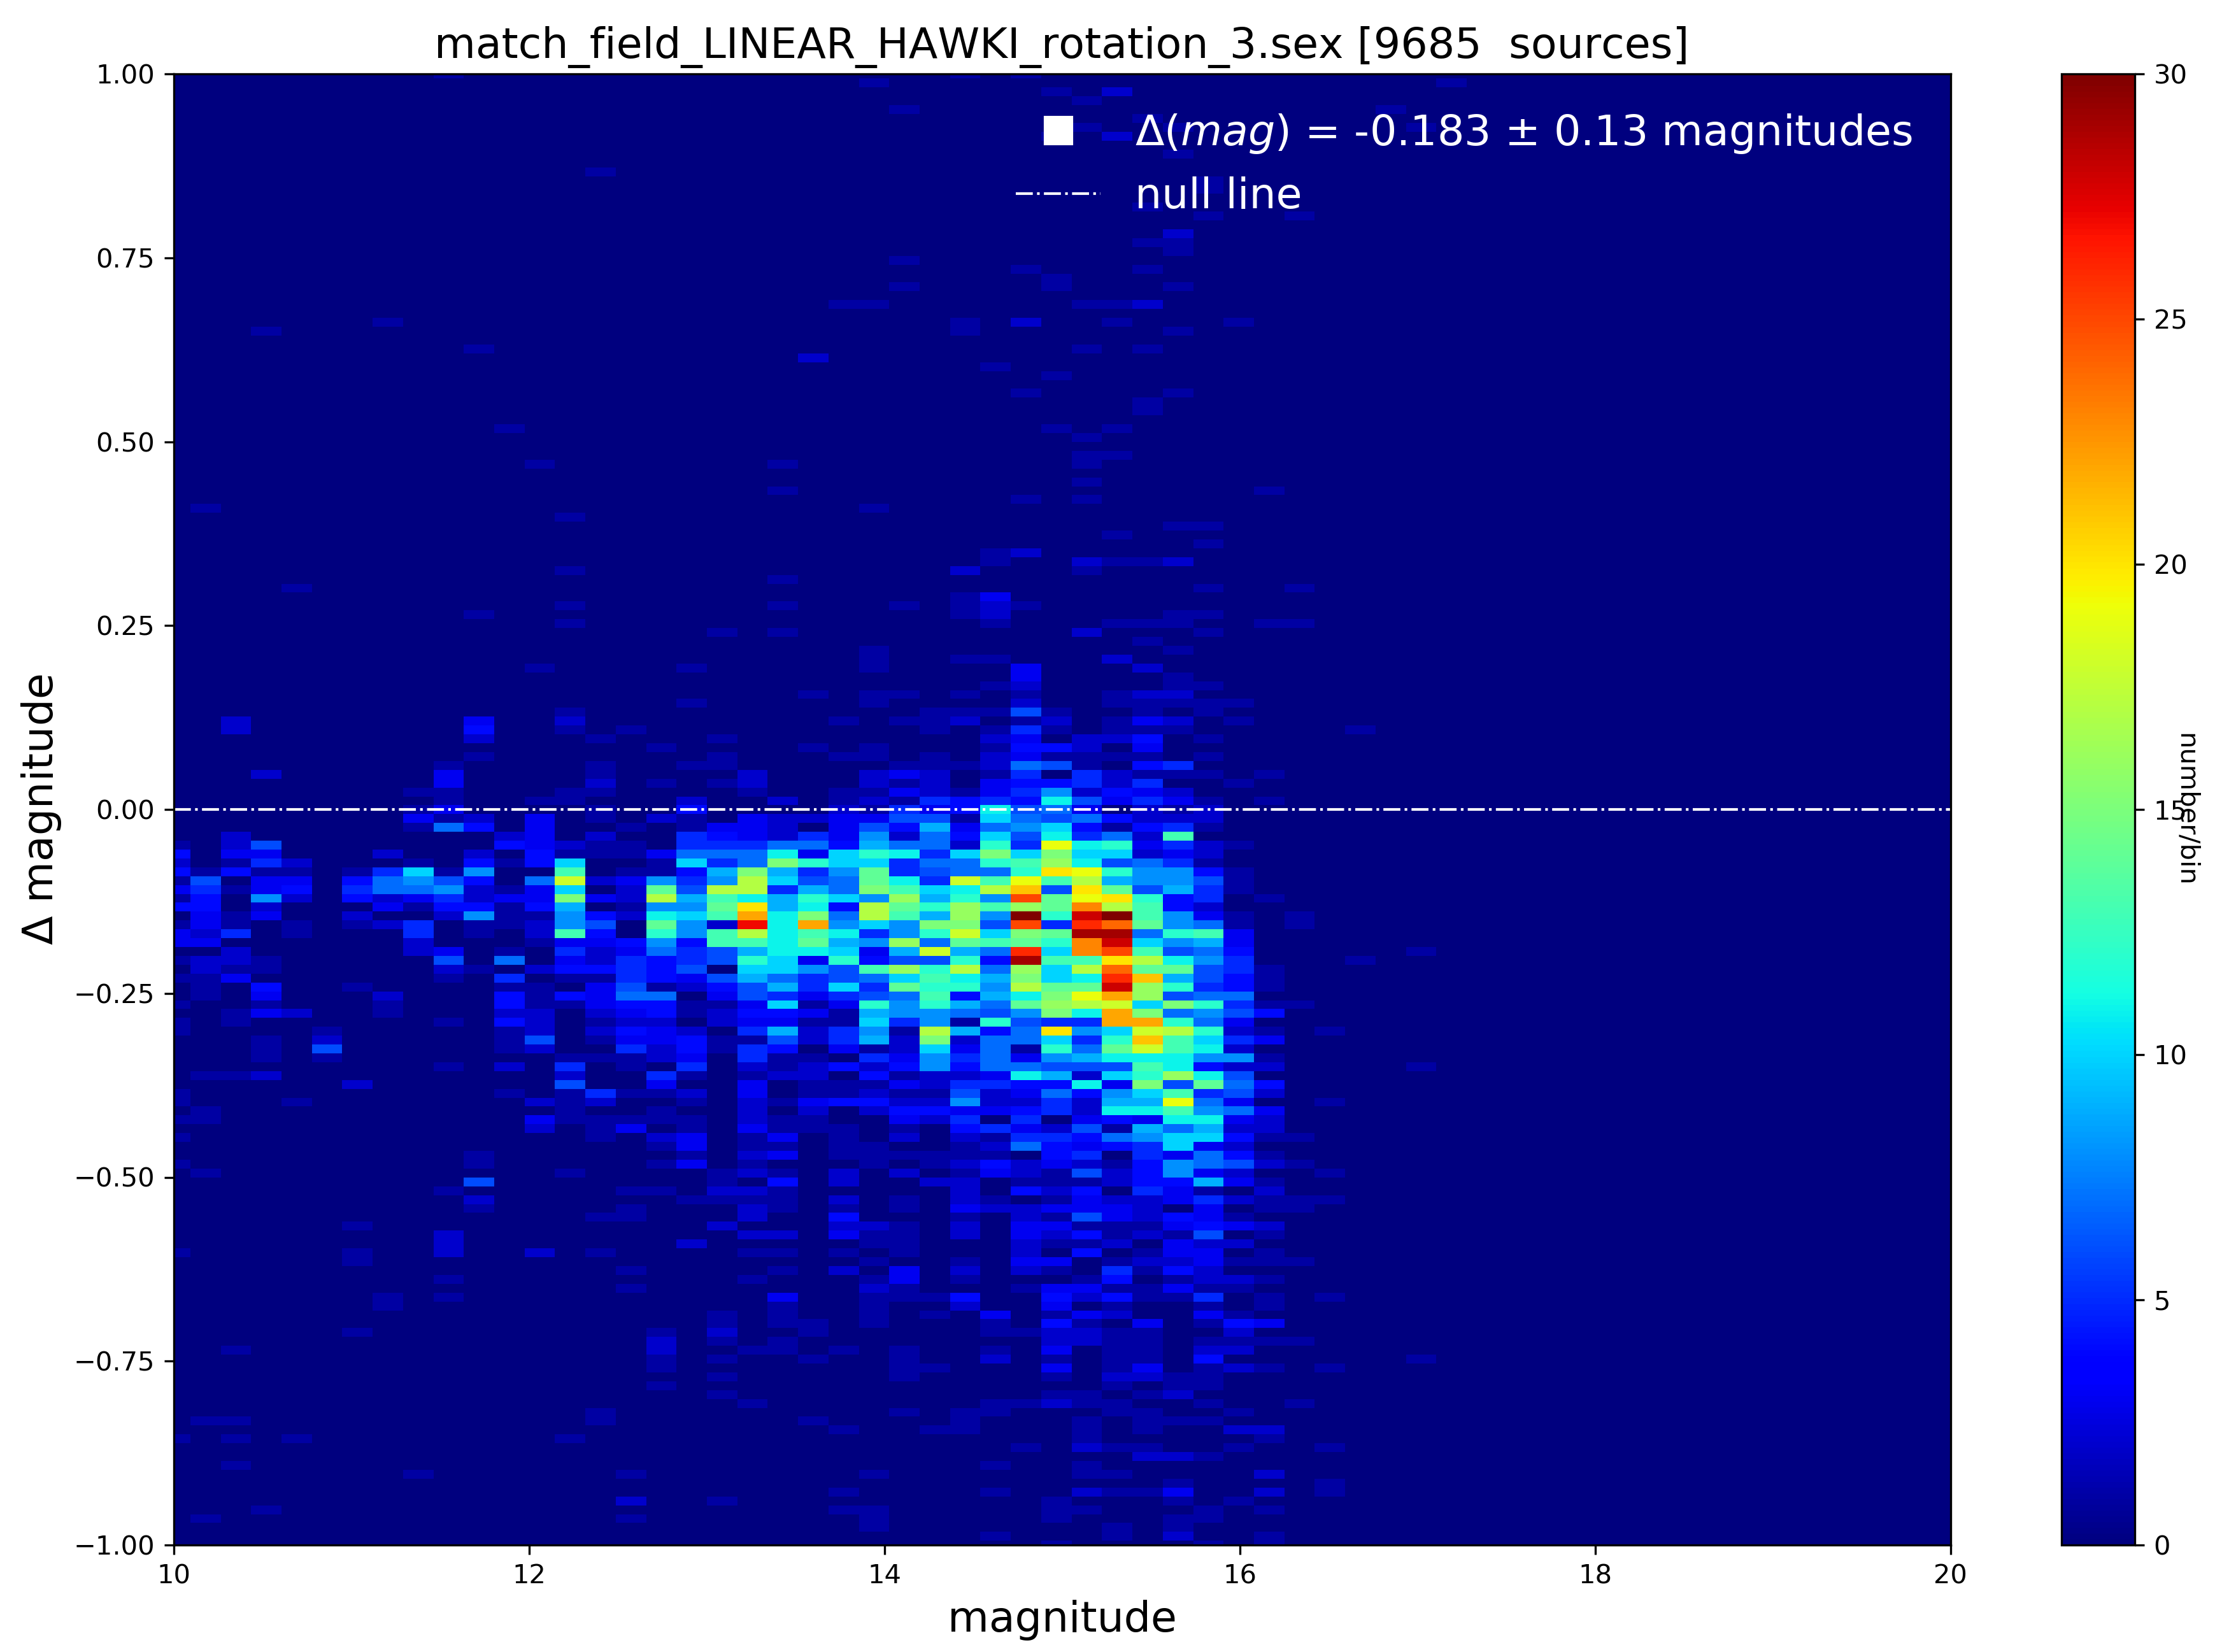
\includegraphics[width=11cm]{figures/match_field_LINEAR_HAWKI_rotation_3_mag_scatter_plot.png}
\caption[]
	{\footnotesize  the photometric quality of the \hdrlresample\ routines as measured by comparing the 9,685 sources in the original input HAWK-I images
	with those in the resampled ({\tt LINEAR}) image tile of Figure \ref{fig:hawki_flexure} (right panel).
	The standard deviation of the $\Delta(mag)$  distribution is 0.13 magnitudes. 	
	}
	\label{fig:mag_flexure}
\end{figure}

As can be seen in figure \ref{fig:fwhm_ellip_flexure}, the resampling causes a slight increase in the FWHM of the sources and a decrease in the source ellipticities.
This is expected, since the resampling will cause a circularisation and homogenisation of the source shapes.


\begin{figure}[H]
\centering
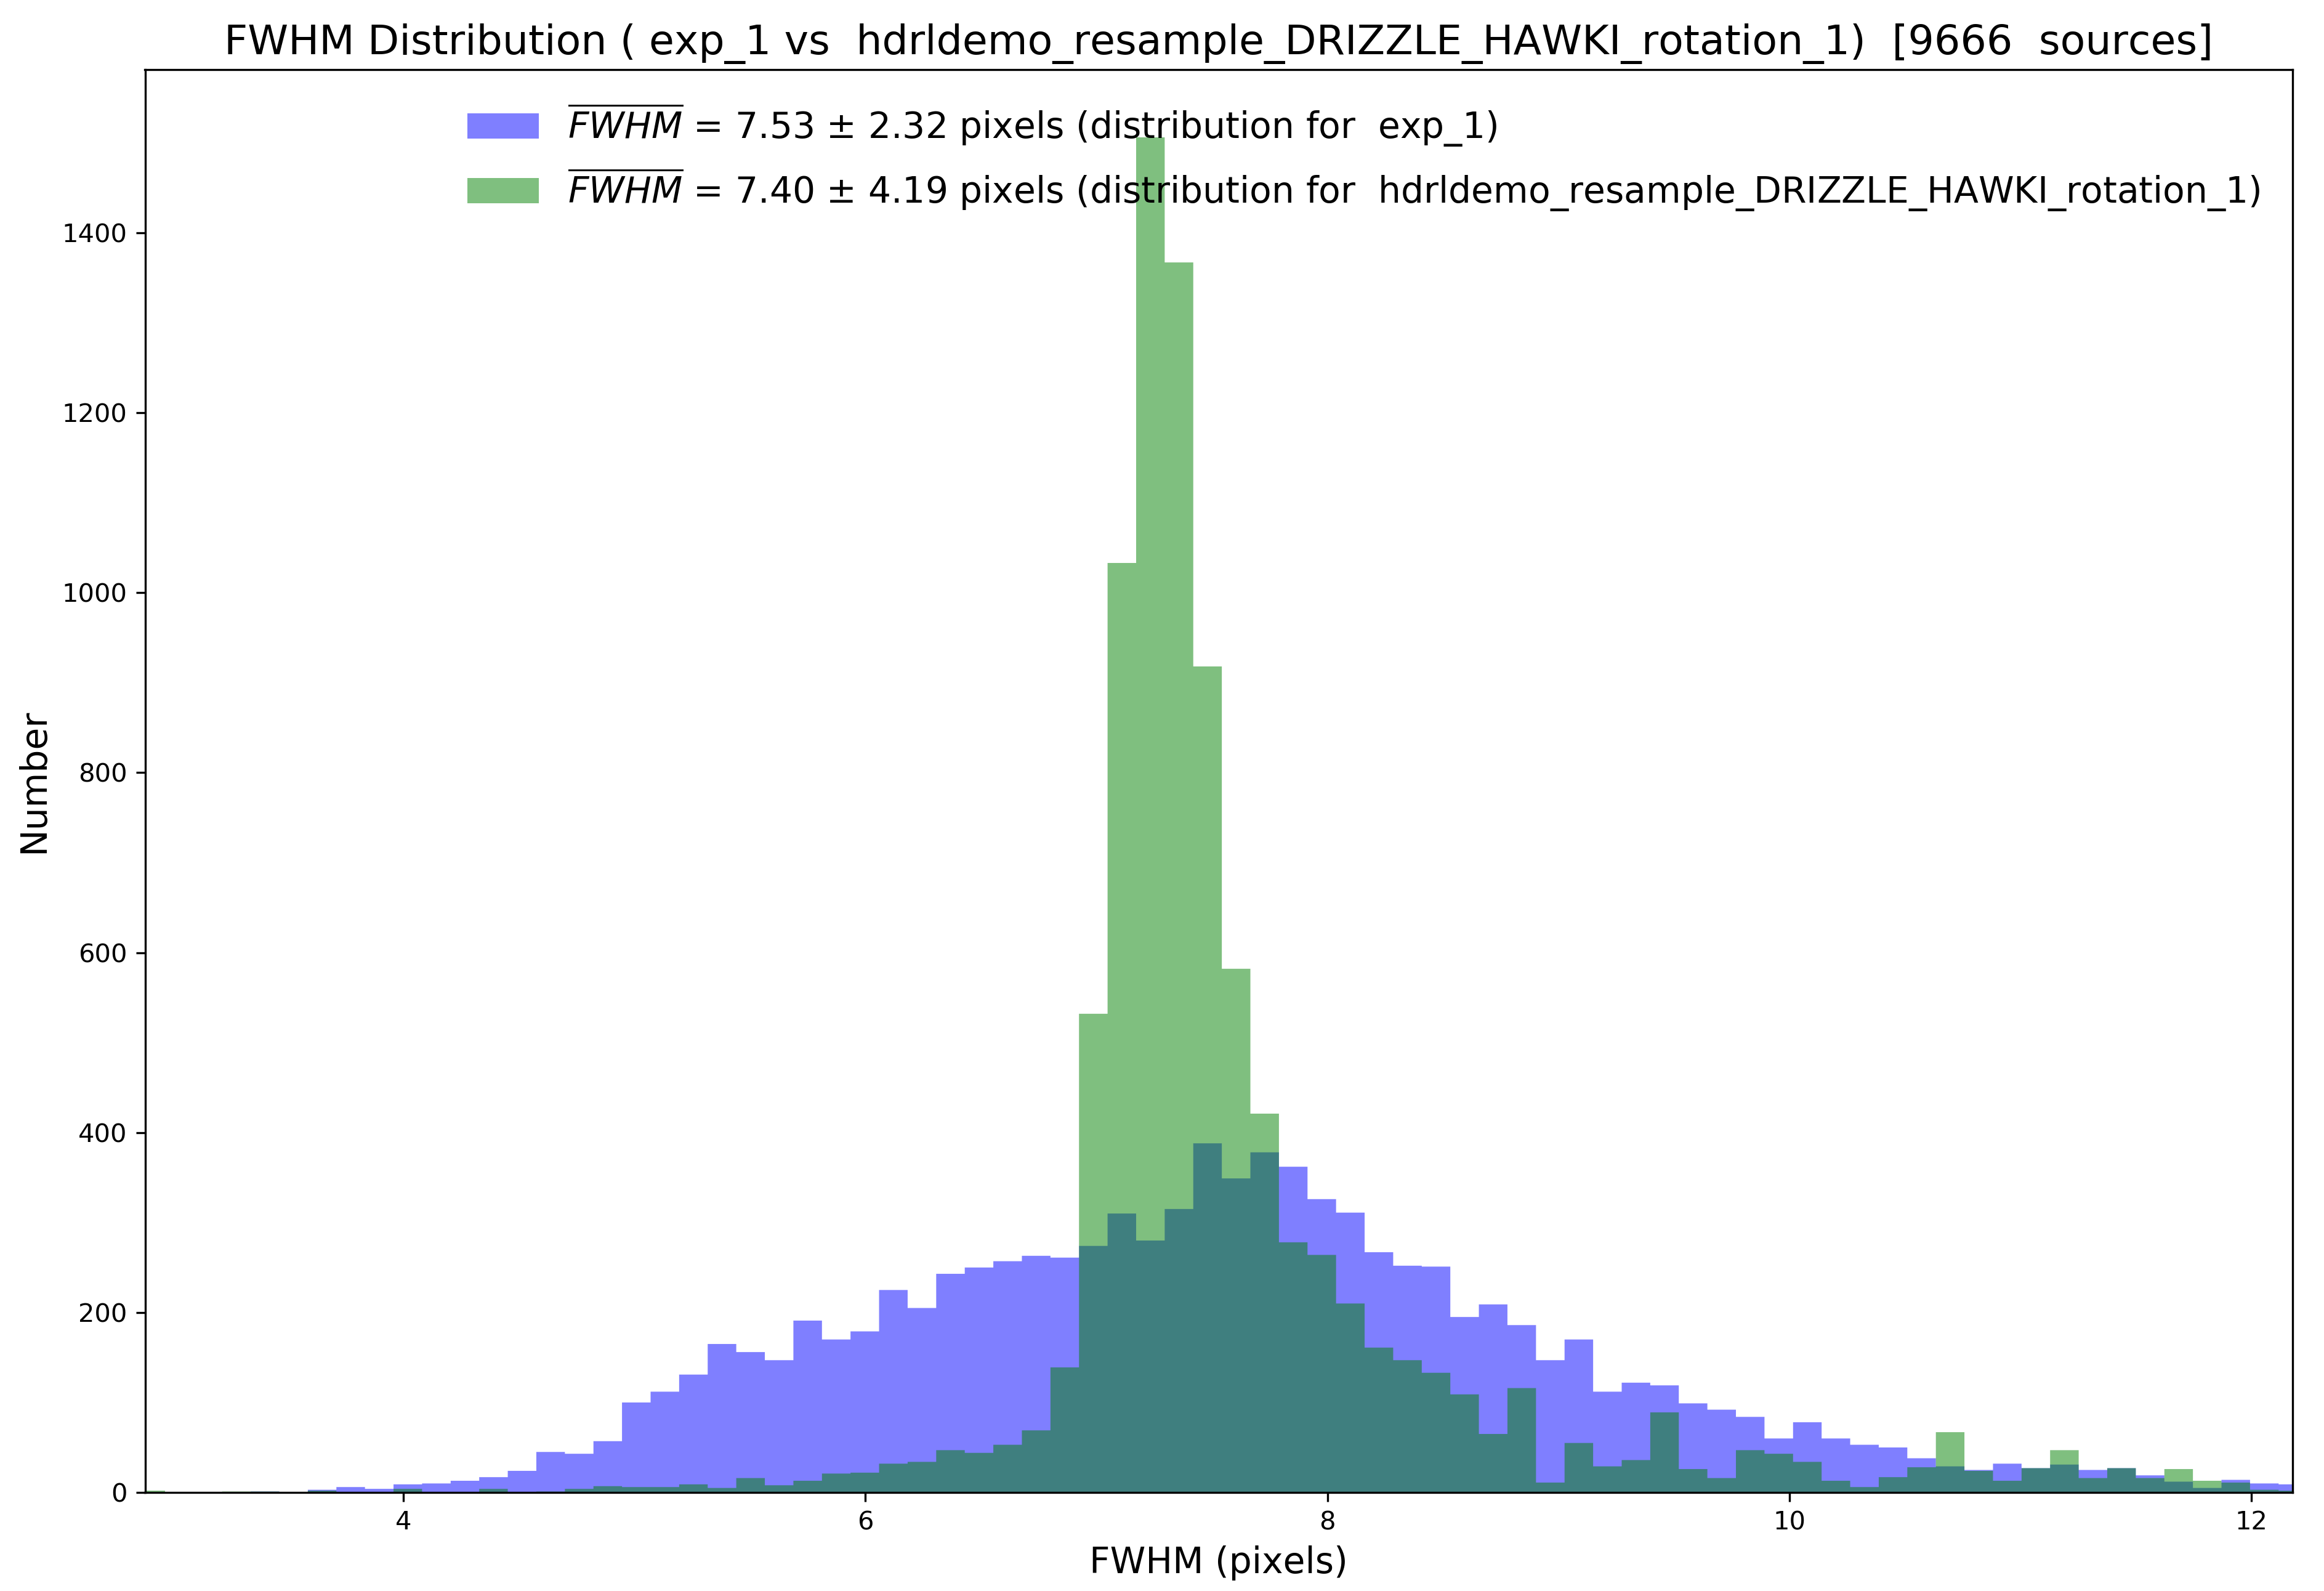
\includegraphics[width=8.4cm]{figures/match_field_DRIZZLE_HAWKI_rotation_1_FWHM_histogram.png}
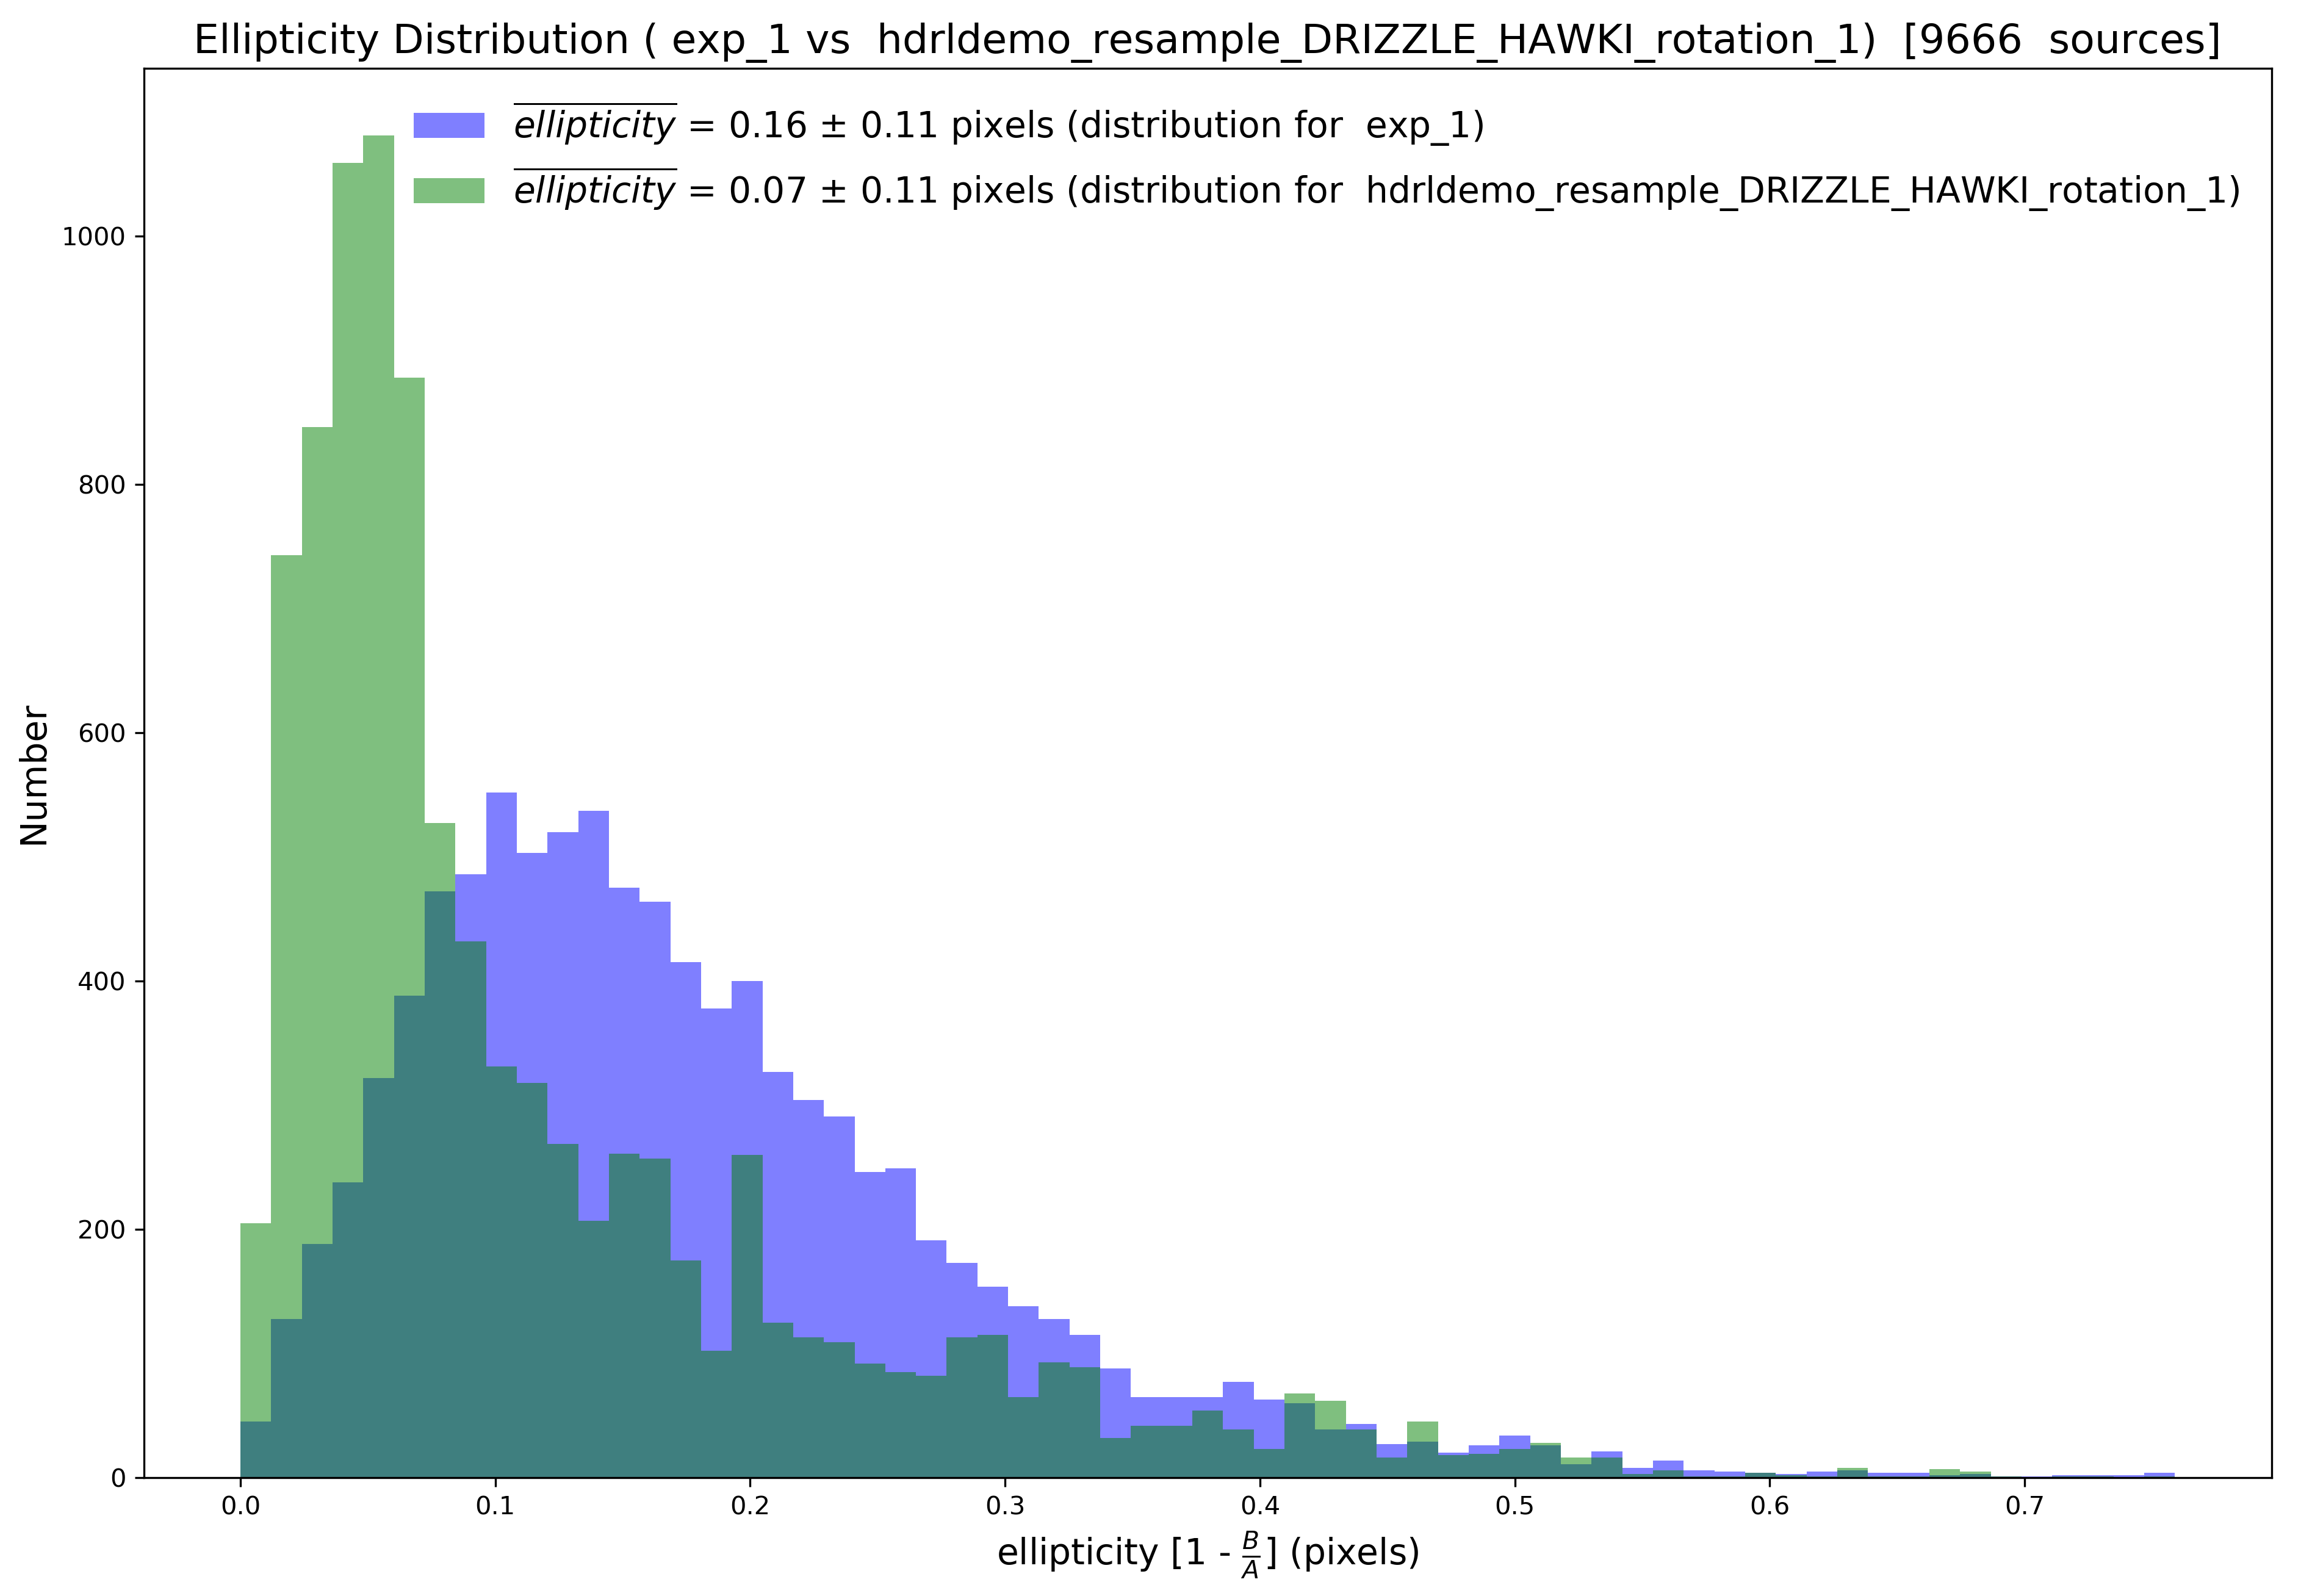
\includegraphics[width=8.4cm]{figures/match_field_DRIZZLE_HAWKI_rotation_1_ellipticity_histogram.png} 
\caption[]
	{\footnotesize  A comparison of FWHM and ellipticity for the sources in the HAWK-I input images (blue histograms) and those
	after resampling (green histograms).  The resampling was done with {\tt --method=DRIZZLE} and {\tt --method.loop-distance=1}.\\
	{\bf left panel:}    The FWHM distribution of the 9,666 sources in the flexure field.  The median FWHM, after resampling, decreases slightly.  
	                           However, this is certainly an artifact of the very broad, ill-defined distribution determined for the input HAWK-I images, being over-estimated.\\
	{\bf right panel:} The distribution of ellipticities.   Here, the resampling has circularised the sources.   This, too, is as expected. 
	}
	\label{fig:fwhm_ellip_flexure}
\end{figure}





A summary of the source attributes between the input frames and the resampled images is given in Table \ref{tab:compare_rotation}.


\begin{sidewaystable}

\caption{A Summary of Comparisons Between Input HAWK-I Flexure Images and Resultant Interpolation Images}

\begin{center}
\begin{tabular}{|l|l|c|c|c|c|c|c|c|c|c|c|}                      
\toprule

Image         				     		     & Interpolation	 & N$_{frames}^2$   & Nmatch & $\Delta\alpha$  & $\Delta\delta$ &  $\Delta(mag)$ & $\sigma\Delta(mag)$ & FWHM1$^3$  & FWHM2$^4$  & ellip1$^3$  & ellip2$^4$  \\
                                     & method (LD)$^1$ &                         &               & (arcsec)            & (arcsec)          &                          &                                   & (pixels)    & (pixels)   &            & \\
\midrule
HAWK-I            & DRIZZLE (1)        & 80    	& 9,666 	& -0.003       & -0.010  	& -0.23 & 0.12          & 7.54  & 7.40  		& 0.16  & 0.07     \\
flexure 	   	& DRIZZLE (3)        & 80    	& 9,666 	& -0.003       & -0.010  	& -0.23 & 0.12 	  	& 7.54  & 7.40  		& 0.16  & 0.07  \\
 	               	& LANCZOS (1)      & 80    	& 9,675 	& -0.003       & -0.009  	& -0.23 & 0.12          & 7.54  & 7.36  		& 0.16  & 0.07   \\
 	   	      	& LANCZOS (3)      & 80    	& 9,657 	& -0.003       & -0.009  	& -0.23 & 0.12          & 7.54  & 7.30  		& 0.16  & 0.07     \\
 	              	& LINEAR (1)          & 80      	& 9,753 	& -0.004       & -0.011  	& -0.21 & 0.12          & 7.54  & 7.61  		& 0.16  & 0.09     \\
 	              	& LINEAR (3)          & 80      	& 9,685 	& -0.004       & -0.013  	& -0.18 & 0.13          & 7.54  & 8.66  		& 0.16  & 0.11     \\
 	              	& NEAREST (1)      & 80     	& 7,788 	& -0.001       & 0.004  	& -0.26 & 0.13          & 7.54  & 7.79  		& 0.16  & 0.14     \\
 	              	& NEAREST (3)      & 80     	& 7,788 	& -0.001       & 0.004  	& -0.26 & 0.13          & 7.54  & 7.79  		& 0.16  & 0.14     \\
 	              	& QUADRATIC (1)  & 80   	& 9,444 	& -0.003       & -0.008  	& -0.22 & 0.13         & 7.54  & 7.75  		& 0.16  & 0.08     \\
 	              	& QUADRATIC (3)  & 80   	& 9,470 	& -0.004       & -0.010  	& -0.21 & 0.13          & 7.54  & 8.00   		& 0.16  & 0.08     \\
 	              	& RENKA (1)           & 80   	& 9,387 	& -0.004       & -0.007  	& -0.24 & 0.12         & 7.54  & 7.72 		& 0.16  & 0.08     \\
                		& RENKA (3)           & 80    	& 9,387 	& -0.004       & -0.007  	& -0.24 & 0.12          & 7.54  & 7.72  		& 0.16  & 0.08     \\
\bottomrule


\end{tabular}	
\end{center}																											

\label{tab:compare_rotation}
\noindent{
		$^1$ The interpolation method and loop-distance used ({\tt --method.loop-distance}).\\
		$^2$ The total number of single, HAWK-I input images combined during the resampling.\\
		$^3$ FWHM1 and ellip1 refer to the original, HAWK-I input images.\\
		$^4$ FWHM2 and ellip2 refer to the resampled images.}
\end{sidewaystable}



\subsection{The Propagation of Edge Effects with Resampled Images}

Astronomical detectors often have edge effects in which the outermost regions of the detector show strongly depressed flux levels.
This can be due to a non-uniform illumination over the surface of the detector, or due to masked edges.   This is particularly evident
in some near infrared detectors.

An edge effect will be strongly enhanced by any resampling method as the algorithm interpolates across such an illumination
discontinuity.   This can be seen in figure \ref{fig:hawki_edges}.  Here, the images of M30 were resampled without first trimming their
edges.  This image should be compared to the right hand panel of figure \ref{fig:hawki_M30}.

The \hdrlresample\ suite will need to include a parameter that allows for the input images to be edge trimmed before
being resampled and combined.  The parameter should be defined as {\tt --edge-trim=NN}, whereby {\tt NN} sets the number of pixels
trimmed from each of the four sides of each input image.
This parameter has already been implemented in the HDRL pipeline kits from version 15 ({\it hdrldemo-kit-1.3.0-15}).

\begin{figure}[H]
\centering
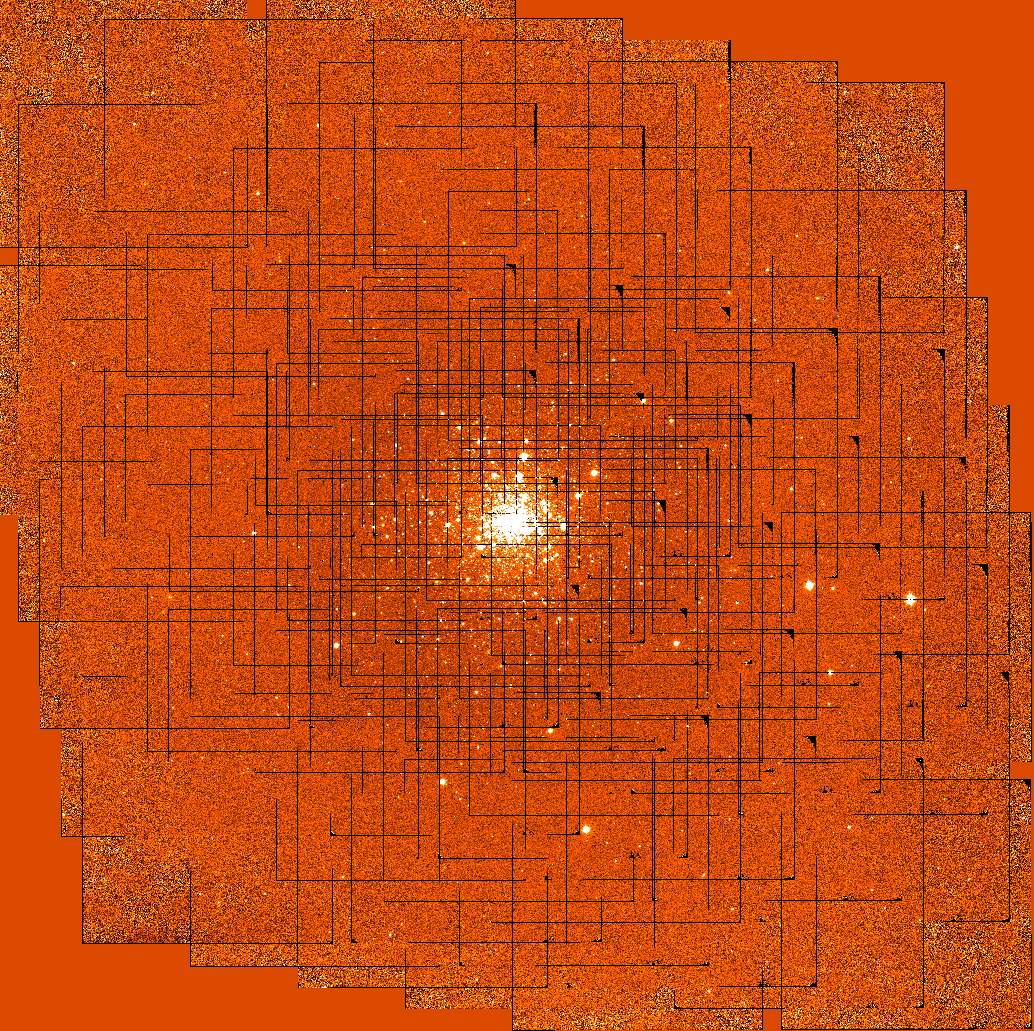
\includegraphics[width=8.4cm]{figures/hdrldemo_resample_DRIZZLE_HAWKI_M30_3.png}
\caption[]
	{\footnotesize  An example of strong edge effects in the final tile image made from 100 HAWK-I images of the M30 field.
	This image has been resampled and combined using \hdrlresample\ with {\tt --method=DRIZZLE} and {\tt --method.loop-distance=1}, 
	without trimming the discontinuities at the edge of each input HAWK-I image.\\
	}
	\label{fig:hawki_edges}
\end{figure}




\subsection{Results from Synthetic Images With Right Ascension values At the Meridian and Declination near the Poles}

A potential pitfall can occur when images straddle discontinuities in the WCS coordinate system.  Therefore, a series of 10 dithered synthetic images were created
with a central pixel values set to reference points:\\
({\tt CRVAL1, CRVAL2}) = $(\alpha_{\circ}, \delta_{\circ})$ = (360$^\circ$, 88$^\circ$). \\
These synthetic images were then resampled and combined using the six available \hdrlresample\ methods.   In each case, the resampled frames correctly retain the
celestial coordinates of the original input images.   This can seen in figure \ref{fig:discontinuity}, in which the ds9 coordinate grid is overlaid on the images and displays
the correct transition straddling the $0^\circ$ meridian.


\begin{figure}[H]
\centering
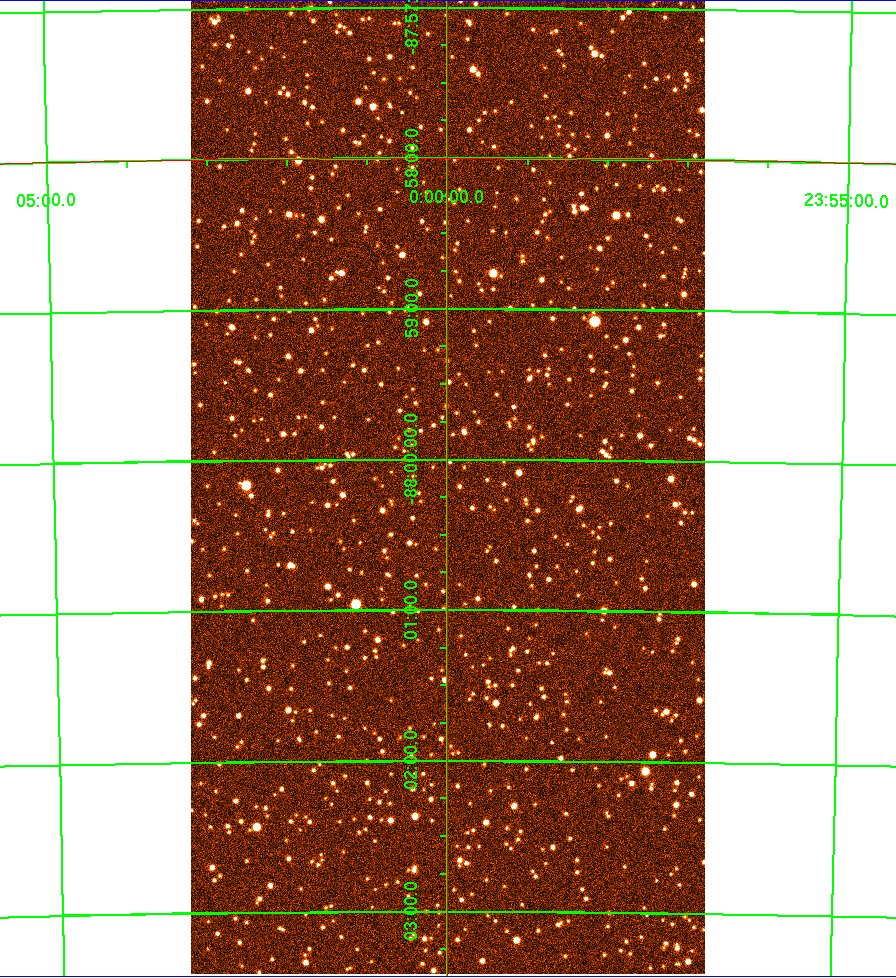
\includegraphics[width=8.1cm]{figures/synth_disc2_stars_gal_bkgd_1.png}
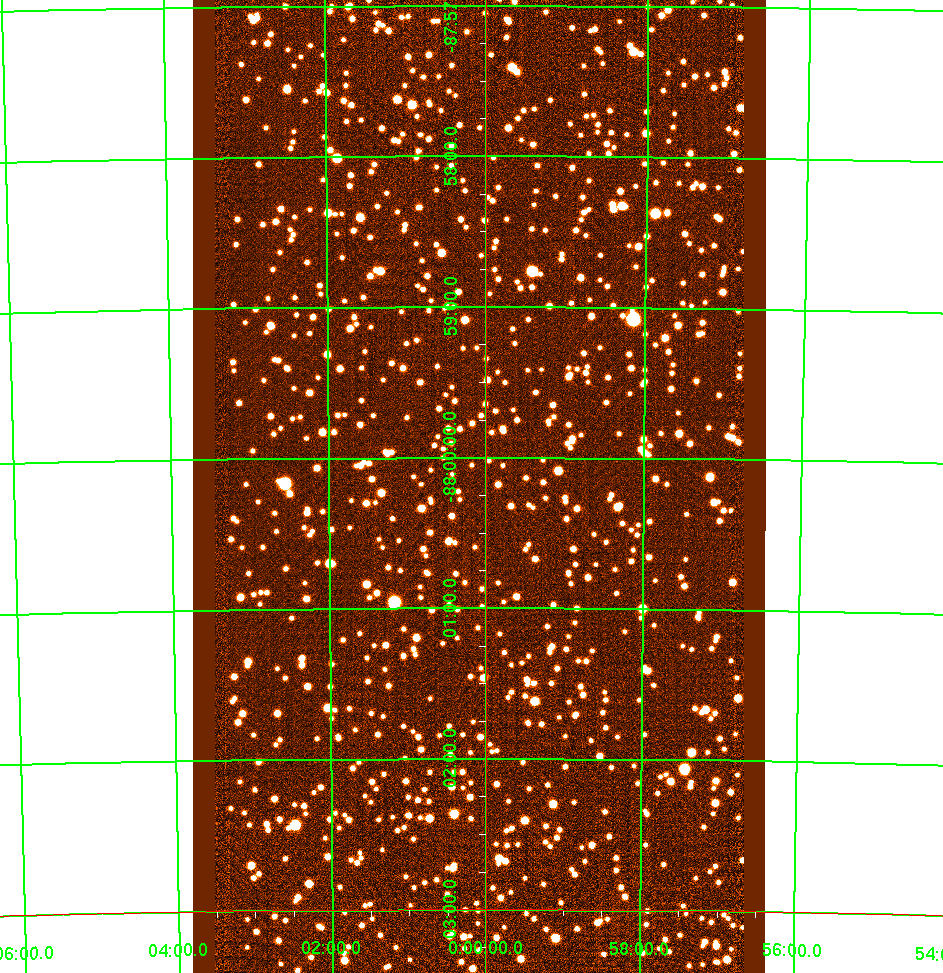
\includegraphics[width=8.6cm]{figures/hdrldemo_resample_DRIZZLE_disc2_coadd_1.png} 
\caption[]
	{\footnotesize  A synthetic image and its resampled counterpart to test the \hdrlresample\ routines at and near celestial discontinuities  \\
	{\bf left panel:}    A single synthetic frame with {\tt (CRVAL1, CRVAL2)} =  $(\alpha, \delta) = 360^\circ, -88^\circ$).      \\
	{\bf right panel:}  The ten synthetic resampled and combined using \hdrlresample\ with {\tt --method=DRIZZLE} and {\tt --method.loop-distance=1}.\\
	The overlaid ds9 coordinate grid shows that these extreme $(\alpha, \delta)$ values are handled correctly.
	}
	\label{fig:discontinuity}
\end{figure}



\subsection{Testing the \hdrlresample\ Routines Using MUSE Data Cubes}

Tests on MUSE datacubes were performed on dithered observations of two
targets: TNJ2009-304 (a protocluster at z$\sim$3) and FCC 184 (an
early-type galaxy in the Fornax cluster).

The cube of TNJ2009-304 includes the combination of 6 dithered
exposures (MUSE.2016-06-01T06:09:25.499.fits,
MUSE.2016-06-01T07:05:35.072.fits, MUSE.2016-06-01T08:24:39.641.fits,
MUSE.2016-06-01T09:19:35.838.fits, MUSE.2016-06-08T06:06:02.858.fits,
and MUSE.2016-06-08T06:58:50.486.fits).

 The cube of GCC 184 includes
the combination of 10 dithered exposures
(MUSE.2017-01-26T02:57:56.013.fits, MUSE.2017-01-26T03:16:12.338.fits,
MUSE.2017-01-26T03:30:08.819.fits, MUSE.2017-01-26T03:49:23.358.fits,
MUSE.2017-01-26T04:03:20.921.fits, MUSE.2017-11-15T06:57:38.494.fits,
MUSE.2017-11-15T07:15:56.735.fits, MUSE.2017-11-15T07:29:49.482.fits,
MUSE.2017-11-15T07:48:08.059.fits, and
MUSE.2017-11-15T08:02:02.941.fits).


First, the data were reduced and combined with the MUSE pipeline
(v2.8.3). This process foresees the combination of so-called
pixel-tables, each of them represent the fully reduced exposure in
detector space. The direct combination of pixel tables implies one
single regridding process of the data.


The MUSE pipeline also produced the regridded cubes of the individual
exposures, which we then combined (after taking into account spatial
offsets in RA/DEC) with the HDRL recipe \hdrlresample. This process
implies two regriddings: the first is done by the MUSE pipeline to
``convert'' each pixel table into a datacube. The second is done by
HDRL to regrid each cube into a common WCS before combining them.

The combination was done using the same parameters as in MUSE; drizzle
method with downscaling factor 0.6 (spatial and spectral dimension),
and loop-distance =1 pixel. The variance extension in the MUSE
individual datacubes was also used.

Also, we set the starting and ending RA/DEC in the HDRL recipe so that
the final cube spatially matches the MUSE combined cube.  In this way a
direct 1-to-1 spaxel comparison is possible.

The goals are to compare the quality of the spatial resolution and
spectra obtained with two approaches; a direct combination of reduced
pixel-tables with the MUSE pipeline, and the combination of individual
pre-regridded cubes with HDRL.


\subsubsection{Spatial resolution}

Figure \ref{fig:muse_hdrl_fov} compares the white-lamp images obtained
by collapsing the MUSE and HDRL datacubes along the wavelength
axis. The HDRL cubes are smoother in the spatial direction, as a
consequence of the two-regridding steps that are involved in the
process. Table \ref{tab:compare_psf_muse} compares the MOFFAT point
spread function (measured with IRAF) of point-like sources measured on
the reconstructed images. On average, the HDRL cubes have FWHM 1-2\%
higher than the corresponding source in the MUSE cube.

 
\begin{table}
\caption{Point spread function of point-like sources in the reconstructed field of views}
\begin{center}
\begin{tabular}{l c c c c c c}
 ID &  X   &     Y  &     RA    &  DEC        &   MOFFAT\_MUSE& MOFFAT\_HDRL \\
    &  pxl &   pxl  & [$^\circ$] &  [$^\circ$]  &   pxl   &    pxl \\
\hline
    &      &        &           &  TNJ2009-304  &         &         \\
1   &40.48 & 285.49 &302.4580383 &--30.6613064 &  4.73   &  4.75   \\ 
2   &97.99 & 190.29 &302.4543457 &--30.6665955 &  4.49   &  4.56   \\
3   &168.09&  214.34& 302.4497986& --30.6652584&   4.53  &   4.61  \\
4   &262.61&  215.91& 302.4436951& --30.6651707&   5.78  &   5.85  \\
5   &254.20&  189.76& 302.4442444& --30.6666241&   4.30  &   4.41  \\
6   &155.89&  143.03& 302.4505920& --30.6692200&   4.78  &   4.82  \\
    &      &        &            &   FCC184    &         &         \\
7   &194.40&  355.39&  54.2386971& --35.4991646&   4.50  &    4.59 \\ 
\hline
\end{tabular}	
\end{center}																				
\label{tab:compare_psf_muse}
\end{table}




\begin{figure}[H]
\centering
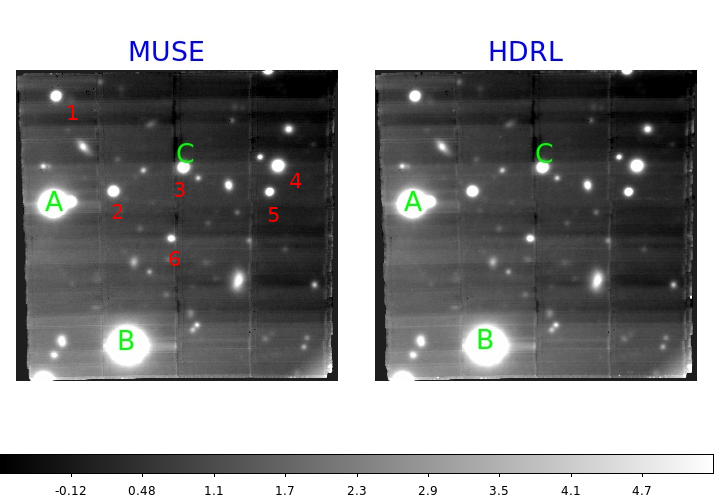
\includegraphics[width=17cm]{figures/fovs.jpg}
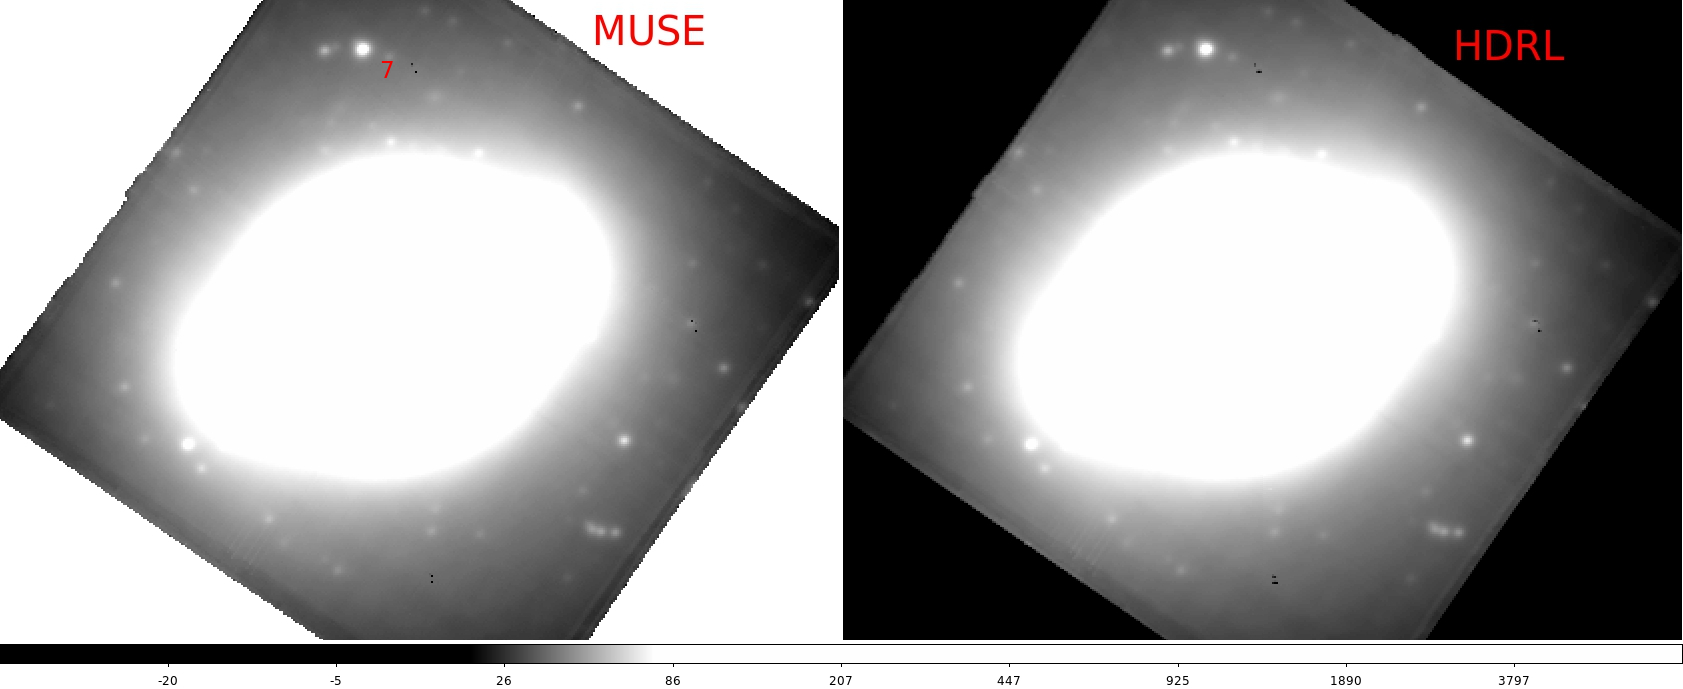
\includegraphics[width=17cm]{figures/fovs2.jpg}
\caption[] {\footnotesize Comparison between the reconstructed fields
  of view obtained by combining individual reduced pixel tables with
  the MUSE pipeline (left) and by combining individual reduced cubes
  with hdrl\_demo\_resample (right). The figure on the top refers to
  TNJ2009-304, the figure on the bottom to FCC 184. The numbers
  indicate the sources we measured the Moffat PSF in Table
  \ref{tab:compare_psf_muse}. The letters indicate the sources we
  compare in the spectra of figures \ref{fig:muse_hdrl_spaxel} to
  \ref{fig:muse_hdrl_profile}. }
	\label{fig:muse_hdrl_fov}
\end{figure}


\subsubsection{Difference in spectra}

In this section we quantify the differences in the spectral properties
due to the different resampling scheme. The analysis is done for the 3
sources in the field of TNJ2009-304, marked as A, B, and C in Figure
\ref{fig:muse_hdrl_fov}.

The first effect of the smearing in the spatial resolution is that in
the HDRL cube the flux is distributed on a larger area than in the
MUSE cube. Therefore, at each spaxel the flux level is different; in
the studied sources this difference can be as large as 5\% (see figure
\ref{fig:muse_hdrl_spaxel}), but it obviously depends on the spatial
profile, the difference being larger for more peaked profiles.

We then measured the changes in the integrated flux of individual
sources; we compared the flux of some sources integrated on a 5x5 box
around the source peak.  This comparison is shown in figures
\ref{fig:muse_hdrl_spcA}--\ref{fig:muse_hdrl_spcC}.

As shown in these figures, there are small difference between spectra
of the same source extracted from the MUSE and HDRL datacubes, of the
order of 1-2\%. The S/N ratio of the spectra extracted from the cube
produced by HDRL is a few percent higher than the S/N of spectra
extracted from datacubes combined with the MUSE pipeline; this is
expected, as the two regridding process also smooths the spectra along
the wavelength direction.

Figure \ref{fig:muse_hdrl_profile} shows the comparison between the
spectra of source A on a wavelength region around prominent absorption
lines (CaT). The figure shows that, while the continuum of the two
spectra is more or less the same (a small offset $<0.5$\% is visible),
the shape of the absorption lines differ by $\approx 1$\%. This means
that the combination of datacubes (that implies 2 resamplings) can
``damage'' the shape of line features by $\approx $1\% with respect to
the combination of reduced pixel tables.




\begin{figure}[H]
\centering
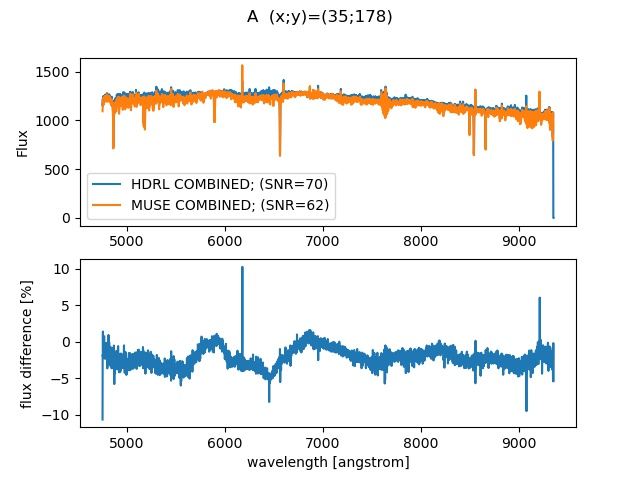
\includegraphics[width=12cm]{figures/spc_A_single_spaxel.jpg}
\caption[] {\footnotesize Top panel. Comparison between the central spaxel
  of source A shown in \ref{fig:muse_hdrl_fov} in the cube obtained by
  combining individual reduced pixel tables with the MUSE pipeline
  (left orange) and the one obtained by combining individual reduced
  cubes with hdrl\_demo\_resample (blue). Bottom panel, the difference
  in percentage between the 2 spectra of the top panel. }
	\label{fig:muse_hdrl_spaxel}
\end{figure}


\begin{figure}[H]
\centering
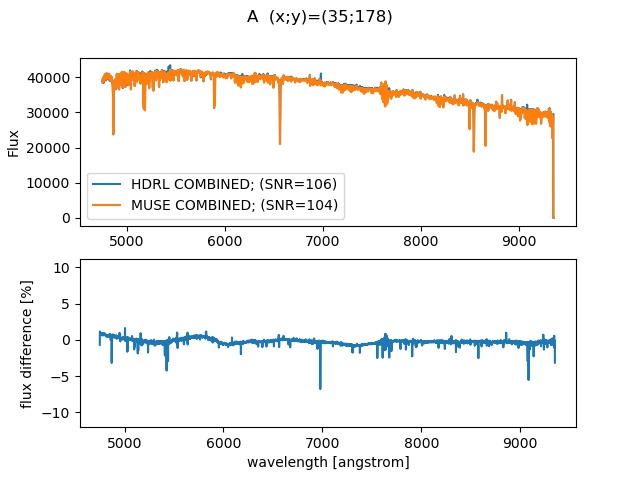
\includegraphics[width=12cm]{figures/spc_A.jpg}
\caption[] {\footnotesize Top panel. Comparison between the spectrum
  of source A shown in \ref{fig:muse_hdrl_fov} in the cube obtained by
  combining individual reduced pixel tables with the MUSE pipeline
  (left orange) and the one obtained by combining individual reduced
  cubes with hdrl\_demo\_resample (blue). The spectrum is obtained by
  integrating a 7x7 box around the spaxel indicated in the
  image. Bottom panel, the difference in percentage between the 2
  spectra of the top panel.}
	\label{fig:muse_hdrl_spcA}
\end{figure}


\begin{figure}[H]
\centering
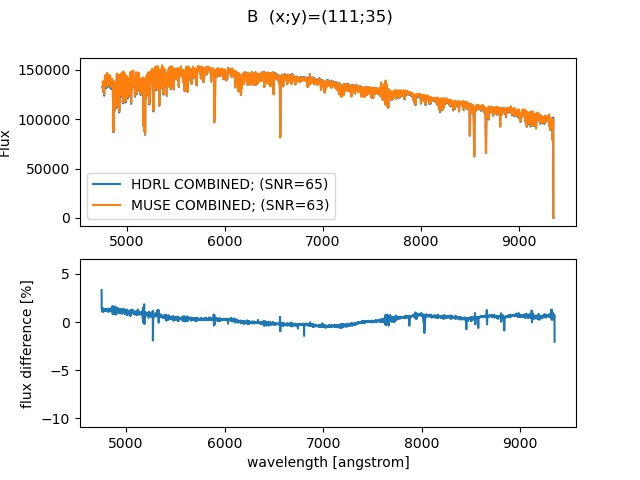
\includegraphics[width=12cm]{figures/spc_B.jpg}
\caption[] {\footnotesize As in figure \ref{fig:muse_hdrl_spcA}, but for source B in figure \ref{fig:muse_hdrl_fov}.}
	\label{fig:muse_hdrl_spcB}
\end{figure}

\begin{figure}[H]
\centering
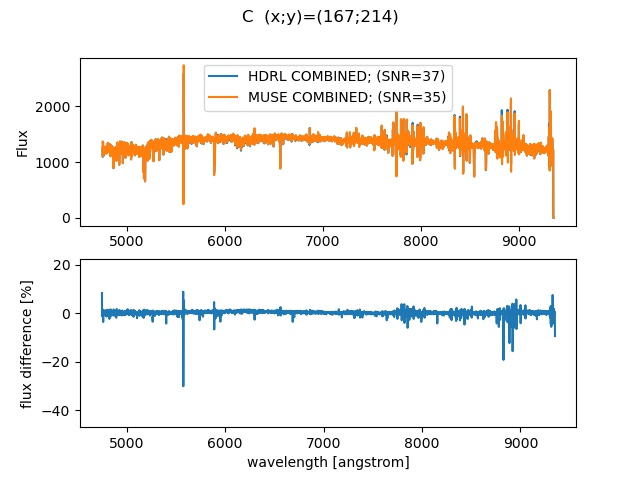
\includegraphics[width=12cm]{figures/spc_C.jpg}
\caption[] {\footnotesize As in figure \ref{fig:muse_hdrl_spcA}, but for source C in figure \ref{fig:muse_hdrl_fov}.}
	\label{fig:muse_hdrl_spcC}
\end{figure}

\begin{figure}[H]
\centering
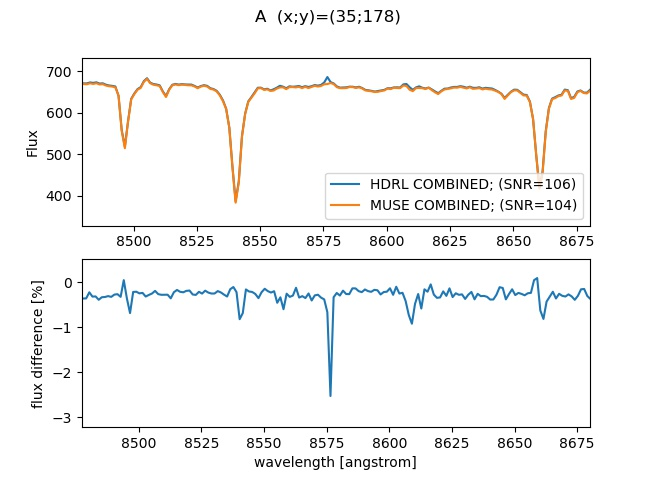
\includegraphics[width=12cm]{figures/line_shape.jpg}
\caption[] {\footnotesize As in figure \ref{fig:muse_hdrl_spcA}, but for the wavelength region around CaT absorption features.}
	\label{fig:muse_hdrl_profile}
\end{figure}


\subsubsection{Difference in derived properties}

In this section we measure the differences in physical properties
derived from the analysis of the spectra extracted from the MUSE and
HDRL cubes. As example, we study the two-dimensional velocity field of
the ionized gas in FCC 184. The galaxy is known to have a steep
spatial gradient of the rotational velocity. We aim at quantifying how
much the velocity gradient is affected by the smearing effect.

The analysis is done for the cube of FCC 184.

In each spaxel we fit H$\alpha$ (6562.82 \AA) and
[N\small{II}](6548.03,6583.41 \AA) emission lines; the 3 lines share
the same radial velocity and velocity dispersion. In the fit, we
include a broad H$\alpha$ in absorption (with independent velocity and
velocity dispersion) and a 5-th order additive polynomium to mimic the
effect of the underlying stellar continuum.

Figure \ref{fig:FCC184_velocity_field} compares the central
two-dimensional velocity fields obtained from the MUSE cube and HDRL
cube. The smearing smooths the velocity field, which is less noisy in
the HDRL cube. The impact of the central velocity gradient is within 1
sigma, as shown in Figure \ref{fig:FCC184_rotation_velocity}. In the
velocity field extracted from the MUSE cube, the velocity gradient is
$\sim 9.84 \pm 0.40$ km/sec/arcsec (measured along PA
$ \sim 55^{\circ}$). In the velocity field extracted from the HDRL
cube, the velocity gradient is a bit shallower, and it amounts to
$9.36 \pm 0.24$ km/sec/arcsec.




\begin{figure}[H]
\centering
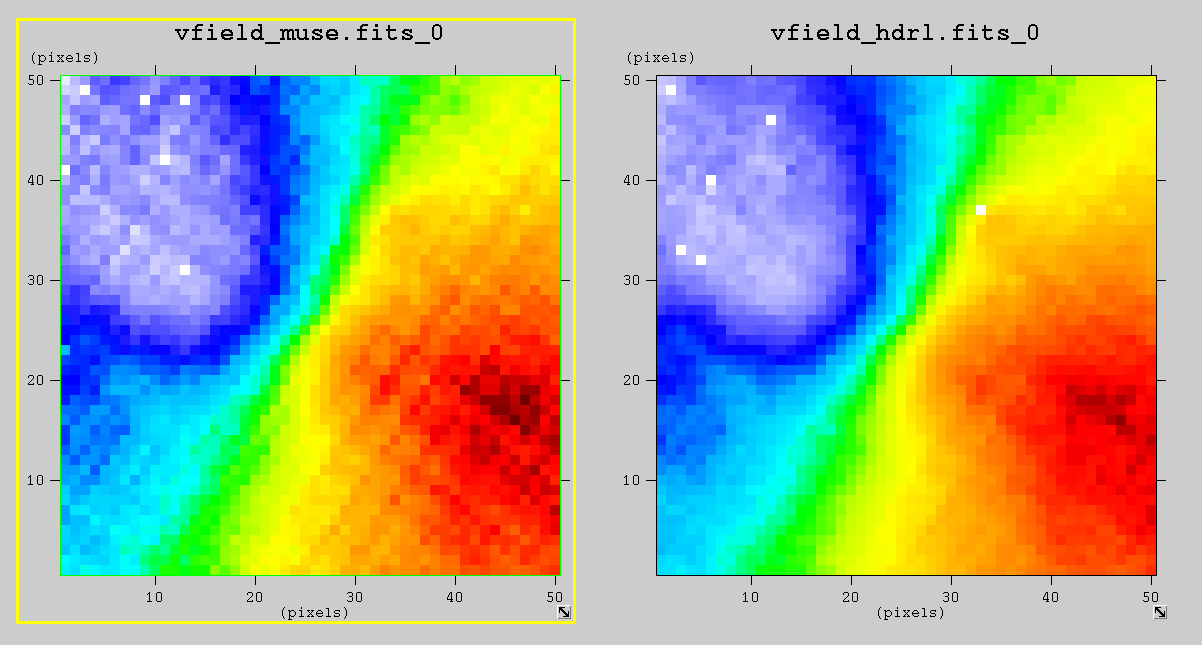
\includegraphics[width=16cm]{figures/FCC184_velocity_field.jpeg}
\caption[] {\footnotesize Comparison between the two-dimensional velocity fields of
  FCC 184 as measured in the MUSE cube (left) and right cube
  (HDRL). The velocity range is from 1220 to 1360 km/sec}
\label{fig:FCC184_velocity_field}
\end{figure}

\begin{figure}[H]
\centering
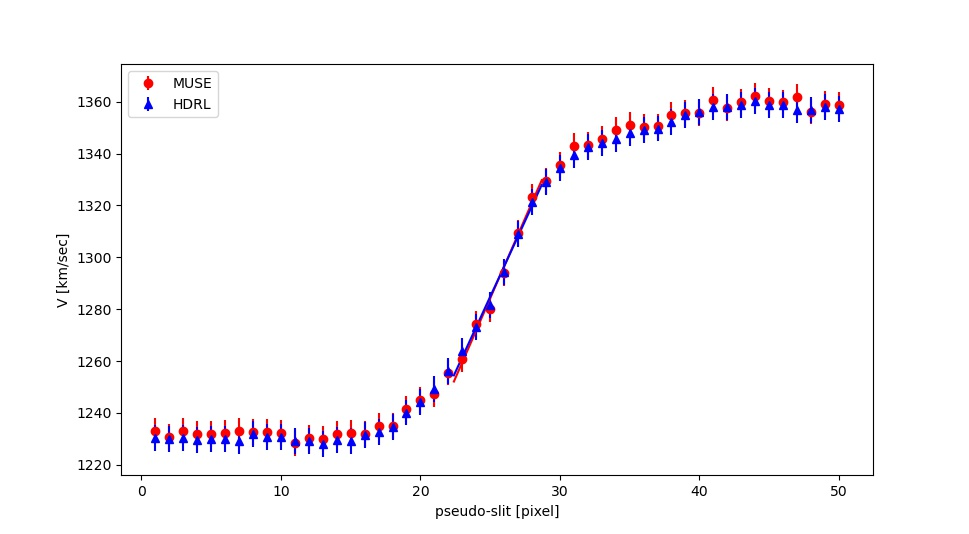
\includegraphics[width=16cm]{figures/FCC184_rotation_velocity.jpeg}
\caption[] {\footnotesize Comparison between the rotation curves extracted from the
  velocity fields (PA $\sim 55^{\circ}$). The central velocity
  gradient is measured from the central 6 pixels (1 pixel = 1.25
  arcsec), and it amounts to $12.3 \pm 0.5$ km/sec/pixel
  ($\sim 9.84 \pm 0.40$ km/sec/arcsec) for the MUSE velocity field and
  $11.7 \pm 0.3$ km/sec/pixel ($9.36 \pm 0.24$ km/sec/arcsec) for the
  HDRL velocity field.}
\label{fig:FCC184_rotation_velocity}
\end{figure}


\subsection{Error Handling in \hdrlresample}
\label{sect:errors}

The routines within \hdrlresample\ allow for the propagation of errors.   To test whether or not the errors are propagated correctly,
a number of synthetic error data sets have been created.   The first set consists of a single and 10 dithered synthetic images with
Gaussian-like errors.   The second set consists of a single and 30 dithered synthetic images with a constant error of 10 e$^-$.

\subsubsection{Gaussian Errors}
The background of each synthetic image was created using the {\tt iraf.mknoise} function with a background level of 500 e$^-$.
with Poisson noise, a gain of 2.5 e$^{-}$/ADU, and a Gaussian readnoise of 5.0 e$^{-}$.   This resulted in synthetic images with a
background of 500 $\pm$ 19.3 e$^-$.   
% std_dev = 55.5
% trim_std_dev = 19.3
% iraf_std = 12.5
A faux error plane was then created by simply taking the square root of the data signal.   This resulted in a synthetic error plane
with an average level of 11.2 $\pm$ 0.3 e$^-$.
% std_dev = 0.59
% trim_std_dev = 0.301
% iraf_std = 0.219

Based on this, we would expect the median error plane of the resampled images with a single synthetic image as input to
be close to the 11.2 $\pm$ 0.3 e$^-$ value.   As can be seen in table \ref{tab:errors}, this is the case for all interpolation methods
except for the {\tt LINEAR} method.  Clearly, the {\tt LINEAR} method is significantly underestimating the error.

For the resampled combination of 10 synthetic images, the error propagation should deliver an average error value of approximately 
$\frac{11.2}{\sqrt{10}}$ = 3.5 e$^-$.  It would appear from table \ref{tab:errors} that the {\tt NEAREST} method significantly over-estimates the error.
However, since the {\tt NEAREST} method takes the nearest value of each pixel in both the area around it, and in the stack of combined frames.
Thus, the {\tt NEAREST} method does not compute a strict average of combined frames, this error value is correct.

%
% For loop-distance=1 ==> 1 pixels goes to 9 pixels.     $\frac{11.2}{\sqrt{10}}/\sqrt{9}$   = 1.18  e$^-$.
% For loop-distance=3 ==> 1 pixels goes to 49 pixels.   $\frac{11.2}{\sqrt{10}}/\sqrt{49}$ = 0.51 e$^-$.
%



\begin{table}
\caption{Error Statistics of the Synthetic Data Images (Normal Errors) and the Resultant Interpolation Images}
\begin{center}
\begin{tabular}{|l|c|c|c|}
\toprule

         Image[ext]$^1$                                       &median              &trim\_mean         &trim\_std\_dev       \\ 
\midrule
         synthetic\_stars\_gal\_bkgd\_1$\ldots$10.fits[2]               &11.199              &11.202              &0.305         \\
\midrule
         hdrldemo\_resample\_DRIZZLE\_single\_1.fits[3]       &11.165              &11.151              &0.464         \\
         hdrldemo\_resample\_DRIZZLE\_single\_3.fits[3]       &11.165              &11.151              &0.464         \\
         hdrldemo\_resample\_LANCZOS\_single\_1.fits[3]       &11.134              &11.121              &3.278         \\
         hdrldemo\_resample\_LANCZOS\_single\_3.fits[3]       &11.146              &11.135              &3.180         \\
         hdrldemo\_resample\_LINEAR\_single\_1.fits[3]        &8.969  			&8.958  &0.395         \\
         hdrldemo\_resample\_LINEAR\_single\_3.fits[3]        &6.381  			&6.374  &0.401         \\
         hdrldemo\_resample\_NEAREST\_single\_1.fits[3]       &11.165              &11.151              &0.464         \\
         hdrldemo\_resample\_NEAREST\_single\_3.fits[3]       &11.165              &11.151              &0.464         \\
         hdrldemo\_resample\_QUADRATIC\_single\_1.fits[3]     &11.076              &11.062              &0.514         \\
         hdrldemo\_resample\_QUADRATIC\_single\_3.fits[3]     &11.000              &10.986              &0.818         \\
         hdrldemo\_resample\_RENKA\_single\_1.fits[3]         &11.143              &11.129              &0.488         \\
         hdrldemo\_resample\_RENKA\_single\_3.fits[3]         &11.144              &11.131              &0.487         \\
\midrule 
         hdrldemo\_resample\_DRIZZLE\_coadd\_1.fits[3]        &2.503		   &2.544               &0.900         \\
         hdrldemo\_resample\_DRIZZLE\_coadd\_3.fits[3]        &2.503               &2.544               &0.900         \\
         hdrldemo\_resample\_LANCZOS\_coadd\_1.fits[3]        &2.653               &2.699               &0.961         \\
         hdrldemo\_resample\_LANCZOS\_coadd\_3.fits[3]        &2.926               &2.983               &1.110         \\
         hdrldemo\_resample\_LINEAR\_coadd\_1.fits[3]         &1.323               &1.346               &0.502         \\
         hdrldemo\_resample\_LINEAR\_coadd\_3.fits[3]         &0.632               &0.645               &0.240         \\
         hdrldemo\_resample\_NEAREST\_coadd\_1.fits[3]        &11.162 	   &11.148 		&0.450         \\
         hdrldemo\_resample\_NEAREST\_coadd\_3.fits[3]        &11.162          &11.148 			&0.450         \\
         hdrldemo\_resample\_QUADRATIC\_coadd\_1.fits[3]      &1.703               &1.733               &0.624         \\
         hdrldemo\_resample\_QUADRATIC\_coadd\_3.fits[3]      &1.199               &1.222               &0.430         \\
         hdrldemo\_resample\_RENKA\_coadd\_1.fits[3]          &2.149               &2.186               &0.778         \\
         hdrldemo\_resample\_RENKA\_coadd\_3.fits[3]          &2.126               &2.165               &0.776         \\
\bottomrule

\end{tabular}	
\end{center}																											

\label{tab:errors}
\noindent{
		$^1$ The image and the [extension] of the error frame. \\
		}
\end{table}



\subsubsection{Constant Errors}

For this data set,  a faux error plane was then created and set to a constant value of 10 e$^-$. 
Based on this, we would expect the error plane of the resampled images with a single synthetic image as input to
be close to the 10.0 $\pm$ 0.0 e$^-$ value.   As can be seen in table \ref{tab:errors_fixed}, this is the case for all interpolation methods
except for the {\tt LINEAR} method.  Clearly, the {\tt LINEAR} method is again underestimating the error when a single image is being resampled.

For the resampled combination of 30 synthetic images, the error propagation should deliver an average error value of approximately 
$\frac{10.0}{\sqrt{30}}$ = 1.83 e$^-$.  As can be seen in table \ref{tab:errors_fixed}, the {\tt LINEAR} method slightly under-estimates the error.
The same may be true of the {\tt QUADRATIC} method.
It would also appear that the {\tt NEAREST} method significantly over-estimates the error.
However, since the {\tt NEAREST} method takes the nearest value of each pixel in both the area around it, and in the stack of combined frames, this
value is correct.  



\begin{table}[H]
\caption{Error Statistics of the Synthetic Data Images (Fixed Errors) and the Resultant Interpolation Images}
\begin{center}
\begin{tabular}{|l|c|c|c|}
\toprule

         Image[ext]$^1$                                       				&median              &trim\_mean         &trim\_std\_dev       \\ 
\midrule
         synthetic\_stars\_gal\_bkgd\_1$\ldots$30.fits[2]               &10.00              &10.00              &0.00         \\
\midrule
hdrldemo\_resample\_DRIZZLE\_single\_1.fits[3]             & 10.000      & 10.000     & 0.000         \\
hdrldemo\_resample\_DRIZZLE\_single\_3.fits[3]             & 10.000      & 10.000     & 0.000         \\
hdrldemo\_resample\_LANCZOS\_single\_1.fits[3]             & 9.971       & 9.971     & 2.869         \\
hdrldemo\_resample\_LANCZOS\_single\_3.fits[3]             & 9.979       & 9.979      & 2.795         \\
hdrldemo\_resample\_LINEAR\_single\_1.fits[3]              & 8.031      & 8.031      & 0.122         \\
hdrldemo\_resample\_LINEAR\_single\_3.fits[3]              & 5.713       & 5.713      & 0.271         \\
hdrldemo\_resample\_NEAREST\_single\_1.fits[3]             & 10.000      & 10.000     & 0.000         \\
hdrldemo\_resample\_NEAREST\_single\_3.fits[3]             & 10.000      & 10.000     & 0.000         \\
hdrldemo\_resample\_QUADRATIC\_single\_1.fits[3]           & 9.920       & 9.920      & 0.205         \\
hdrldemo\_resample\_QUADRATIC\_single\_3.fits[3]           & 9.852       & 9.852      & 0.605         \\
hdrldemo\_resample\_RENKA\_single\_1.fits[3]               & 9.981       & 9.981      & 0.141         \\
hdrldemo\_resample\_RENKA\_single\_3.fits[3]               & 9.980       & 9.980      & 0.143         \\
\midrule
hdrldemo\_resample\_DRIZZLE\_coadd\_1.fits[3]              & 1.291       & 1.320      & 0.533         \\
hdrldemo\_resample\_DRIZZLE\_coadd\_3.fits[3]              & 1.291       & 1.320      & 0.533         \\
hdrldemo\_resample\_LANCZOS\_coadd\_1.fits[3]              & 1.368       & 1.399      & 0.564         \\
hdrldemo\_resample\_LANCZOS\_coadd\_3.fits[3]              & 1.509       & 1.547      & 0.619         \\
hdrldemo\_resample\_LINEAR\_coadd\_1.fits[3]               & 0.683       & 0.698      & 0.281         \\
hdrldemo\_resample\_LINEAR\_coadd\_3.fits[3]               & 0.326       &0.334      & 0.137         \\
hdrldemo\_resample\_NEAREST\_coadd\_1.fits[3]              & 10.000      & 10.000     & 0.000         \\
hdrldemo\_resample\_NEAREST\_coadd\_3.fits[3]              & 10.000      & 10.000     & 0.000         \\
hdrldemo\_resample\_QUADRATIC\_coadd\_1.fits[3]            & 0.878       & 0.898      & 0.363         \\
hdrldemo\_resample\_QUADRATIC\_coadd\_3.fits[3]            & 0.618       & 0.634     & 0.252         \\
hdrldemo\_resample\_RENKA\_coadd\_1.fits[3]                & 1.108       & 1.133      & 0.457         \\
hdrldemo\_resample\_RENKA\_coadd\_3.fits[3]                & 1.096       & 1.122      & 0.452         \\
\bottomrule

\end{tabular}	
\end{center}																											

\label{tab:errors_fixed}
\noindent{
		$^1$ The image and the [extension] of the error frame. \\
		}
\end{table}



